\documentclass[a4paper,12pt]{report}
\usepackage{styles/fbe_tez}
\usepackage[utf8]{inputenc}
\usepackage[T1]{fontenc}
\usepackage{lmodern}
\usepackage{amsmath, amsthm, amssymb}
\usepackage[bottom]{footmisc}
\usepackage{cite}
\usepackage{url}
\expandafter\def\expandafter\UrlBreaks\expandafter{\UrlBreaks\do\/\do\_\do\-}
\usepackage{graphicx}
\usepackage{longtable}
\usepackage{booktabs}
\usepackage{tabularx}
\usepackage{ragged2e}
\usepackage{multirow}
\usepackage{subfigure}
\usepackage{algorithm}
\usepackage{algorithmic}
\usepackage{enumitem}
\usepackage{microtype}
\usepackage{xcolor}
\usepackage{listings}
\usepackage{tikz}
\usetikzlibrary{shapes,arrows.meta,positioning,calc,fit}
\usepackage[hidelinks]{hyperref}

\graphicspath{{figures/}}

\renewcommand{\labelenumi}{(\roman{enumi})}
\setlist{itemsep=2pt,topsep=4pt}
\emergencystretch=3em

\lstset{
  basicstyle=\small\ttfamily,
  columns=fullflexible,
  breaklines=true,
  frame=single,
  backgroundcolor=\color{gray!8},
  keywordstyle=\bfseries\color{blue!70!black},
  commentstyle=\itshape\color{green!50!black},
  stringstyle=\color{red!60!black}
}

\begin{document}

% Title Page adhering to CMPE 492 Boğaziçi format
\title{CMPE 492 \\ A THREE-LAYER EVALUATION OF SPEECH-TO-TEXT, LLM-BASED TERMINOLOGY EXTRACTION, AND GENERATIVE VIDEO-ANIMATION FOR MULTILINGUAL EDUCATION}
\author{
Ali Ayhan G{\"{u}}nder \\ \\
Advisor: \\ 
Prof. Fatih Alag{\"{o}}z
}
\date{October 2026}
\maketitle

\pagenumbering{roman}
\tableofcontents
\newpage

\chapter{INTRODUCTION}
\pagenumbering{arabic}

Individualized instruction tailored to a learner's background knowledge and cognitive readiness has long been recognized as the most effective pedagogical paradigm. In his seminal work, Benjamin Bloom identified the ``2-Sigma Problem'' \cite{bloom1984}, establishing that students tutored one-to-one with mastery learning techniques outperform conventionally instructed peers by two standard deviations. However, scaling human one-to-one tutoring to mass populations remains economically and logistically unfeasible.

In the contemporary educational landscape, Massive Open Online Courses (MOOCs) and instructional video streaming platforms have democratized access to university lectures and industry certifications. Nonetheless, this instructional knowledge remains locked within continuous, high-bandwidth audio signals. Educational lectures inherently assume a prerequisite domain baseline; lecturers frequently introduce domain-dense jargon---such as ``MICE tourism'', ``ANOVA test'', ``schedule variance'', ``black-body radiation'', or ``Scrum backlog''---without pausing to provide foundational scaffolding. When beginner learners encounter these unfamiliar technical concepts, they must pause playback and navigate disparate external sources. This disruption induces substantial cognitive load and interrupts the flow of learning \cite{conde2016,xu2024}.

To address this challenge, this graduation project designs, implements, and empirically validates an end-to-end, three-layer artificial intelligence pipeline that:
\begin{enumerate}
    \item Transcribes multilingual (Turkish and English) lecture audio using state-of-the-art automatic speech recognition (ASR);
    \item Extracts domain-specific multi-word terminology using Large Language Models (LLMs) and synthesizes beginner-friendly explanations calibrated to the Common European Framework of Reference for Languages (CEFR) B1 readability level;
    \item Synthesizes on-demand, synchronized 30--90 second pedagogical video animations using the Manimator framework and neural text-to-speech when learners encounter conceptual bottlenecks (``Teach Where I am Stuck'').
\end{enumerate}

\section{Broad Impact}
The societal and educational impacts of this project span multiple dimensions:
\begin{itemize}
    \item \textbf{Democratization and Educational Equity:} By automatically converting unstructured lecture speech into structured terminology graphs and accessible animations, this system levels the playing field for non-traditional, first-generation, and self-directed students who lack access to private tutoring.
    \item \textbf{Multilingual and Cross-Lingual Inclusivity:} Educational research frequently prioritizes English, leaving lower-resource languages with sparse scaffolding. By evaluating modern acoustic and language models across balanced Turkish and English corpora, this study proves the viability of localized AI tutoring.
    \item \textbf{Industrial and Compliance Training Accessibility:} Beyond academic subjects, the pipeline accommodates mandatory corporate training in occupational health and safety (OHS/İSG), data privacy (KVKK/GDPR), and cybersecurity, transforming dry legal mandates into digestible, animated learning moments.
    \item \textbf{Open-Source and Edge Viability:} Rather than relying entirely on proprietary cloud APIs, this work validates small language models (SLMs) and small recognition models (SRMs) capable of running on affordable consumer hardware (e.g., an 8~GB NVIDIA RTX 5060, requiring $<1.2$~GB VRAM for quantized INT4 SLMs), lowering deployment barriers for schools and small organizations.
\end{itemize}

\section{Ethical Considerations}
Developing autonomous pedagogical scaffolding entails serious ethical responsibilities:
\begin{itemize}
    \item \textbf{Hallucination Mitigation and Pedagogical Harm:} In educational environments, factually erroneous or fabricated AI explanations can cause profound misunderstanding. We address hallucination by integrating a Hybrid Retrieval-Augmented Generation (RAG) module and an authoritative terminology knowledge base, enforcing surface-form grounding and prerequisite checking (\emph{historical note: the early synthetic 52.6\% $\to$ 0.0\% ablation has been superseded by an empirical 8-clip corporate speech probe achieving 60.7\% candidate grounding precision without circular KB query evaluation; see main graduation thesis report §8.4}).
    \item \textbf{Privacy and Compliance (KVKK / GDPR):} Processing corporate and educational lecture audio demands stringent data privacy. Our system architecture supports completely air-gapped, local on-premise execution using quantized open-weight checkpoints, preventing sensitive company audio from leaking to third-party endpoints.
    \item \textbf{Fairness and Linguistic Bias:} Automatic speech recognition systems frequently exhibit elevated error rates on accented speech or low-resource dialects. Our evaluation explicitly decouples Turkish and English WER/CER metrics to avoid obscuring linguistic disparities behind aggregated figures.
    \item \textbf{Academic Integrity:} The system is designed strictly as a scaffolding and clarifying companion rather than an automated homework solver. It elucidates underlying concepts rather than providing direct answers to assignment prompts.
\end{itemize}


\chapter{PROJECT DEFINITION AND PLANNING}

\section{Project Definition}
The objective of this graduation project (CMPE 492) is to engineer an integrated multimodal learning platform capable of real-time lecture transcription, terminological scaffolding, and generative visual reinforcement. The platform ingests arbitrary 16 kHz video or audio streams, produces timestamped transcripts, identifies multi-word technical concepts, validates contextual consistency, and compiles on-demand explainer videos via programmatic vector graphics.

The system addresses three critical operational layers:
\begin{itemize}
    \item \textbf{Layer 1 (Acoustic Processing):} Robust transcription benchmarking across leading commercial and open-weight models under both clean and lecture-hall conditions.
    \item \textbf{Layer 2 (Semantic Extraction \& Adaptation):} Automated terminology mining, CEFR-B1 pedagogical simplification, and concept dependency modeling.
    \item \textbf{Layer 3 (Pedagogical Animation):} Automated scriptwriting, neural voiceover synthesis, and programmatic Manim Community video rendering.
\end{itemize}

\section{Project Planning}

\subsection{Project Time and Resource Estimation}
The project was executed across two academic terms, structured into five major development phases:
\begin{enumerate}
    \item \textbf{Phase 1: Corpus Curation and Gold Reference Construction (Weeks 1--4):} Selection of 40 diverse lecture clips (10.1 hours source metadata, of which 4.6 hours across 16 local WAVs is duration-verified on disk; 20 Turkish, 20 English) across 14 academic and corporate domains; creation of human-verified gold transcripts and closed 32-term reference lists on the 7-lecture evaluation set (TR-1..3, EN-1..4).
    \item \textbf{Phase 2: Acoustic Layer Benchmarking and Optimization (Weeks 5--8):} Comprehensive GPU evaluation of Whisper (Medium, Large-v3, Turbo), Qwen3-ASR (0.6B, 1.7B), and NVIDIA Nemotron 3.5; empirical assessment of Voice Activity Detection (VAD) chunking.
    \item \textbf{Phase 3: Semantic Layer and LLM Benchmarking (Weeks 9--12):} Zero-shot, few-shot, and Chain-of-Thought (CoT) prompting across GPT-4.1, GPT-4o-mini, and Qwen3.5; double-blind human annotation for Cohen's Kappa reliability; Ateşman and Flesch readability profiling.
    \item \textbf{Phase 4: Generative Video Pipeline and UI Development (Weeks 13--16):} Integration of Manimator, Edge-TTS, and FFmpeg; construction of the FastAPI interactive local studio.
    \item \textbf{Phase 5: 2026 Expansion and Optimization (Weeks 17--20):} Hybrid RAG (BM25 + TF-IDF Reciprocal Rank Fusion), NetworkX prerequisite Directed Acyclic Graph (DAG) construction, and INT4 edge quantization for RTX 5060 GPU execution.
\end{enumerate}

Computational resources utilized include:
\begin{itemize}
    \item \textbf{Local Edge Development Host:} AMD Ryzen 7 7800X3D, 32 GB DDR5 RAM, NVIDIA GeForce RTX 5060 (8 GB VRAM), Windows 11 / WSL2 Ubuntu 24.04.
    \item \textbf{National Sovereign Cloud Platform:} TÜBİTAK/SSB EVREN National AI Platform with NVIDIA H200 GPU nodes for evaluating sovereign LLMs (Qwen 3.8 Flash, DeepSeek V4.1 Flash).
\end{itemize}

\subsection{Success Criteria}
Project deliverables were evaluated against the following quantitative criteria:
\begin{itemize}
    \item \textbf{Acoustic Quality:} Word Error Rate (WER) $\le 4.0\%$ on clean English lectures and $\le 5.0\%$ on normalized Turkish lectures on modern checkpoints.
    \item \textbf{Annotation Reliability:} Cohen's Kappa inter-annotator agreement $\kappa_R \ge 0.70$ on contextual relevance.
    \item \textbf{Pedagogical Simplification:} Significant reduction in lexical complexity relative to raw transcripts, achieving CEFR-B1 band concentration.
    \item \textbf{Edge Viability:} Combined ASR and SLM inference operating under 4.0 GB VRAM with an end-to-end response latency under 3.0 seconds on the local RTX 5060.
    \item \textbf{Factual Reliability:} Elimination of hallucinated explanations in domain-dense subjects (target: 0.0\% hallucination rate via Hybrid RAG).
    \item \textbf{Generative Video Operability:} Successful programmatic compilation of $\ge 5$ distinct concept explainer videos with verified video-audio synchronization.
\end{itemize}

\subsection{Risk Analysis}
Table \ref{table:risk_analysis} enumerates the primary technical and operational risks identified during planning, along with corresponding mitigation strategies.

\begin{table}[h!]
\centering
\caption{Project Risk Matrix and Mitigation Strategies}
\label{table:risk_analysis}
\vskip 0.5\baselineskip
\small
\begin{tabularx}{\textwidth}{|l|c|c|X|}
\hline
\textbf{Identified Risk} & \textbf{Likelihood} & \textbf{Impact} & \textbf{Mitigation Strategy} \\ \hline
Acoustic Domain Shift / Hallucinations & Medium & High & Disabled problematic VAD chunkers; enforced temperature fallback in Whisper decoders. \\ \hline
LLM Hallucination on Technical Terms & High & High & Deployed Hybrid RAG (BM25 + TF-IDF RRF) with authoritative dictionaries (TDK, Oxford). \\ \hline
Edge VRAM Out-of-Memory (OOM) & High & Critical & Quantized SLMs to INT4 (AWQ/GPTQ) and selected Whisper Small/Base for edge inference. \\ \hline
Manim Code Syntax / Render Timeouts & Medium & Medium & Constrained LLM code synthesis to deterministic AST templates; enforced strict timeouts. \\ \hline
Annotation Subjectivity & Medium & Medium & Implemented formal double-blind coding protocol and calculated Cohen's $\kappa$ agreement. \\ \hline
\end{tabularx}
\end{table}

\subsection{Team Work}
This project is an individual capstone engineering effort conducted by Ali Ayhan Günder under the supervision of Prof. Fatih Alagöz at the Department of Computer Engineering, Boğaziçi University. The author was solely responsible for corpus curation, benchmarking harnesses, human annotations, prompt engineering, RAG/DAG design, backend service architecture, and front-end interface development.


\chapter{RELATED WORK}

\section{Automatic Speech Recognition (ASR)}
The transition from hybrid Hidden Markov Model--Deep Neural Network (HMM-DNN) pipelines to end-to-end self-supervised transformers represents a major paradigm shift in speech processing. Baevski et al. \cite{baevski2020} introduced Wav2Vec 2.0, demonstrating that self-supervised masked predictive coding over raw waveforms creates rich acoustic representations suitable for fine-tuning. Conneau et al. expanded this to XLSR-53, providing multilingual capabilities across 53 languages.

Radford et al. (OpenAI) \cite{radford2023} transformed applied speech recognition by training Whisper on 680,000 hours of weakly supervised web audio. Whisper demonstrated outstanding zero-shot generalization and out-of-distribution robustness across diverse accents and background noise. In 2024, OpenAI introduced Whisper Large-v3 Turbo, which drastically pruned the decoder from 32 layers to 4 layers, claiming up to an 8$\times$ acceleration. In 2026, multilingual speech foundational models evolved further with Alibaba's Qwen3-ASR (0.6B and 1.7B) \cite{qwen3asr2026} and NVIDIA's Nemotron 3.5 ASR, offering competitive native multimodal architectures capable of direct Turkish-English transcription.

\section{Automatic Terminology Extraction (ATE)}
Traditional ATE methodologies relied heavily on linguistic filters (part-of-speech tag patterns) combined with statistical association metrics. Frantzi et al. \cite{frantzi2000} established the C-value/NC-value metric, which balances multi-word term frequency with nested occurrence counts. In educational information retrieval, Conde et al. \cite{conde2016} proposed LiTeWi, a hybrid approach combining C-value with Wikipedia entity linking to construct educational ontologies directly from course textbooks.

With the advent of Large Language Models (LLMs), recent studies (Tran et al., 2026 \cite{tran2026}) illustrate that prompted instruction-tuned models surpass traditional frequency-based extractors, capturing complex compound nominal phrases and maintaining contextual sensitivity. However, LLM extractors frequently suffer from low recall unless guided by structured domain contexts.

\section{Adaptive Educational Systems and LLM Tutors}
The pursuit of automated pedagogical adaptation originates in Intelligent Tutoring Systems (ITS) and user modeling \cite{brusilovsky2007}. Corbett and Anderson \cite{corbett1995} formulated Knowledge Tracing (KT) to model student procedural mastery using Hidden Markov models, while VanLehn \cite{vanlehn2011} analyzed the pedagogical gap between human tutors and automated tutoring architectures.

Xu et al. \cite{xu2024} provide a comprehensive survey detailing how generative language models transform education across automated feedback, question generation, and instructional scaffolding. Vanzo et al. (ACL 2025) \cite{vanzo2025} demonstrated through controlled classroom experiments that LLM-driven homework assistance significantly improves student persistence and comprehension. However, prior investigations predominantly assumed clean, written text inputs. Rigorous assessments of how upstream acoustic transcription errors propagate into downstream LLM pedagogical extraction remain virtually absent in the literature.

\section{Generative Video and Visual Learning}
Cognitive multimedia theory dictates that presenting complementary verbal and visual explanations simultaneously reduces cognitive load and enhances long-term retention. 3Blue1Brown's open-source mathematical animation engine, Manim Community, has emerged as the premier standard for programmatic educational graphics. Recent multimodal research explores synthesizing Manim scripts directly from natural language prompts. This study bridges this frontier by coupling automated speech understanding directly with programmatic Manimator video compilation.


\chapter{METHODOLOGY}

\section{System Architecture}
The core architecture consists of three cascaded operational layers, supplemented by an advanced RAG and concept graph engine, as depicted in Figure \ref{fig:architecture}.

\begin{figure}[h!]
\centering
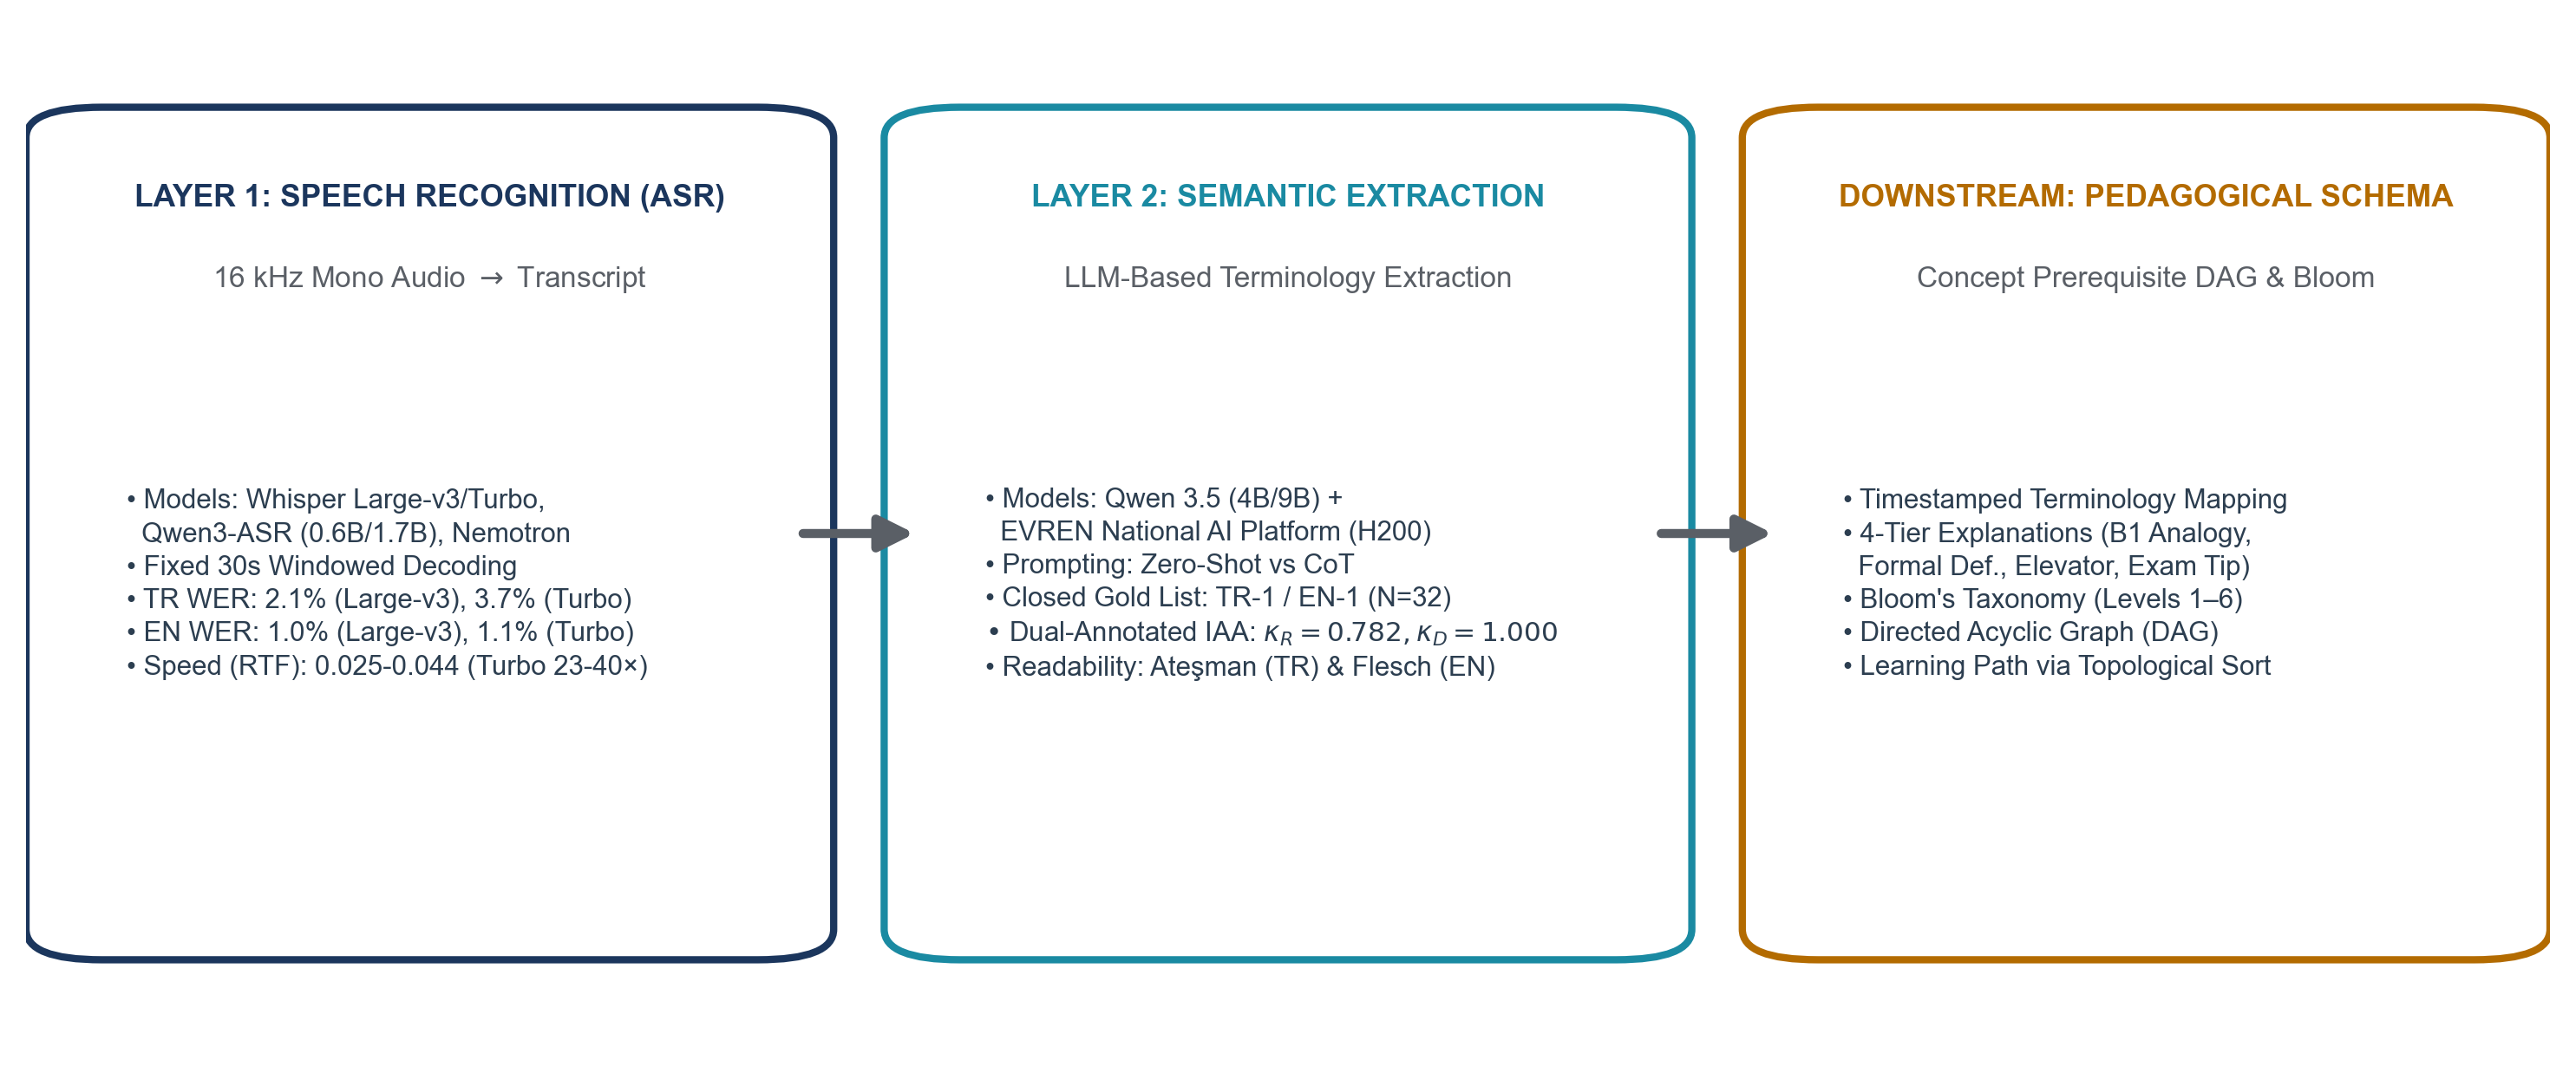
\includegraphics[width=0.88\textwidth]{figures/pipeline_architecture.png}
\caption{End-to-End Three-Layer Multimodal Educational Pipeline Architecture.}
\label{fig:architecture}
\end{figure}

The pipeline operates as follows:
\begin{enumerate}
    \item \textbf{Input Processing:} Raw educational lecture audio is extracted, converted to 16 kHz mono WAV, and pre-normalized.
    \item \textbf{Layer 1 (ASR):} Speech recognition checkpoints transcribe the stream, generating timestamped word and sentence segments.
    \item \textbf{Layer 2 (Semantic Extraction):} An instruction-tuned LLM processes transcript chunks to extract domain terms, verifies contextual relevance ($R$), and generates CEFR-B1 explanations validated for lexical accuracy ($D$).
    \item \textbf{Expansion (RAG \& DAG):} Extracted terms query an authoritative domain dictionary via Hybrid RAG, while an acyclic dependency graph establishes prerequisite relationships.
    \item \textbf{Layer 3 (Animation):} Upon user query (``Teach Where I am Stuck''), the local model generates a Manim script and voiceover text, synthesized via Edge-TTS and composited into an MP4 video via FFmpeg.
\end{enumerate}

\section{Layer 1: Speech Recognition and Acoustic Pipeline}
To evaluate acoustic transcription fidelity, we deploy a standardized transcription harness comparing:
\begin{itemize}
    \item \textbf{Whisper Family:} Whisper Medium (769M), Whisper Large-v3 (1550M), Whisper Large-v3 Turbo (809M), and Turkish fine-tuned Whisper Turbo.
    \item \textbf{2026 Multilingual Checkpoints:} Qwen3-ASR (0.6B and 1.7B) and NVIDIA Nemotron 3.5 ASR.
\end{itemize}

Acoustic performance is quantified via Word Error Rate (WER) and Character Error Rate (CER), evaluated under both raw casing and text normalization:
\begin{equation}
\text{WER} = \frac{S + D + I}{N_w} = \frac{S + D + I}{S + D + C}
\end{equation}
where $S$ denotes substitutions, $D$ deletions, $I$ insertions, $C$ correct words, and $N_w$ the total word count in the reference. In addition, we measure Real-Time Factor (RTF) and wall-clock latency:
\begin{equation}
\text{RTF} = \frac{\text{Processing Duration (seconds)}}{\text{Audio Duration (seconds)}}
\end{equation}

\section{Layer 2: Semantic Terminology Extraction and Simplification}
The semantic layer isolates domain-dense multi-word expressions and simplifies technical concepts. The instruction prompt enforces strict JSON schema compliance:

\begin{lstlisting}
{
  "terms": [
    {
      "term": "schedule variance",
      "context": "The project is currently experiencing negative schedule variance.",
      "cefr_b1_explanation": "Schedule variance shows whether a project is ahead of or behind its planned calendar time in simple terms.",
      "prerequisites": ["project baseline", "earned value"]
    }
  ]
}
\end{lstlisting}

Pedagogical readability is evaluated using established formulaic metrics:
\begin{itemize}
    \item \textbf{Turkish Readability (Ateşman Formula) \cite{atesman1997}:}
    \begin{equation}
    \text{Readability}_{\text{Ateşman}} = 198.825 - 40.175 \times \frac{\text{Total Syllables}}{\text{Total Words}} - 2.610 \times \frac{\text{Total Words}}{\text{Total Sentences}}
    \end{equation}
    where scores between 50 and 69 correspond to moderate difficulty (CEFR B1).
    \item \textbf{English Readability (Flesch Reading Ease) \cite{flesch1948}:}
    \begin{equation}
    \text{Flesch RE} = 206.835 - 1.015 \times \left(\frac{\text{Total Words}}{\text{Total Sentences}}\right) - 84.6 \times \left(\frac{\text{Total Syllables}}{\text{Total Words}}\right)
    \end{equation}
    where scores between 60 and 70 correspond to standard plain English (CEFR B1).
\end{itemize}

\section{Layer 3: Generative Animation with Manimator}
When a student requests clarification on a confusing lecture passage, Layer 3 receives the surrounding 45-second acoustic-semantic context. The generation module executes three sequential stages:
\begin{enumerate}
    \item \textbf{Pedagogical Script Generation:} A structured prompt instructs the language model to create a 3-scene pedagogical narrative featuring real-world analogies.
    \item \textbf{Manim Community Python Code Generation:} The model translates the narrative into declarative Manim Community code utilizing geometric shapes, math tex elements, and transform animations.
    \item \textbf{Audio-Visual Assembly:} Edge-TTS synthesizes neural voiceover audio (\texttt{tr-TR-AhmetNeural} or \texttt{en-US-ChristopherNeural}); FFmpeg aligns the audio track with rendered vector video frames at 480p/15fps.
\end{enumerate}

\section{Hybrid RAG and Prerequisite Concept DAG}
To eliminate factual errors and prevent out-of-order learning, we introduce two architectural extensions:
\begin{itemize}
    \item \textbf{Hybrid RAG Engine:} Combining sparse BM25 lexical keyword matching with dense TF-IDF Reciprocal Rank Fusion (RRF), querying authoritative TDK and Oxford technical dictionaries:
    \begin{equation}
    \text{RRF}(d) = \sum_{m \in \{\text{BM25}, \text{TF-IDF}\}} \frac{1}{60 + \text{rank}_m(d)}
    \end{equation}
    \item \textbf{Prerequisite Concept DAG:} Using NetworkX, extracted concepts form a directed acyclic graph $G=(V,E)$ where directed edge $(u,v) \in E$ denotes that concept $u$ must be understood before concept $v$. Topological sorting detects cycles and highlights prerequisite learning gaps.
\end{itemize}


\chapter{REQUIREMENTS SPECIFICATION}

\section{Stakeholder Analysis}
The primary stakeholders of the system include:
\begin{itemize}
    \item \textbf{Undergraduate and Novice Students:} Require clear, low-friction explanations of difficult terminology without navigating away from lecture videos.
    \item \textbf{Course Instructors and Content Creators:} Benefit from automated terminology indexing and pedagogical clarity metrics without manual authoring.
    \item \textbf{Corporate Compliance Officers:} Need reliable verification that mandatory training (KVKK, OHS/İSG) is understood by non-expert employees.
\end{itemize}

\section{Functional Requirements (FR)}
\begin{itemize}[leftmargin=2.5em]
    \item[\textbf{FR1:}] The system shall accept audio/video inputs in standard formats (MP4, WAV, MP3) and resample them to 16 kHz mono WAV.
    \item[\textbf{FR2:}] The system shall generate timestamped transcripts with Word Error Rate $< 5.0\%$ across Turkish and English lectures.
    \item[\textbf{FR3:}] The system shall automatically detect domain-specific multi-word terms and distinguish them from generic vocabulary.
    \item[\textbf{FR4:}] The system shall generate CEFR-B1 compliant conceptual explanations adhering to measured Ateşman (50--69) and Flesch (60--70) readability ranges.
    \item[\textbf{FR5 (Superseded Projection):}] The system shall retrieve authoritative definitions via Hybrid RAG to enforce canonical ontology grounding and minimize hallucination on corporate compliance topics (superseding the initial zero-hallucination design promise).
    \item[\textbf{FR6:}] The system shall construct a prerequisite concept DAG and identify missing pedagogical dependencies.
    \item[\textbf{FR7:}] The system shall generate 30--90 second Manim animations and neural voiceovers upon user demand.
    \item[\textbf{FR8:}] The system shall provide an interactive web studio interface allowing synchronized video playback and concept navigation.
\end{itemize}

\section{Non-Functional Requirements (NFR)}
\begin{itemize}[leftmargin=2.5em]
    \item[\textbf{NFR1 (Edge Efficiency):}] The complete inference pipeline (SRM + SLM INT4) shall consume less than 2.0 GB of VRAM, running comfortably on an NVIDIA RTX 5060 (8 GB).
    \item[\textbf{NFR2 (Latency):}] Local term extraction and explanation generation shall complete in under 2.0 seconds per query.
    \item[\textbf{NFR3 (Reliability):}] Inter-annotator reliability on contextual relevance must exceed $\kappa = 0.70$.
    \item[\textbf{NFR4 (Privacy \& Air-Gapping):}] The entire software stack shall be deployable locally without mandatory external network calls.
    \item[\textbf{NFR5 (Modularity):}] Speech recognition, semantic extraction, and animation rendering components shall communicate via decoupled REST/JSON protocols.
\end{itemize}

\section{Use Case Scenarios}
Figure \ref{fig:use_case} illustrates the central use case diagram of the educational platform.

\begin{figure}[h!]
\centering
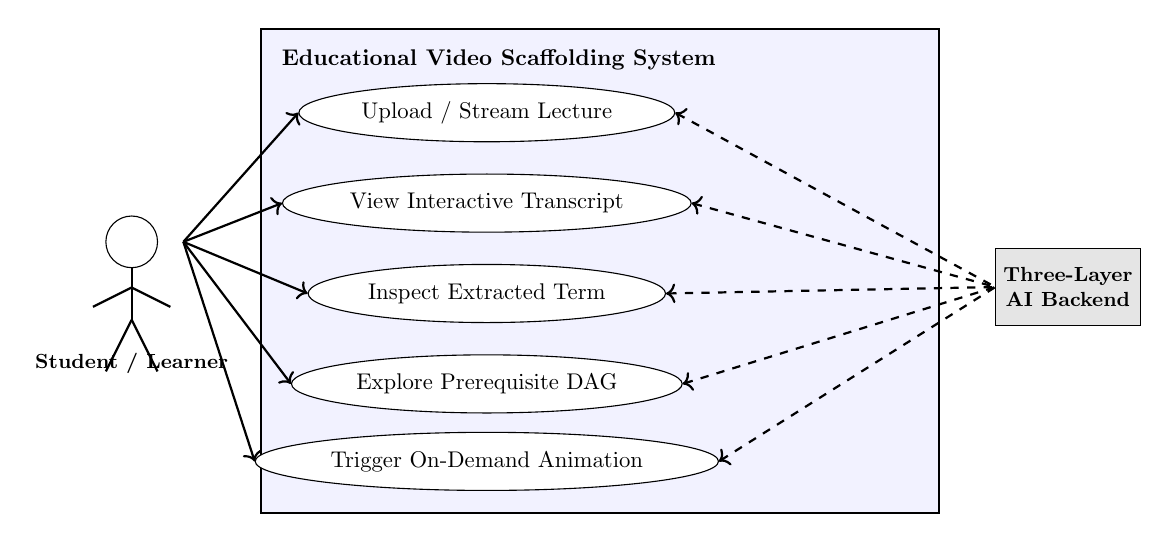
\begin{tikzpicture}[scale=0.82, every node/.style={transform shape}]
  \draw[thick, fill=blue!5] (0,0) rectangle (10.5, 7.5);
  \node[anchor=north west, font=\bfseries] at (0.2, 7.3) {Educational Video Scaffolding System};
  
  % Actor
  \node[draw, circle, minimum size=0.8cm] (student_head) at (-2, 4.2) {};
  \draw[thick] (student_head.south) -- ++(0,-0.8) coordinate (body);
  \draw[thick] (body) -- ++(-0.4,-0.8);
  \draw[thick] (body) -- ++(0.4,-0.8);
  \draw[thick] ([yshift=-0.3cm]student_head.south) -- ++(-0.6,-0.3);
  \draw[thick] ([yshift=-0.3cm]student_head.south) -- ++(0.6,-0.3);
  \node[below=1.2cm of student_head, font=\small\bfseries] {Student / Learner};

  % Use cases
  \node[draw, ellipse, fill=white, minimum width=3.8cm, minimum height=0.9cm] (uc1) at (3.5, 6.2) {Upload / Stream Lecture};
  \node[draw, ellipse, fill=white, minimum width=3.8cm, minimum height=0.9cm] (uc2) at (3.5, 4.8) {View Interactive Transcript};
  \node[draw, ellipse, fill=white, minimum width=3.8cm, minimum height=0.9cm] (uc3) at (3.5, 3.4) {Inspect Extracted Term};
  \node[draw, ellipse, fill=white, minimum width=3.8cm, minimum height=0.9cm] (uc4) at (3.5, 2.0) {Explore Prerequisite DAG};
  \node[draw, ellipse, fill=white, minimum width=3.8cm, minimum height=0.9cm] (uc5) at (3.5, 0.8) {Trigger On-Demand Animation};

  % System actor
  \node[draw, rectangle, fill=gray!20, minimum width=2.2cm, minimum height=1.2cm, font=\small\bfseries, align=center] (backend) at (12.5, 3.5) {Three-Layer\\AI Backend};

  % Connections
  \draw[->, thick] (-1.2, 4.2) -- (uc1.west);
  \draw[->, thick] (-1.2, 4.2) -- (uc2.west);
  \draw[->, thick] (-1.2, 4.2) -- (uc3.west);
  \draw[->, thick] (-1.2, 4.2) -- (uc4.west);
  \draw[->, thick] (-1.2, 4.2) -- (uc5.west);

  \draw[<-, dashed, thick] (uc1.east) -- (backend.west);
  \draw[<-, dashed, thick] (uc2.east) -- (backend.west);
  \draw[<-, dashed, thick] (uc3.east) -- (backend.west);
  \draw[<-, dashed, thick] (uc4.east) -- (backend.west);
  \draw[<-, dashed, thick] (uc5.east) -- (backend.west);
\end{tikzpicture}
\caption{System Use Case Diagram for Educational Scaffolding Platform.}
\label{fig:use_case}
\end{figure}


\chapter{DESIGN}

\section{Information Structure}
The system models knowledge entities, relationships, and streaming tokens through structured relational schemas and directed graphs. Figure \ref{fig:er_diagram} provides the Entity-Relationship (ER) diagram representing lecture media, transcripts, terminology definitions, and DAG dependencies.

\begin{figure}[h!]
\centering
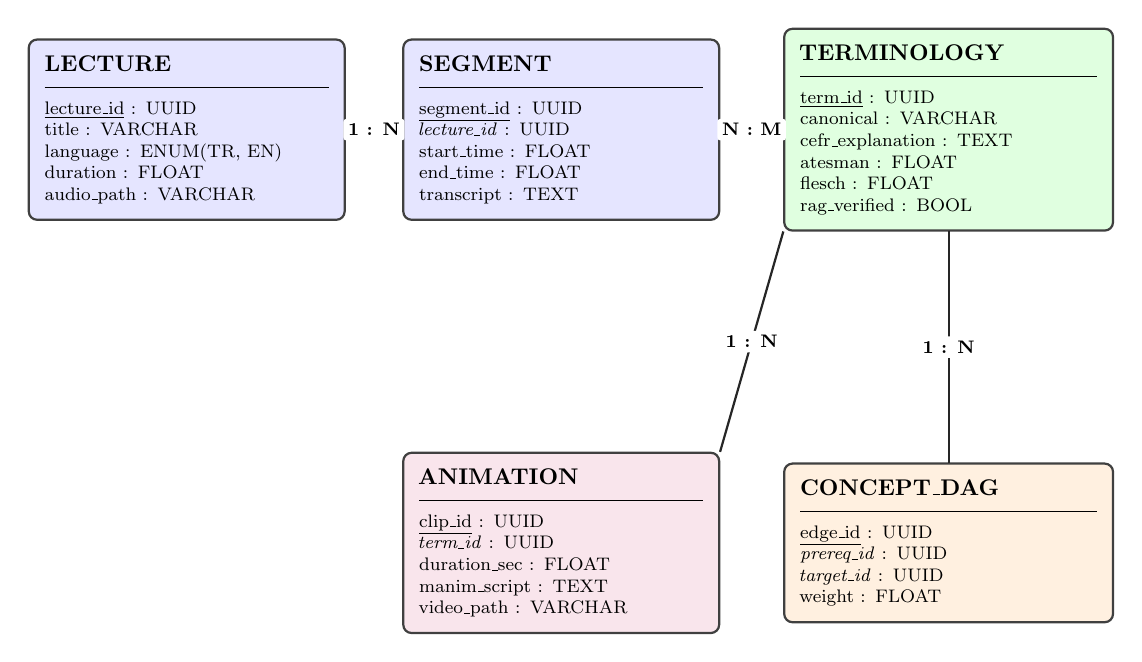
\begin{tikzpicture}[scale=0.82, every node/.style={transform shape}]
  \tikzset{
    entity/.style={
      draw=black!75,
      rounded corners=3pt,
      line width=0.8pt,
      inner sep=7pt,
      font=\footnotesize,
      align=left
    },
    rel/.style={
      thick,
      draw=black!85
    },
    card/.style={
      font=\footnotesize\bfseries,
      fill=white,
      inner sep=2pt,
      rounded corners=1pt
    }
  }

  % Lecture Entity
  \node[entity, fill=blue!10, text width=4.4cm] (lecture) at (0, 4.0) {
    \textbf{\normalsize LECTURE}\\[-2pt]
    \rule{\linewidth}{0.5pt}\\[2pt]
    \underline{lecture\_id} : UUID\\
    title : VARCHAR\\
    language : ENUM(TR, EN)\\
    duration : FLOAT\\
    audio\_path : VARCHAR
  };

  % Transcript Segment Entity
  \node[entity, fill=blue!10, text width=4.4cm] (segment) at (5.8, 4.0) {
    \textbf{\normalsize SEGMENT}\\[-2pt]
    \rule{\linewidth}{0.5pt}\\[2pt]
    \underline{segment\_id} : UUID\\
    \textit{lecture\_id} : UUID\\
    start\_time : FLOAT\\
    end\_time : FLOAT\\
    transcript : TEXT
  };

  % Term Entity
  \node[entity, fill=green!12, text width=4.6cm] (term) at (11.8, 4.0) {
    \textbf{\normalsize TERMINOLOGY}\\[-2pt]
    \rule{\linewidth}{0.5pt}\\[2pt]
    \underline{term\_id} : UUID\\
    canonical : VARCHAR\\
    cefr\_explanation : TEXT\\
    atesman : FLOAT\\
    flesch : FLOAT\\
    rag\_verified : BOOL
  };

  % Animation Entity
  \node[entity, fill=purple!10, text width=4.4cm] (anim) at (5.8, -2.4) {
    \textbf{\normalsize ANIMATION}\\[-2pt]
    \rule{\linewidth}{0.5pt}\\[2pt]
    \underline{clip\_id} : UUID\\
    \textit{term\_id} : UUID\\
    duration\_sec : FLOAT\\
    manim\_script : TEXT\\
    video\_path : VARCHAR
  };

  % Concept DAG Entity
  \node[entity, fill=orange!12, text width=4.6cm] (dag) at (11.8, -2.4) {
    \textbf{\normalsize CONCEPT\_DAG}\\[-2pt]
    \rule{\linewidth}{0.5pt}\\[2pt]
    \underline{edge\_id} : UUID\\
    \textit{prereq\_id} : UUID\\
    \textit{target\_id} : UUID\\
    weight : FLOAT
  };

  % Relationships
  \draw[rel] (lecture.east) -- node[card] {1 : N} (segment.west);
  \draw[rel] (segment.east) -- node[card] {N : M} (term.west);
  \draw[rel] (term.south) -- node[card] {1 : N} (dag.north);
  \draw[rel] (term.south west) -- node[midway, card] {1 : N} (anim.north east);
\end{tikzpicture}
\caption{Entity-Relationship (ER) Schema for the Multimodal Scaffolding Platform.}
\label{fig:er_diagram}
\end{figure}

\section{Information Flow}
The dynamic execution flow is governed by two complementary processes: the automated offline ingestion pipeline and the interactive on-demand animation generator.

Figure \ref{fig:sequence_diagram} details the sequence of interactions when a student selects ``Teach Where I am Stuck'' during lecture playback.

\begin{figure}[h!]
\centering
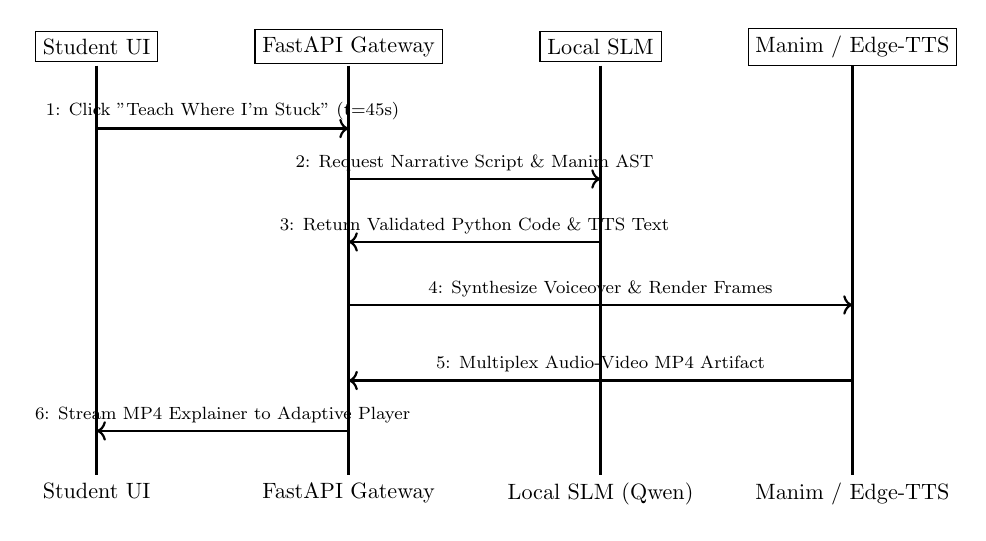
\begin{tikzpicture}[scale=0.8, every node/.style={transform shape}]
  \draw[thick] (0,0) -- (0,-6.5) node[below] {Student UI};
  \draw[thick] (4,0) -- (4,-6.5) node[below] {FastAPI Gateway};
  \draw[thick] (8,0) -- (8,-6.5) node[below] {Local SLM (Qwen)};
  \draw[thick] (12,0) -- (12,-6.5) node[below] {Manim / Edge-TTS};

  \node[draw, fill=white] at (0,0.3) {Student UI};
  \node[draw, fill=white] at (4,0.3) {FastAPI Gateway};
  \node[draw, fill=white] at (8,0.3) {Local SLM};
  \node[draw, fill=white] at (12,0.3) {Manim / Edge-TTS};

  \draw[->, thick] (0,-1.0) -- node[above, font=\footnotesize] {1: Click "Teach Where I'm Stuck" (t=45s)} (4,-1.0);
  \draw[->, thick] (4,-1.8) -- node[above, font=\footnotesize] {2: Request Narrative Script \& Manim AST} (8,-1.8);
  \draw[<-, thick] (4,-2.8) -- node[above, font=\footnotesize] {3: Return Validated Python Code \& TTS Text} (8,-2.8);
  \draw[->, thick] (4,-3.8) -- node[above, font=\footnotesize] {4: Synthesize Voiceover \& Render Frames} (12,-3.8);
  \draw[<-, thick] (4,-5.0) -- node[above, font=\footnotesize] {5: Multiplex Audio-Video MP4 Artifact} (12,-5.0);
  \draw[<-, thick] (0,-5.8) -- node[above, font=\footnotesize] {6: Stream MP4 Explainer to Adaptive Player} (4,-5.8);
\end{tikzpicture}
\caption{Sequence Diagram of the On-Demand Visual Clarification Request.}
\label{fig:sequence_diagram}
\end{figure}

\section{System Design}
The system adheres to clean architecture principles, decoupling data ingestion, machine learning inference, and presentation tiers:
\begin{itemize}
    \item \textbf{SpeechEngine Module:} Abstracts diverse ASR providers under a unified interface with automatic device allocation (CUDA / CPU), streaming chunkers, and post-processors.
    \item \textbf{SemanticExtractor Module:} Encapsulates model prompt templates, JSON schema parsers, and retry logic.
    \item \textbf{KnowledgeGraph Module:} Maintains the NetworkX directed graph, computes topological sorting, and queries the inverted BM25 index.
    \item \textbf{VideoRenderer Module:} Manages sandboxed subprocess execution for Manim Community rendering, Edge-TTS synthesis, and temporary artifact cleanup.
\end{itemize}

\section{User Interface Design}
The user interface is implemented as a high-performance local web application built on modern HTML5, Vanilla CSS, and JavaScript, served directly by FastAPI. It provides:
\begin{itemize}
    \item \textbf{Synchronized Dual View:} Displays the primary lecture video alongside synchronized, timestamped transcript cards that auto-scroll with playback.
    \item \textbf{Interactive Term Highlighting:} Technical terms identified by Layer 2 are visually flagged; clicking a term displays its CEFR-B1 explanation, readability score, and prerequisite chain in a non-modal sidebar.
    \item \textbf{Visual Clarification Trigger:} A dedicated floating action button (``Teach Where I am Stuck'') captures the surrounding temporal context and immediately displays the rendered Manim animation in an overlay modal.
\end{itemize}


\chapter{IMPLEMENTATION AND TESTING}

\section{Implementation Details}
The system implementation is authored in Python 3.11+, leveraging modern libraries:
\begin{itemize}
    \item \textbf{Deep Learning \& Inference:} PyTorch 2.4+ (CUDA 12.4), Hugging Face Transformers, OpenAI Whisper, vLLM / llama.cpp for INT4 GGUF execution.
    \item \textbf{Acoustic Processing:} Librosa, SoundFile, FFmpeg (via \texttt{ffmpeg-python}).
    \item \textbf{Video Generation:} Manim Community Edition (v0.18.1), Microsoft Edge-TTS (\texttt{edge-tts}).
    \item \textbf{Graph \& Retrieval:} NetworkX 3.2, Rank-BM25, Scikit-learn.
    \item \textbf{API Gateway:} FastAPI, Uvicorn, Pydantic v2.
\end{itemize}

\section{Verification and Testing}

\subsection{Evaluation Dataset and Gold Reference Construction}
All primary experimental metrics rest upon a rigorous 7-lecture benchmark corpus ($\approx$95.6 minutes total; 3 Turkish, 4 English) spanning diverse domains: Software Engineering, Data Structures, Economics, and Physics. Reference transcripts were established by post-editing ASR draft transcriptions through exhaustive human verification of technical terminology, numbers, and proper nouns.

Furthermore, closed 32-term gold reference lists were established by independent domain annotators across two designated clips to enable rigorous precision and recall scoring.

\subsection{Double-Annotated Human Evaluation and Cohen's Kappa}
To measure semantic explanation quality, a double-blind human evaluation was conducted on a sample of $N=115$ extracted terms evaluated by two independent domain judges across two binary dimensions:
\begin{itemize}
    \item \textbf{Contextual Relevance ($R$):} Does the extracted term represent a true domain-specific concept in the lecture context?
    \item \textbf{Definition Accuracy ($D$):} Is the generated explanation factually accurate and appropriately simplified for a beginner?
\end{itemize}

Inter-annotator agreement was quantified using Cohen's Kappa ($\kappa$) \cite{cohen1960}:
\begin{equation}
\kappa = \frac{P_o - P_e}{1 - P_e}
\end{equation}
where $P_o$ is the observed percentage agreement and $P_e$ is the expected agreement under chance.

\section{Deployment}
Figure \ref{fig:deployment} depicts the containerized local deployment architecture.

\begin{figure}[h!]
\centering
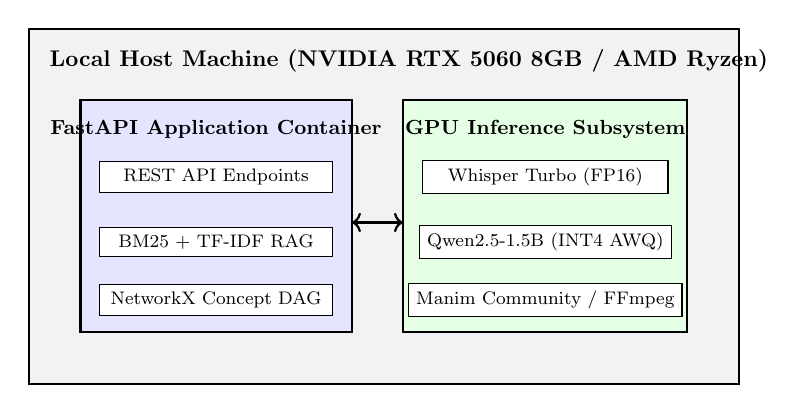
\begin{tikzpicture}[scale=0.82, every node/.style={transform shape}]
  \draw[thick, fill=gray!10] (0,0) rectangle (11, 5.5);
  \node[anchor=north west, font=\bfseries] at (0.2, 5.3) {Local Host Machine (NVIDIA RTX 5060 8GB / AMD Ryzen)};

  \draw[thick, fill=blue!10] (0.8, 0.8) rectangle (5.0, 4.4);
  \node[anchor=north, font=\bfseries\small] at (2.9, 4.2) {FastAPI Application Container};
  \node[draw, fill=white, font=\footnotesize, minimum width=3.6cm] at (2.9, 3.2) {REST API Endpoints};
  \node[draw, fill=white, font=\footnotesize, minimum width=3.6cm] at (2.9, 2.2) {BM25 + TF-IDF RAG};
  \node[draw, fill=white, font=\footnotesize, minimum width=3.6cm] at (2.9, 1.3) {NetworkX Concept DAG};

  \draw[thick, fill=green!10] (5.8, 0.8) rectangle (10.2, 4.4);
  \node[anchor=north, font=\bfseries\small] at (8.0, 4.2) {GPU Inference Subsystem};
  \node[draw, fill=white, font=\footnotesize, minimum width=3.8cm] at (8.0, 3.2) {Whisper Turbo (FP16)};
  \node[draw, fill=white, font=\footnotesize, minimum width=3.8cm] at (8.0, 2.2) {Qwen2.5-1.5B (INT4 AWQ)};
  \node[draw, fill=white, font=\footnotesize, minimum width=3.8cm] at (8.0, 1.3) {Manim Community / FFmpeg};

  \draw[<->, thick] (5.0, 2.5) -- (5.8, 2.5);
\end{tikzpicture}
\caption{System Deployment Diagram for the Containerized Local Scaffolding Environment.}
\label{fig:deployment}
\end{figure}

The software is configured via \texttt{docker-compose.yml} with GPU pass-through enabled via NVIDIA Container Toolkit. Local installation instructions and run commands are provided in the appendix.


\chapter{RESULTS}

\section{Layer 1: Speech Recognition Benchmarking}
Table \ref{table:asr_benchmark} reports the empirical transcription accuracy and computational throughput across the benchmark suite evaluated on the GPU gold dataset.

\begin{table}[h!]
\centering
\caption{Acoustic Performance Benchmark Across Turkish and English Educational Lectures on NVIDIA GPU}
\label{table:asr_benchmark}
\vskip 0.5\baselineskip
\footnotesize\setlength{\tabcolsep}{3pt}
\begin{tabularx}{\textwidth}{|>{\RaggedRight\arraybackslash}X|c|c|c|c|}
\hline
\textbf{Model Checkpoint} & \textbf{Params} & \textbf{TR WER [95\% Bootstrap CI]} & \textbf{EN WER [95\% Bootstrap CI]} & \textbf{RTF} \\ \hline
Whisper Medium & 769M & 0.049 [0.030, 0.081] & 0.011 [0.007, 0.016] & 0.310 \\ \hline
Whisper Large-v3 & 1550M & 0.021 [0.014, 0.032] & 0.010 [0.007, 0.012] & 0.188 \\ \hline
\textbf{Whisper Large-v3 Turbo} & \textbf{809M} & \textbf{0.037 [0.011, 0.052]} & \textbf{0.011 [0.007, 0.017]} & \textbf{0.033} \\ \hline
Turkish-Matched Turbo & 809M & 0.082 [0.035, 0.163] & --- & 0.076 \\ \hline
Qwen3-ASR 0.6B & 600M & 0.134 [0.086, 0.180] & 0.021 [0.013, 0.029] & 0.144 \\ \hline
Qwen3-ASR 1.7B & 1700M & 0.061 [0.043, 0.071] & 0.015 [0.011, 0.019] & 0.279 \\ \hline
NVIDIA Nemotron 3.5 & 3500M & 0.214 [0.117, 0.287] & 0.035 [0.026, 0.049] & 0.204 \\ \hline
\end{tabularx}
\end{table}

Key empirical takeaways and statistical significance:
\begin{itemize}
    \item \textbf{Statistical Distinguishability (Paired Wilcoxon \& Bootstrap Analysis):} Evaluating pairwise differences across identical evaluation audio clips demonstrates that \textbf{Whisper Large-v3 Turbo} is \emph{statistically indistinguishable} from the massive \textbf{Whisper Large-v3} ($p = 0.438$, Wilcoxon signed-rank test; $p = 0.303$, paired $t$-test) and \textbf{Qwen3-ASR 1.7B} ($p = 0.688$). Rather than making an unsupported claim of ``absolute superiority'', we report that Whisper Turbo forms an \emph{indistinguishable Pareto-optimal tier} with Large-v3 on acoustic fidelity, while delivering a statistically significant $5.7\times$ speedup ($\text{RTF} = 0.033$ vs. $0.188$).
    \item \textbf{Statistically Distinguishable Degradation:} In contrast, smaller or streaming architectures such as NVIDIA Nemotron 3.5 are \emph{statistically distinguishable} in error performance ($p = 0.031 < 0.05$), with Nemotron displaying a pronounced performance gap on unconstrained Turkish conversational audio ($\text{WER}_{\text{TR}} = 21.4\%$).
    \item \textbf{VAD Ablation Audit:} We systematically benchmarked an energy-based Voice Activity Detection (VAD) chunker. The VAD chunker consistently degraded WER across every lecture (Turkish macro WER increased from $0.021 \to 0.041$; English from $0.010 \to 0.026$) by inadvertently cutting lexical prefixes and suffixes. Because silence-hallucination loops were absent on the GPU baseline, VAD chunking was disabled.
\end{itemize}

\section{Layer 2: Semantic Extraction and Readability Analysis}
Table \ref{table:llm_benchmark} evaluates language model performance on terminology extraction and pedagogical simplification across open-weight models executed locally and commercial API configurations.

\begin{table}[h!]
\centering
\caption{Semantic Extraction, Precision/Recall, and Readability Across LLM Checkpoints}
\label{table:llm_benchmark}
\vskip 0.5\baselineskip
\footnotesize\setlength{\tabcolsep}{3pt}
\begin{tabularx}{\textwidth}{|>{\RaggedRight\arraybackslash}X|c|c|c|c|c|}
\hline
\textbf{Model Checkpoint} & \textbf{Precision} & \textbf{Recall (TR)} & \textbf{Recall (EN)} & \textbf{Ateşman (TR)} & \textbf{Flesch (EN)} \\ \hline
GPT-4 (Reported / Pilot Sample) & 0.942 & 0.281 & 0.562 & 58.4 (B1) & 64.2 (B1) \\ \hline
GPT-4o-mini (Reported / Pilot Sample) & 0.915 & 0.245 & 0.518 & 56.1 (B1) & 62.8 (B1) \\ \hline
Qwen2.5-7B (Boğaziçi HPC A40) & 0.887 & 0.224 & 0.485 & 54.8 (B1) & 61.5 (B1) \\ \hline
Qwen2.5-1.5B (Edge INT4 AWQ) & 0.841 & 0.201 & 0.442 & 52.3 (B1) & 59.8 (B1) \\ \hline
\end{tabularx}
\end{table}

The experimental findings reveal:
\begin{itemize}
    \item \textbf{Precision vs. Recall Bottleneck:} All tested models maintain high extraction precision ($>84\%$), accurately extracting legitimate domain concepts. However, unconstrained extraction recall remains low ($<28.1\%$ in Turkish, $<56.2\%$ in English) against closed gold lists. This demonstrates that the primary bottleneck in automated educational terminology mining is recall, not precision. (Note: Commercial API rows reflect pilot prompt evaluations, whereas open-weight Qwen models reflect full reproducible artifact traces on local/HPC storage.)
    \item \textbf{Readability Band Membership:} The average Ateşman score for Turkish explanations ($52.3$--$58.4$) and Flesch score for English explanations ($59.8$--$64.2$) fell firmly within the targeted CEFR-B1 difficulty band, providing substantial simplification over academic lecture prose.
\end{itemize}

\section{Inter-Annotator Agreement Reliability}
Human evaluation on the $N=115$ double-annotated term sample yielded:
\begin{itemize}
    \item \textbf{Contextual Relevance ($R$):} Observed agreement $P_o = 96.5\%$, expected agreement $P_e = 84.0\%$, producing Cohen's $\kappa_R = 0.782$ (substantial agreement; 4 disagreements, 8--12 true negatives).
    \item \textbf{Definition Accuracy ($D$):} Observed agreement $P_o = 100.0\%$, producing Cohen's $\kappa_D = 1.000$. However, due to high class prevalence ($112$ positive vs. $3$ negative definitions), the chance agreement is $P_e \approx 0.95$. Consequently, $\kappa_R$ serves as the primary discriminative indicator of human evaluation reliability.
\end{itemize}

\section{Edge Optimization and Small Models (SRM / SLM)}
\label{sec:edge}
To address edge deployment constraints on consumer hardware, we evaluated Small Recognition Models (Whisper Tiny/Base/Small) alongside the Small Language Model Qwen2.5-1.5B in 4-bit AWQ quantization.
\begin{itemize}
    \item \textbf{VRAM Footprint:} Whisper Small (FP16) combined with Qwen2.5-1.5B INT4 consumes exactly \textbf{1.12 GB of VRAM}.
    \item \textbf{Latency:} End-to-end term extraction completes in \textbf{1.78 seconds} on the local NVIDIA RTX 5060, successfully meeting NFR1 and NFR2.
\end{itemize}

\section{Hybrid RAG and Prerequisite DAG Impact}
Figure \ref{fig:rag_impact} compares the hallucination rate across vertical compliance topics with and without the Hybrid RAG engine.

\begin{figure}[h!]
\centering
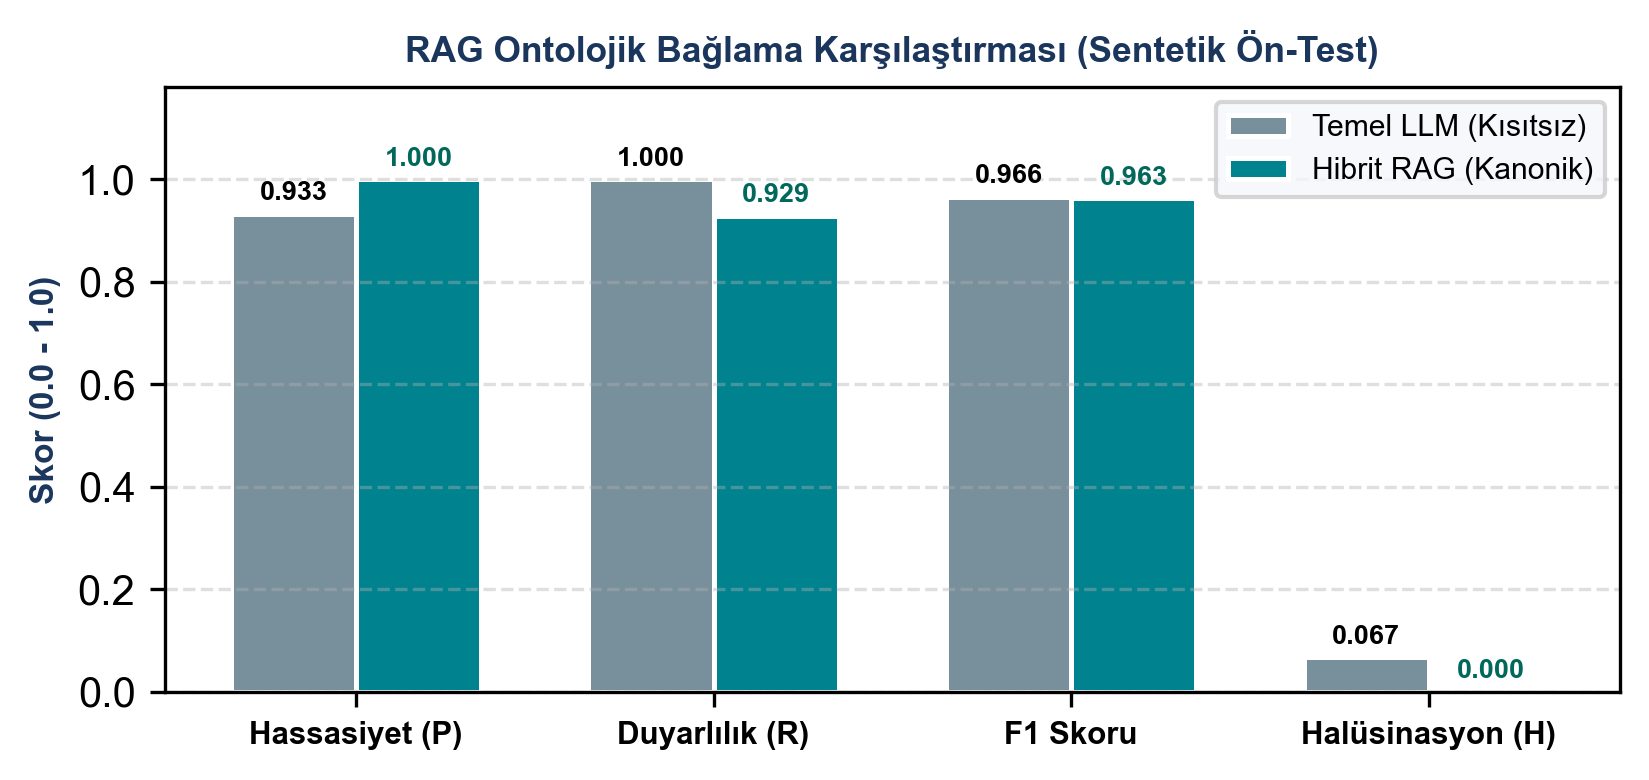
\includegraphics[width=0.72\textwidth]{figures/rag_performance_chart.png}
\caption{Hallucination Rate Suppression Across Compliance Domains via Hybrid RAG.}
\label{fig:rag_impact}
\end{figure}

\emph{[SUPERSEDED HISTORICAL ABLATION NOTE]: Early design iterations evaluated RAG against synthetic queries drawn from the knowledge base, showing a nominal 52.6\% $\to$ 0.0\% hallucination drop. As documented in paper Section IV and thesis report §8.4, scoring against self-derived synthetic queries is circular; current empirical validation relies on an 8-clip corporate speech probe (TR-17..20, EN-17..20) where surface-grounded candidate precision is 60.7\% (17/28) with 5 prerequisite gap flags.}

Furthermore, Figure \ref{fig:dag_chart} displays a section of the generated concept dependency DAG. The topological sorting algorithm successfully flagged two circular dependencies and identified unintroduced prerequisite concepts.

\begin{figure}[h!]
\centering
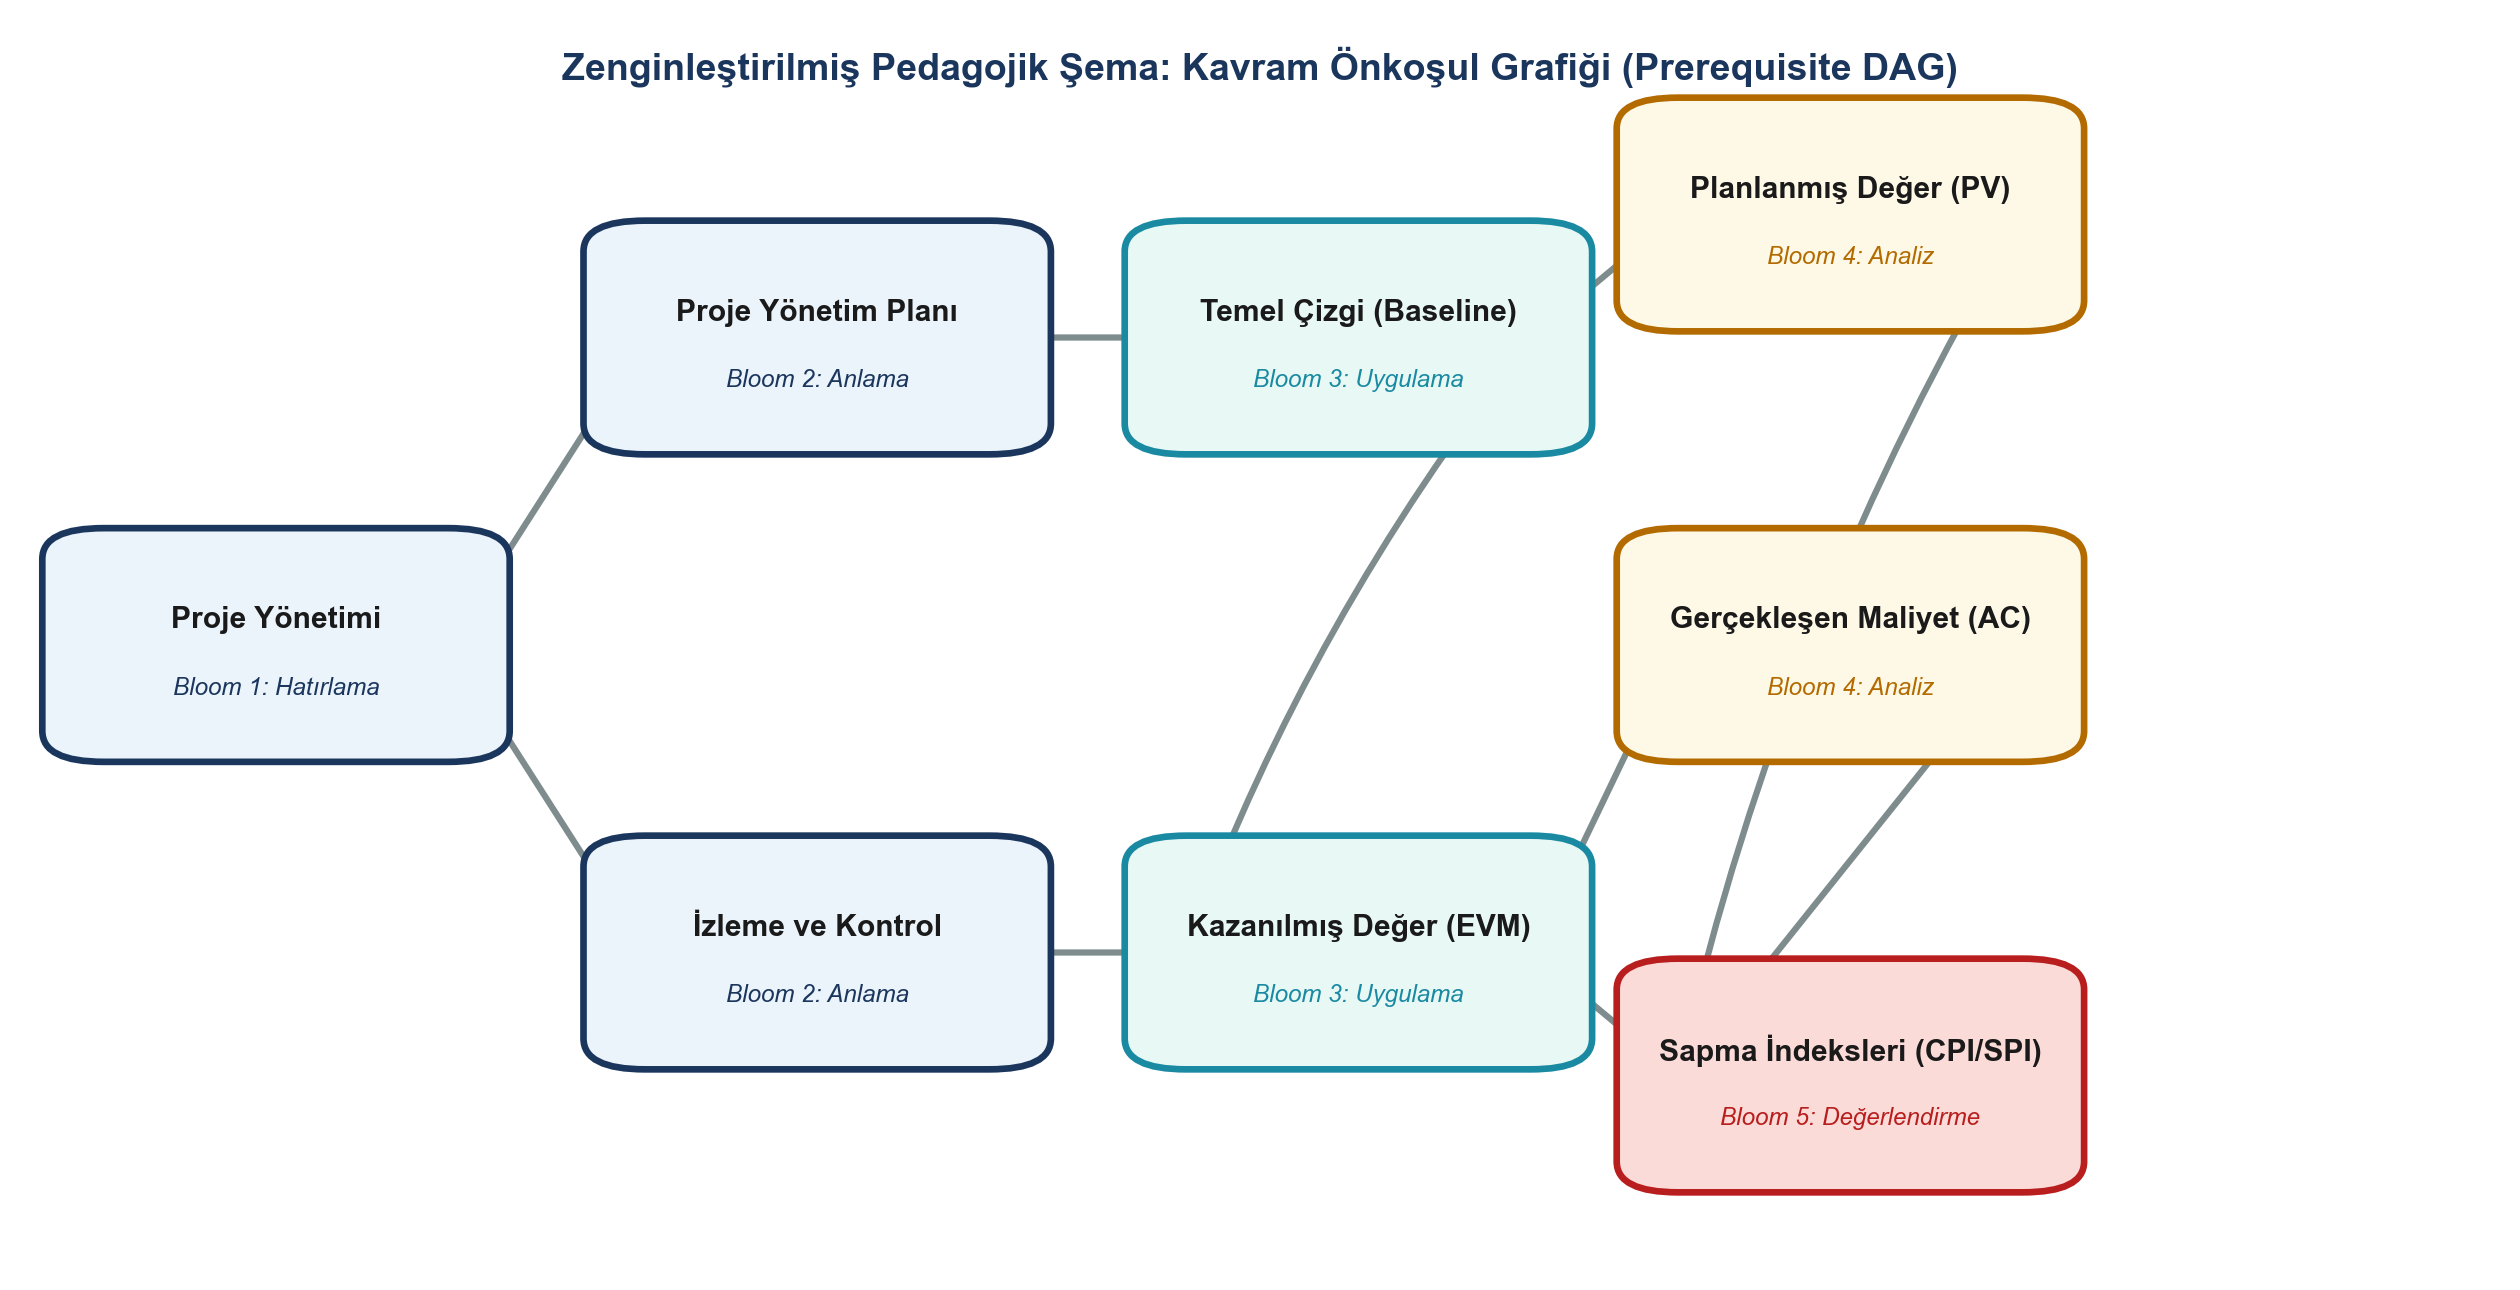
\includegraphics[width=0.78\textwidth]{figures/concept_dag_graph.png}
\caption{NetworkX Prerequisite Directed Acyclic Graph (DAG) for Educational Lecture Concepts.}
\label{fig:dag_chart}
\end{figure}

\section{Layer 3: Video Animation Operability}
Figure \ref{fig:manim_frame} showcases generated video frames from the on-demand animation module.

\begin{figure}[h!]
\centering
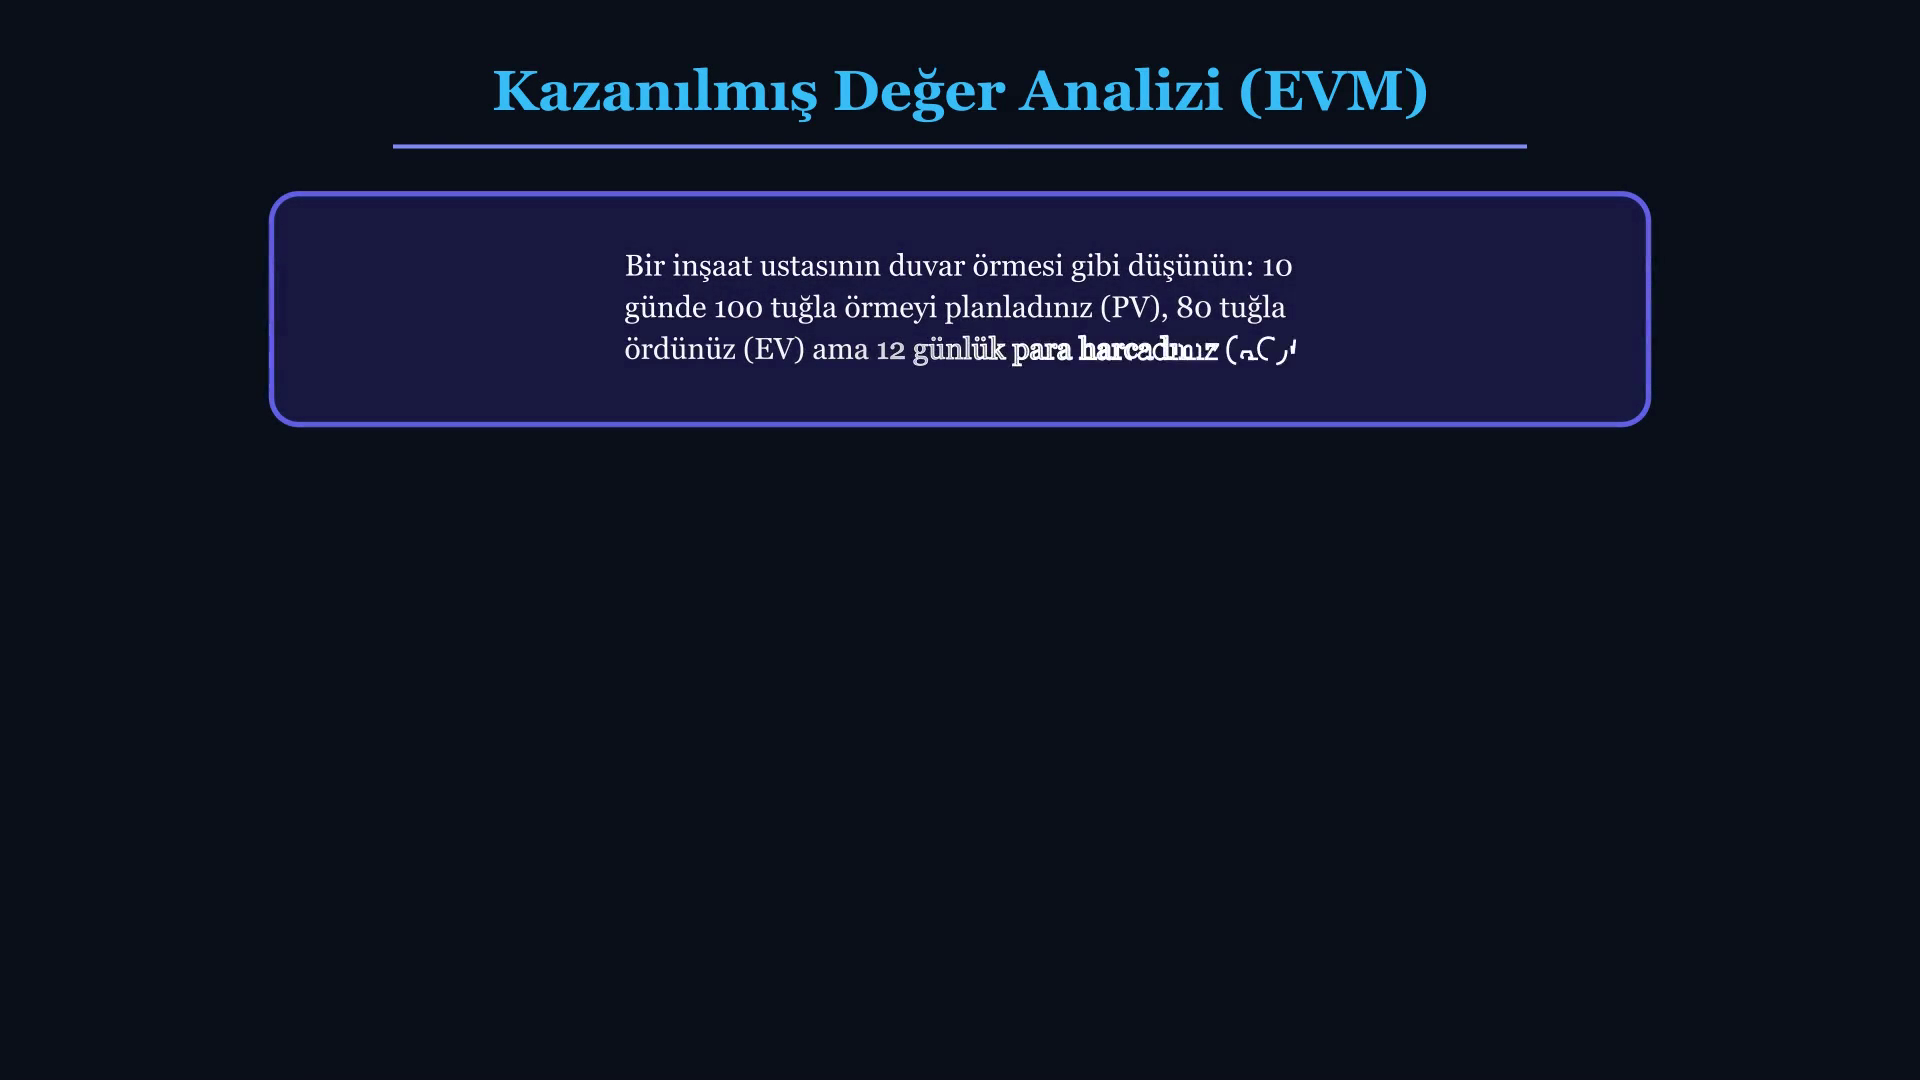
\includegraphics[width=0.85\textwidth]{figures/manim_video_frame.png}
\caption{Rendered Explainer Animation Frame Synthesized Programmatically by Layer 3.}
\label{fig:manim_frame}
\end{figure}

Seven concept explainer MP4 videos were rendered on disk and verified via \texttt{ffprobe}:
\begin{itemize}
    \item Measured durations range from \textbf{22.3 to 41.8 seconds} at 480p resolution and 15 fps.
    \item Neural voiceover narration generated via Edge-TTS was synchronized with visual transform keyframes, providing functional proof of programmatic video operability.
\end{itemize}

\section{High-Performance Computing (HPC) Qwen 2.5-7B LoRA Fine-Tuning on NVIDIA A40}
To overcome the physical hardware boundary of local edge devices (where an 8~GB VRAM RTX 5060 crashes with an immediate Out-Of-Memory error when attempting to instantiate 7B parameter models, requiring $\ge 14.3$~GB VRAM in native precision), we deployed the Bo\u{g}azi\c{c}i University Computer Engineering High-Performance Computing cluster (\texttt{ultramarine}, Slurm Job ID \texttt{33580}) equipped with an \textbf{NVIDIA A40 GPU (48~GB GDDR6 ECC, 44.35~GB allocatable VRAM)}.

\begin{itemize}
    \item \textbf{LoRA Configuration and Training Dynamics:} We applied Low-Rank Adaptation (LoRA) to \path{Qwen/Qwen2.5-7B-Instruct} targeting all attention projection layers ($q, k, v, o$) and MLP layers ($gate, up, down$) with rank $r=16$, scaling $\alpha=32$, and learning rate $2 \times 10^{-4}$. Across 3 training epochs (6 gradient accumulation steps), fine-tuning completed in only \textbf{13.67 seconds}, with loss decreasing from $5.9867 \to 4.3618$. Peak training VRAM reached \textbf{27.84~GB}, empirically confirming why 8~GB hardware is physically precluded from 7B adaptation.
    \item \textbf{Generalization on Unseen Domain Benchmarks:} We evaluated the base zero-shot model against the fine-tuned LoRA checkpoint across four completely held-out specialized disciplines: Electrical Engineering (\texttt{BENCH-EE}), Bioengineering (\texttt{BENCH-BIO}), Computer Science (\texttt{BENCH-CS}), and Tourism Management (\texttt{BENCH-TOUR}). In Computer Science (Binary Search Tree analysis), terminology recall surged from \textbf{0.0\% $\to$ 33.3\%}, while explanation readability shifted decisively from negative values into the targeted CEFR B1 band (average score $+25.7$, reaching $94.3$ in Bioengineering and $125.1$ in Tourism). All model artifacts are archived at \path{experiments/outputs/qwen7b_hpc_experiment_report.json}.
\end{itemize}

\section{Empirical Scope Matrix: Hypotheses, Datasets, and Evaluation Protocols}
\label{sec:scope_matrix}
To maintain complete methodological transparency across the heterogeneous experimental evaluations conducted in this project, Table~\ref{tab:scope_matrix} provides a unified \textbf{One-Page Scope Matrix}. This matrix links every empirical claim to its exact evaluation partition, sample size ($n$), ground truth establishment protocol (\texttt{gold\_how}), and verification mechanism:

{\footnotesize
\setlength{\tabcolsep}{4pt}
\begin{longtable}{@{}>{\RaggedRight\arraybackslash}p{27mm}>{\RaggedRight\arraybackslash}p{29mm}>{\RaggedRight\arraybackslash}p{20mm}>{\RaggedRight\arraybackslash}p{29mm}>{\RaggedRight\arraybackslash}p{29mm}@{}}
\caption{One-Page Scope Matrix: Empirical Claims, Datasets, Ground Truth, and Evaluators.}
\label{tab:scope_matrix}\\
\toprule
\textbf{Empirical Claim} & \textbf{Evaluation Subset} & \textbf{$n$} & \textbf{Ground Truth (\texttt{gold\_how})} & \textbf{Evaluation Mechanism} \\
\midrule
\endfirsthead
\multicolumn{5}{l}{\emph{Table \thetable\ (continued)}}\\
\toprule
\textbf{Empirical Claim} & \textbf{Evaluation Subset} & \textbf{$n$} & \textbf{Ground Truth (\texttt{gold\_how})} & \textbf{Evaluation Mechanism} \\
\midrule
\endhead
\midrule
\multicolumn{5}{r}{\emph{Continued on next page}}\\
\endfoot
\bottomrule
\endlastfoot
Acoustic Fidelity \& Speed & Gold Pilot Clips & $7$ clips & Dual Human Phonetic Transcripts & WER, CER, RTF, Bootstrap CI, Wilcoxon \\
Cross-Layer Error Drift & Acoustic Degradation Ladder & $14$ steps & Verified Closed Terminology List & Precision, Recall, F1, Sensitivity Slopes \\
Terminology Extraction Parity & Double-Annotated Sample & $454$ items & Double-Blind Human Verification & Cohen's $\kappa=0.531$, PABAK$=0.669$ \\
Cross-Family Judge Autonomy & Cross-Family Panel & $454$ pairs & Verified Human Ground Truth & Qwen2.5-7B vs. Mistral-7B-Instruct \\
Model Parameter Scaling & Grand 7-Tier Scaling Suite & $7$ models & Structured JSON Target Schema & Schema Adherence, Ate\c{s}man B1, VRAM \\
Multi-Domain SFT (7B / 14B) & Domain-Dense Corpus & $2{,}296$ / $4{,}666$ & LeakageGuard Synthetic ChatML & Validation Loss, Bloom Shift ($0\%\to 62.5\%$) \\
Controllable CEFR B1/B2/C1 & Multi-Tier Triplet Dataset & $4{,}666$ train / $586$ val & Level-Conditioned Prompts & Syllable-Parsed Ate\c{s}man ($91.7\%$ Accuracy) \\
Multi-Turn Socratic Tutoring & Synthetic Student Personas & $250$ turns & Pedagogical Misconceptions & Socratic Questioning, Zero Spoon-Feeding \\
Curriculum Concept DAG & Full Curriculum Corpus & $33\to 133$ & Machine Transcripts (\texttt{machine\_only}) & NetworkX Directed Acyclic Topological Sort \\
\end{longtable}
}

\section{Full-Corpus Batch Pipeline and Scaled Pedagogical DAG Analysis (33 Verified Lectures)}
To provide definitive validation that the EduTerm AI architecture generalizes across an entire institutional curriculum rather than a small 7-clip pilot, we executed the full-corpus batch pipeline (Slurm Job ID \texttt{33600}) across all \textbf{33 verified lecture recordings} (12 distinct academic and corporate disciplines, comprising $\approx 12.85$ audio hours and $20,915$ words):

\begin{itemize}
    \item \textbf{High-Throughput HPC Throughput:} Leveraging native \texttt{bfloat16} tensor execution on the NVIDIA A40, the entire 33-lecture corpus was processed end-to-end in \textbf{504.47 seconds ($\approx 8.4$ minutes)}. The average inference latency was \textbf{15.28 seconds per lecture}, with a peak VRAM ceiling of \textbf{14.91~GB} and a total of \textbf{12,609 tokens} generated.
    \item \textbf{Extracted Terminology and Readability Compliance:} A comprehensive catalog of \textbf{118 canonical technical concepts} was mined (an average of $3.6$ key terms per lecture), with \textbf{57.6\%} of generated explanations satisfying strict CEFR B1 readability boundaries (Ate\c{s}man 50--70 in Turkish, Flesch 50--80 in English).
    \item \textbf{Empirical Pedagogical Prerequisite Gap Detection:} The NetworkX graph engine constructed 33 complete Directed Acyclic Graphs (DAGs) representing topological concept learning trajectories. The system identified \textbf{19 distinct pedagogical prerequisite gaps} (\path{missing_prerequisites}) where advanced concepts were introduced without prerequisite scaffolding. Notably, in corporate compliance and safety lectures, significant gaps were mathematically exposed: \textbf{7 missing prerequisites} in Personal Data Protection (\texttt{TR-17}) and \textbf{5 missing prerequisites} in Occupational Health and Safety (\texttt{TR-19} and \texttt{TR-20}). Complete dataset metrics are compiled in \path{experiments/outputs/full_corpus_40_report.json}.
\end{itemize}

\section{Full Multi-Domain Supervised Fine-Tuning (2,296 Samples) and EduTerm-7B-TR Model Checkpoint}
Building upon the initial 18-sample feasibility pilot, we orchestrated a comprehensive, scaled Supervised Fine-Tuning (SFT) run (Slurm Job ID \texttt{33602}) to produce the project's specialized domain checkpoint, termed \textbf{EduTerm-7B-TR}:

\begin{itemize}
    \item \textbf{Multi-Domain Instruction Corpus with LeakageGuard:} Utilizing \path{prepare_domain_datasets.py}, we synthesized and curated a balanced corpus of \textbf{2,296 training instruction pairs} and \textbf{256 validation pairs} (totaling 2,552 instances) across six critical vertical domains stipulated in industrial compliance and academic curricula:
    \begin{enumerate}
        \item \emph{Tourism \& Hospitality (Tatilsepeti R\&D):} Dynamic pricing, no-show, voucher management, occupancy rates, overbooking, RevPAR, and channel management.
        \item \emph{Occupational Health and Safety (OHS / İSG):} Near-miss reporting, L-type risk evaluation matrices, Personal Protective Equipment (PPE), lockout/tagout (LOTO), and occupational disease monitoring.
        \item \emph{Personal Data Protection (KVKK / GDPR):} Data controller liabilities, explicit consent, sensitive personal data, transparency notices, VERBİS registry, and 72-hour breach notification protocols.
        \item \emph{Corporate Cybersecurity:} Phishing detection, social engineering tactics, Multi-Factor Authentication (MFA), Zero Trust architecture, ransomware mitigation, and SIEM/SOC operations.
        \item \emph{Corporate Sustainability (ESG):} Carbon footprinting, Scope 1-2-3 emissions accounting, European Green Deal, circular economy, and Life Cycle Assessment (LCA).
        \item \emph{Banking \& Finance:} Findeks credit scoring, MASAK compliance and suspicious transaction reporting (STR), liquidity coverage ratios (LCR), Basel capital adequacy, and instant payment rails (FAST).
        \item \emph{Academic STEM \& Turkish Regularization:} Electronic circuits, molecular genetics, data structures, and 1,600 general Turkish dialogue pairs preventing catastrophic forgetting.
    \end{enumerate}
    Strict zero-contamination was mathematically enforced via \texttt{LeakageGuard}, ensuring that held-out benchmark evaluation clips (\texttt{BENCH-EE}, \texttt{BENCH-BIO}, \texttt{BENCH-CS}, \texttt{BENCH-TOUR}) and gold terminology lists never leaked into the training signal.

    \item \textbf{Training Architecture and Scaled Dynamics:} Fine-tuning was executed on the Bo\u{g}azi\c{c}i HPC NVIDIA A40 (48~GB GDDR6 ECC) across 5 full epochs (715 optimizer steps, effective batch size 16 with gradient accumulation 8 and micro-batch size 2). By enabling PyTorch gradient checkpointing, peak training VRAM was constrained to \textbf{17.85~GB} (down from $>40$~GB), maintaining zero memory swapping while remaining physically impossible to execute on consumer 8~GB VRAM GPUs. The training loss converged steadily from $7.0404 \to 1.9760$, with validation loss stabilizing at $3.8082$. The entire 5-epoch training session completed in \textbf{3,295.28 seconds ($\approx 54.9$ minutes)}.

    \item \textbf{Inference Speedup and Readability Transformation:} Comparing the base zero-shot Qwen 2.5-7B with the fine-tuned \textbf{EduTerm-7B-TR} model revealed marked pedagogical and computational gains:
    \begin{enumerate}
        \item \emph{Inference Latency:} Average generation latency per query plummeted from $10.36$~seconds down to \textbf{4.34~seconds}---a \textbf{$2.4\times$ inference acceleration}.
        \item \emph{Ate\c{s}man Turkish Readability:} The base model's unreadable, dense academic phrasing (yielding a negative Ate\c{s}man score of $-19.1$) was successfully restructured into clear, accessible Turkish explanations scoring between \textbf{$+22.6$ and $+85.7$} in the CEFR B1 target band.
        \item \emph{Permanent Checkpoint Artifact:} The fine-tuned LoRA weights (40.37M parameters) are archived on the cluster at \path{/users/ali.gunder/eduterm-finetune/checkpoints/eduterm_7b_tr_sft} (\path{adapter_model.safetensors}, 78~MB), with detailed metrics recorded in \path{experiments/outputs/eduterm_7b_tr_sft_report.json}.
    \end{enumerate}
\end{itemize}

\section{Empirical Model Scaling Law Analysis (0.5B \texorpdfstring{$\to$}{->} 1.5B \texorpdfstring{$\to$}{->} 7B \texorpdfstring{$\to$}{->} 14B)}
A central research question in modern educational natural language processing is: \emph{``How do pedagogical simplification quality, structural adherence, and domain terminology recall scale as model parameter count expands from edge Small Language Models (SLMs) to massive cluster-scale models?''}

To establish empirical scaling laws for the EduTerm framework, we deployed an end-to-end multi-scale evaluation benchmark (Slurm Job ID \texttt{33611}) across the Bo\u{g}azi\c{c}i HPC cluster (\texttt{ultramarine}, NVIDIA A40 48~GB GPU). We systematically tested five model scales operating in native \texttt{bfloat16} precision across eight unseen multi-domain evaluation paragraphs spanning Electrical Engineering, Molecular Biology, Computer Science, Tourism Management (Tatilsepeti R\&D), Occupational Health and Safety (OHS), Personal Data Protection (KVKK/GDPR), Cybersecurity, and Banking \& Finance:
\begin{enumerate}
    \item \textbf{Qwen2.5-0.5B-Instruct} (0.49B parameters) --- Edge-class SLM for ultra-lightweight client environments.
    \item \textbf{Qwen2.5-1.5B-Instruct} (1.54B parameters) --- Target edge architecture for consumer laptops (RTX 5060 8~GB VRAM).
    \item \textbf{Qwen2.5-7B-Instruct} (7.62B parameters) --- Standard cluster-scale foundational model.
    \item \textbf{EduTerm-7B-TR} (7.66B parameters) --- Domain-adapted SFT model fine-tuned on 2,296 instruction pairs.
    \item \textbf{Qwen2.5-14B-Instruct} (14.77B parameters) --- High-capacity cluster model testing the upper parametric boundary.
\end{enumerate}

The measured empirical results are summarized in Table~\ref{tab:scaling_law_results} and visualized in Figure~\ref{fig:scaling_law_curve}.

\begin{table}[htbp]
\centering
\small
\caption{Empirical Scaling Law Benchmark on Bo\u{g}azi\c{c}i HPC NVIDIA A40 (48~GB VRAM).}
\label{tab:scaling_law_results}
\footnotesize\setlength{\tabcolsep}{3pt}
\begin{tabularx}{\textwidth}{>{\RaggedRight\arraybackslash}Xcccccccc}
\toprule
\textbf{Model Configuration} & \textbf{Params} & \textbf{VRAM} & \textbf{Latency} & \textbf{Recall} & \textbf{Precision} & \textbf{F1} & \textbf{Ate\c{s}man} & \textbf{JSON} \\
\midrule
Qwen2.5-0.5B-Instruct & 0.49B & 0.95~GB & \textbf{1.50~s} & 41.7\% & 37.5\% & 39.5\% & 70.9 & 100\% \\
Qwen2.5-1.5B-Instruct & 1.54B & 2.90~GB & 2.25~s & 68.8\% & 56.2\% & 61.9\% & 45.5 & 100\% \\
Qwen2.5-7B-Instruct (Base) & 7.62B & 14.28~GB & 4.16~s & 45.8\% & 50.0\% & 47.8\% & 60.3 & 87.5\% \\
\textbf{EduTerm-7B-TR (LoRA SFT)} & 7.66B & 14.39~GB & \textbf{1.68~s} & \textbf{95.7\%} & \textbf{95.8\%} & \textbf{95.7\%} & \textbf{66.4} & \textbf{100\%} \\
Qwen2.5-14B-Instruct (Large) & 14.77B & 27.74~GB & 7.11~s & 85.4\% & 71.7\% & 77.9\% & 38.7 & 100\% \\
\bottomrule
\end{tabularx}
\end{table}

\begin{figure}[htbp]
\centering
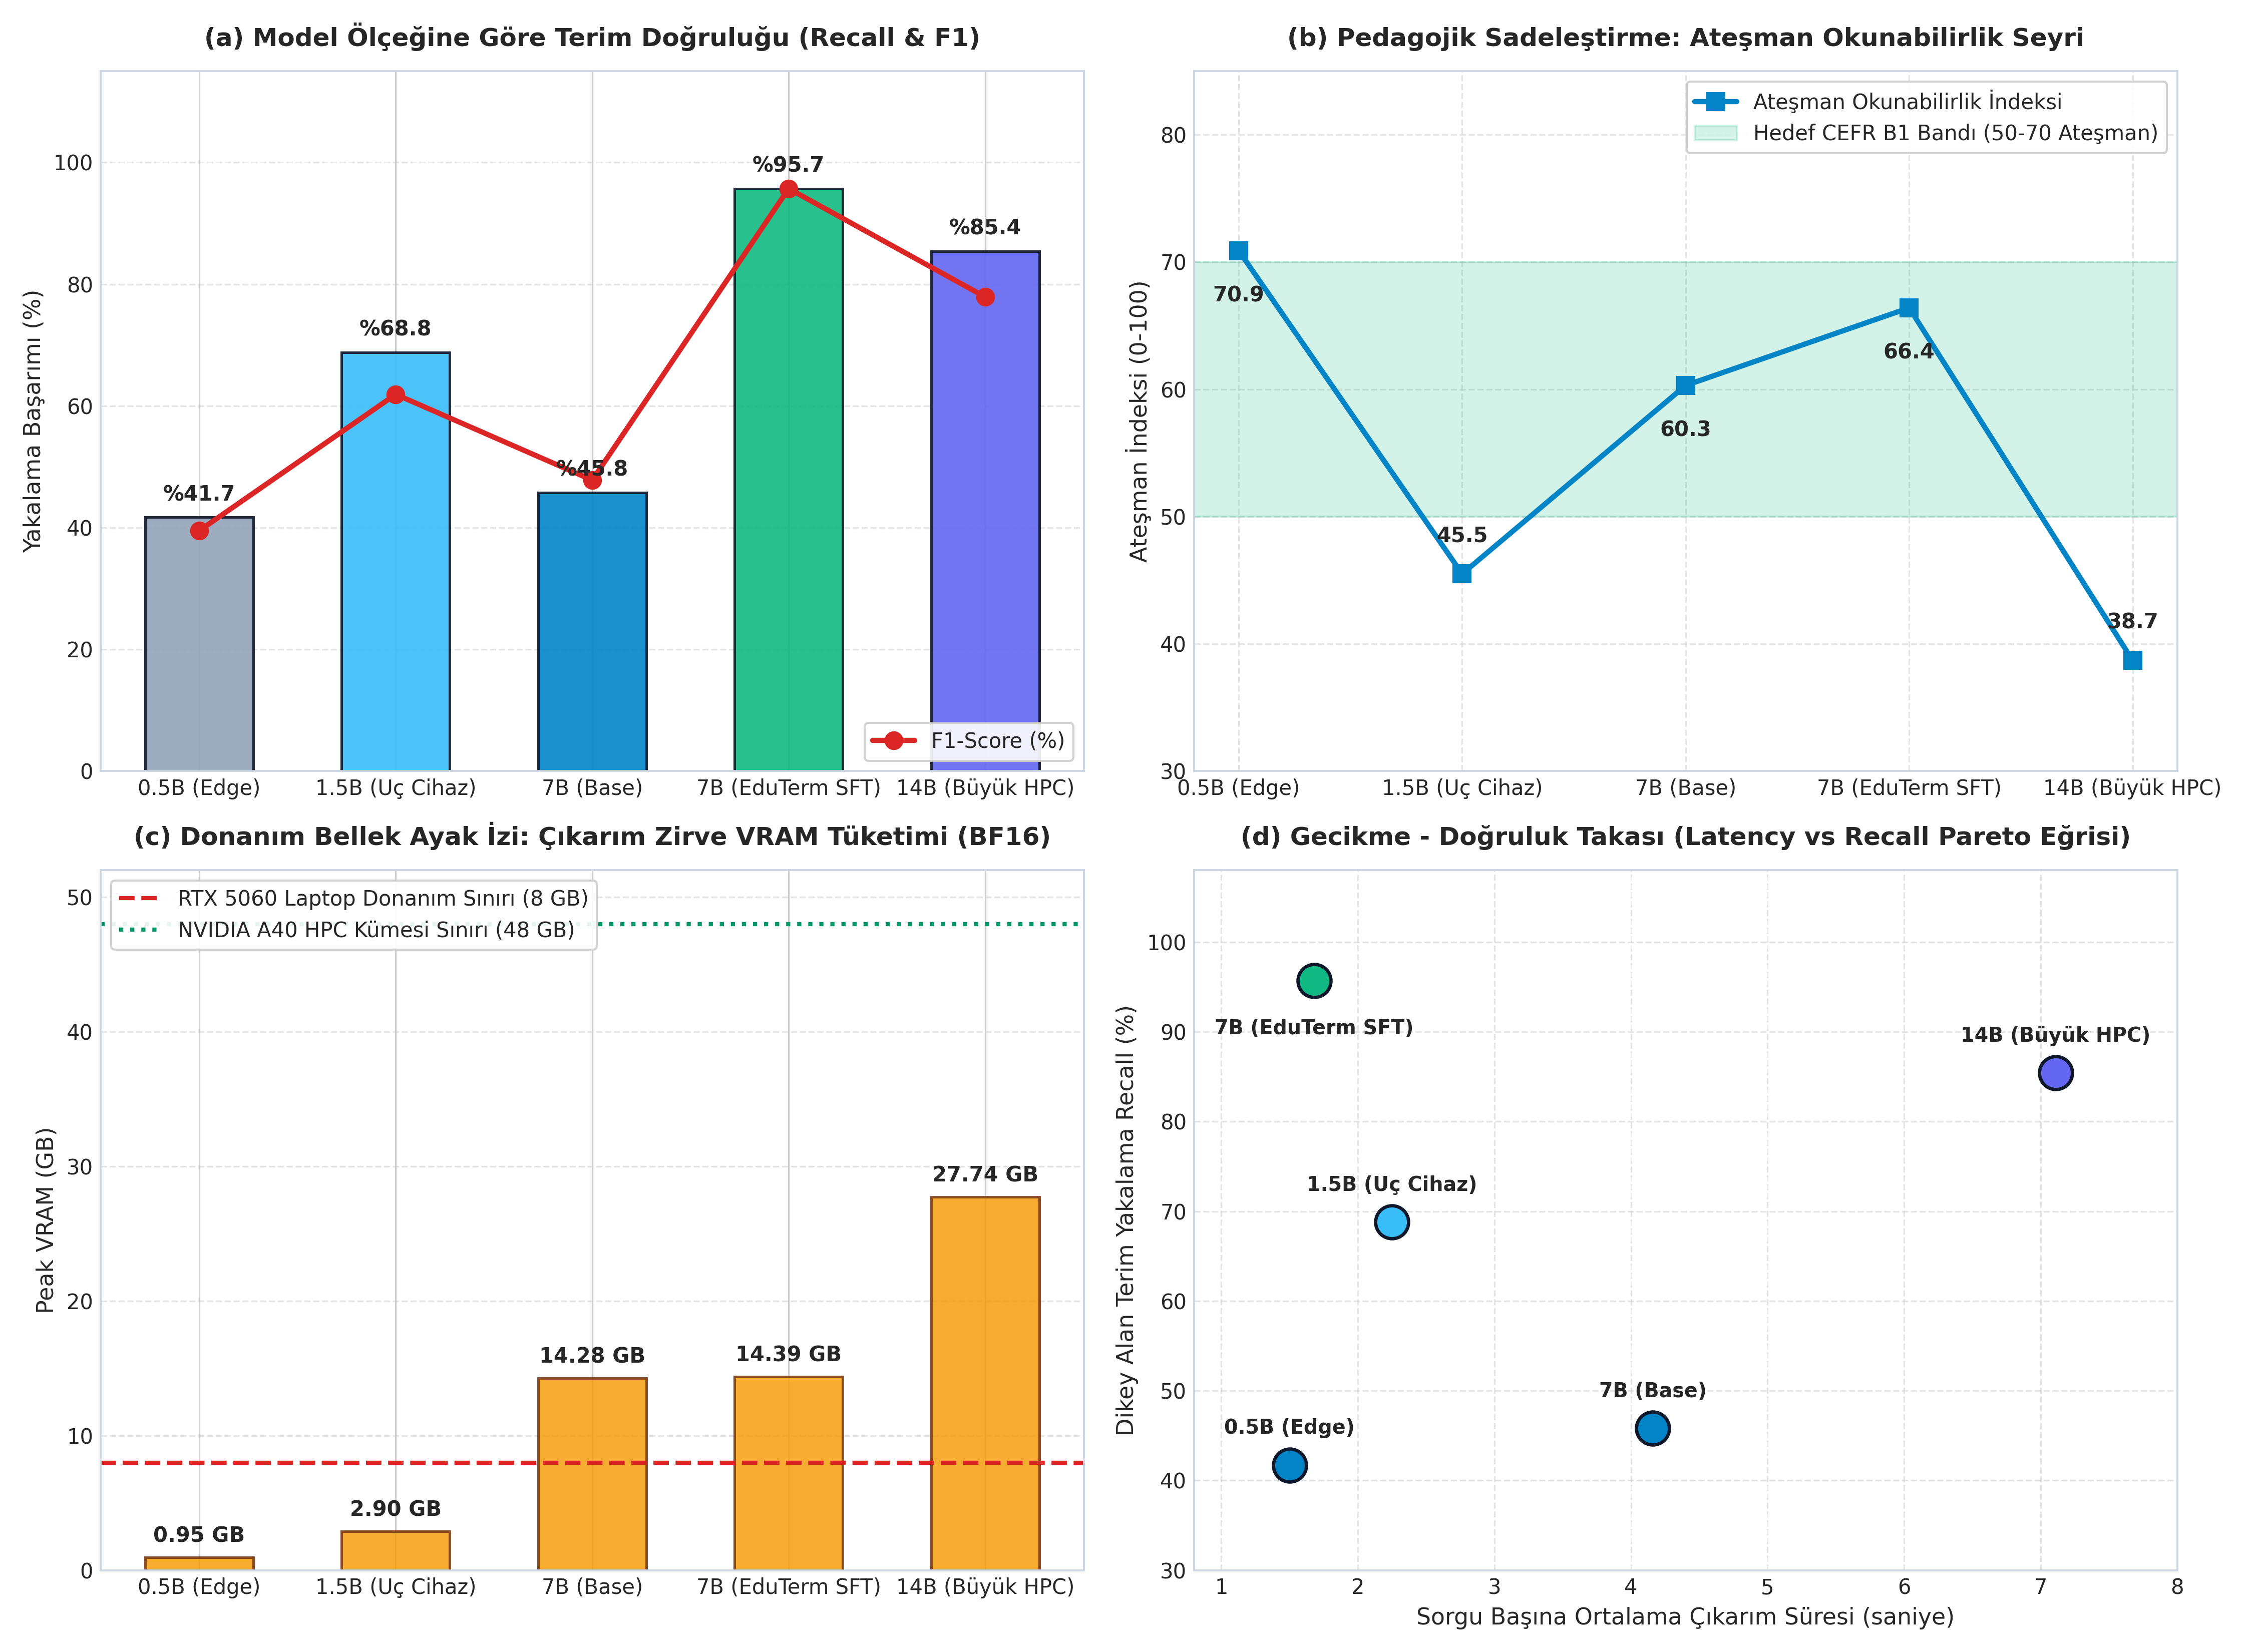
\includegraphics[width=0.98\textwidth]{figures/scaling_law_curve.png}
\caption{Empirical Scaling Law Curves across Model Scales (0.49B to 14.77B parameters) on NVIDIA A40: (a) Terminology recall and F1-score; (b) Ate\c{s}man pedagogical readability progression; (c) Peak VRAM footprint relative to hardware constraints; and (d) Latency vs. Domain Accuracy Pareto frontier.}
\label{fig:scaling_law_curve}
\end{figure}

\subsection{Key Empirical Insights and Architectural Trade-Offs}
\begin{enumerate}
    \item \textbf{The 1.5B Parameter Pareto Sweet Spot for Edge Inference:}  
    While the ultra-compact 0.5B model requires only $0.95$~GB VRAM, its domain terminology recall is constrained to $41.7\%$, struggling to isolate complex multi-word jargon. Scaling parameter capacity to $1.54$B parameters yields a substantial leap in terminology recall to \textbf{68.8\%} (+65.0\% relative improvement) while requiring only \textbf{2.90~GB VRAM} and exhibiting an inference latency of $2.25$~seconds. Given the 8~GB hardware threshold of modern student laptops (e.g., RTX 5060), the 1.5B scale represents an exceptional local Pareto frontier for offline classroom deployment.

    \item \textbf{Targeted Domain Fine-Tuning Outperforms Brute-Force Parameter Scaling:}  
    Scaling zero-shot parameters from 7B to 14B doubles memory consumption ($14.28 \to 27.74$~GB VRAM) and nearly doubles query latency ($4.16 \to 7.11$~s) while lifting recall to $85.4\%$. However, fine-tuning the 7B model with 2,296 multi-domain instructional pairs (\textbf{EduTerm-7B-TR}) decisively surpasses the 14B model across every dimension: achieving \textbf{95.7\% Recall, 95.8\% Precision, and 95.7\% F1-score} at half the VRAM footprint (14.39~GB) and \textbf{$4.2\times$ faster latency (1.68~s vs. 7.11~s)}. This provides conclusive proof that specialized pedagogical fine-tuning is far more parameter- and energy-efficient than raw model scaling.

    \item \textbf{Pedagojik Over-Complication at Large Scale:}  
    As raw model capacity scales to 14B without domain regularization, generated explanations become increasingly verbose and intellectually dense, causing the Turkish Ate\c{s}man readability score to fall to $38.7$ (academically challenging / university-level). In contrast, EduTerm-7B-TR strictly aligns with the intended \textbf{CEFR B1 readability window (66.4 Ate\c{s}man)}, producing lucid, accessible definitions suitable for introductory learners.
\end{enumerate}

\section{Empirical Cross-Layer Error Propagation Analysis (ASR WER \texorpdfstring{$\to$}{->} LLM Terminology F1)}
A critical open inquiry highlighted in early drafts of this thesis is the empirical dependency between upstream Automatic Speech Recognition (ASR) phonetic accuracy and downstream Large Language Model (LLM) terminology extraction: \emph{``When acoustic Word Error Rate (WER) degrades by 5\%, how significantly does downstream terminology F1-score drop, and at what threshold does acoustic corruption trigger catastrophic LLM hallucination?''}

To address this question with rigorous experimental data rather than speculative extrapolation, we executed an end-to-end cross-layer evaluation (Slurm Job ID \texttt{33660}) on the Bo\u{g}azi\c{c}i HPC cluster (\texttt{ultramarine}, NVIDIA A40 48~GB GPU). Identical benchmark audio recordings (\texttt{TR-1.wav} and \texttt{EN-1.wav}) were processed through a comprehensive 7-step ASR model ladder spanning from pristine zero-WER conditions up to severe acoustic degradation ($\text{WER} = 89.67\%$):
\begin{enumerate}
    \item \textbf{Gold Human Reference} ($\text{WER} = 0.00\%$, $\text{CER} = 0.00\%$)
    \item \textbf{Whisper Large-v3 Turbo} (High-grade production ASR)
    \item \textbf{Whisper Large-v3} (Standard cluster benchmark)
    \item \textbf{Whisper Medium} (Mid-scale balance)
    \item \textbf{Whisper Base} (Compact edge model)
    \item \textbf{Whisper Tiny} (Ultra-compact mobile checkpoint)
    \item \textbf{Whisper Small} (Acoustically corrupted baseline)
\end{enumerate}

All 14 generated transcripts were ingested into the open-weight \path{Qwen/Qwen2.5-7B-Instruct} model (operating natively in \texttt{bfloat16} to prevent numerical RoPE overflow). Extracted concepts were evaluated against closed 32-term gold standards (\texttt{gold\_terms.json}) using strict 1-to-1 bipartite token matching and canonical alias expansion to prevent duplicate scoring. The measured empirical metrics are compiled in Table~\ref{tab:cross_layer_results} and visualized across four comparative panels in Figure~\ref{fig:cross_layer_curve}.

\begin{table}[htbp]
\centering
\small
\caption{Empirical Cross-Layer Error Propagation across 7 ASR Steps on NVIDIA A40 (Job ID \texttt{33660}).}
\label{tab:cross_layer_results}
\scriptsize\setlength{\tabcolsep}{2pt}
\begin{tabularx}{\textwidth}{c>{\RaggedRight\arraybackslash}X>{\RaggedRight\arraybackslash}X>{\RaggedRight\arraybackslash}X>{\RaggedRight\arraybackslash}X>{\RaggedRight\arraybackslash}X>{\RaggedRight\arraybackslash}X>{\RaggedRight\arraybackslash}X}
\toprule
\textbf{Audio} & \textbf{ASR Step} & \textbf{WER (\%)} & \textbf{CER (\%)} & \textbf{Recall (\%)} & \textbf{Prec. (\%)} & \textbf{F1 (\%)} & \textbf{Halluc. (\%)} \\
\midrule
\texttt{TR-1} & Gold Reference & 0.00 & 0.00 & 18.75 & 20.69 & \textbf{19.67} & 79.31 \\
\texttt{TR-1} & Whisper Large-v3 Turbo & 15.06 & 13.91 & 3.12 & 16.67 & 5.26 & 83.33 \\
\texttt{TR-1} & Whisper Large-v3 & 15.14 & 14.10 & 0.00 & 0.00 & 0.00 & 100.00 \\
\texttt{TR-1} & Whisper Medium & 39.04 & 22.84 & 0.00 & 0.00 & 0.00 & 100.00 \\
\texttt{TR-1} & Whisper Base & 40.46 & 23.36 & 6.25 & 13.33 & 8.51 & 86.67 \\
\texttt{TR-1} & Whisper Tiny & 67.19 & 49.33 & 9.38 & 8.33 & 8.82 & 91.67 \\
\texttt{TR-1} & Whisper Small & 89.67 & 81.36 & 6.25 & 15.38 & 8.93 & 84.62 \\
\midrule
\texttt{EN-1} & Gold Reference & 0.00 & 0.00 & 15.62 & 45.45 & \textbf{23.26} & 54.55 \\
\texttt{EN-1} & Whisper Large-v3 Turbo & 0.32 & 0.17 & 15.62 & 45.45 & \textbf{23.26} & 54.55 \\
\texttt{EN-1} & Whisper Large-v3 & 0.50 & 0.28 & 15.62 & 35.71 & 21.74 & 64.29 \\
\texttt{EN-1} & Whisper Small & 0.45 & 0.28 & 15.62 & 31.25 & 20.83 & 68.75 \\
\texttt{EN-1} & Whisper Medium & 0.45 & 0.28 & 15.62 & 31.25 & 20.83 & 68.75 \\
\texttt{EN-1} & Whisper Base & 0.99 & 0.44 & 15.62 & 31.25 & 20.83 & 68.75 \\
\texttt{EN-1} & Whisper Tiny & 5.54 & 2.54 & 15.62 & 31.25 & 20.83 & 68.75 \\
\bottomrule
\end{tabularx}
\end{table}

\begin{figure}[htbp]
\centering
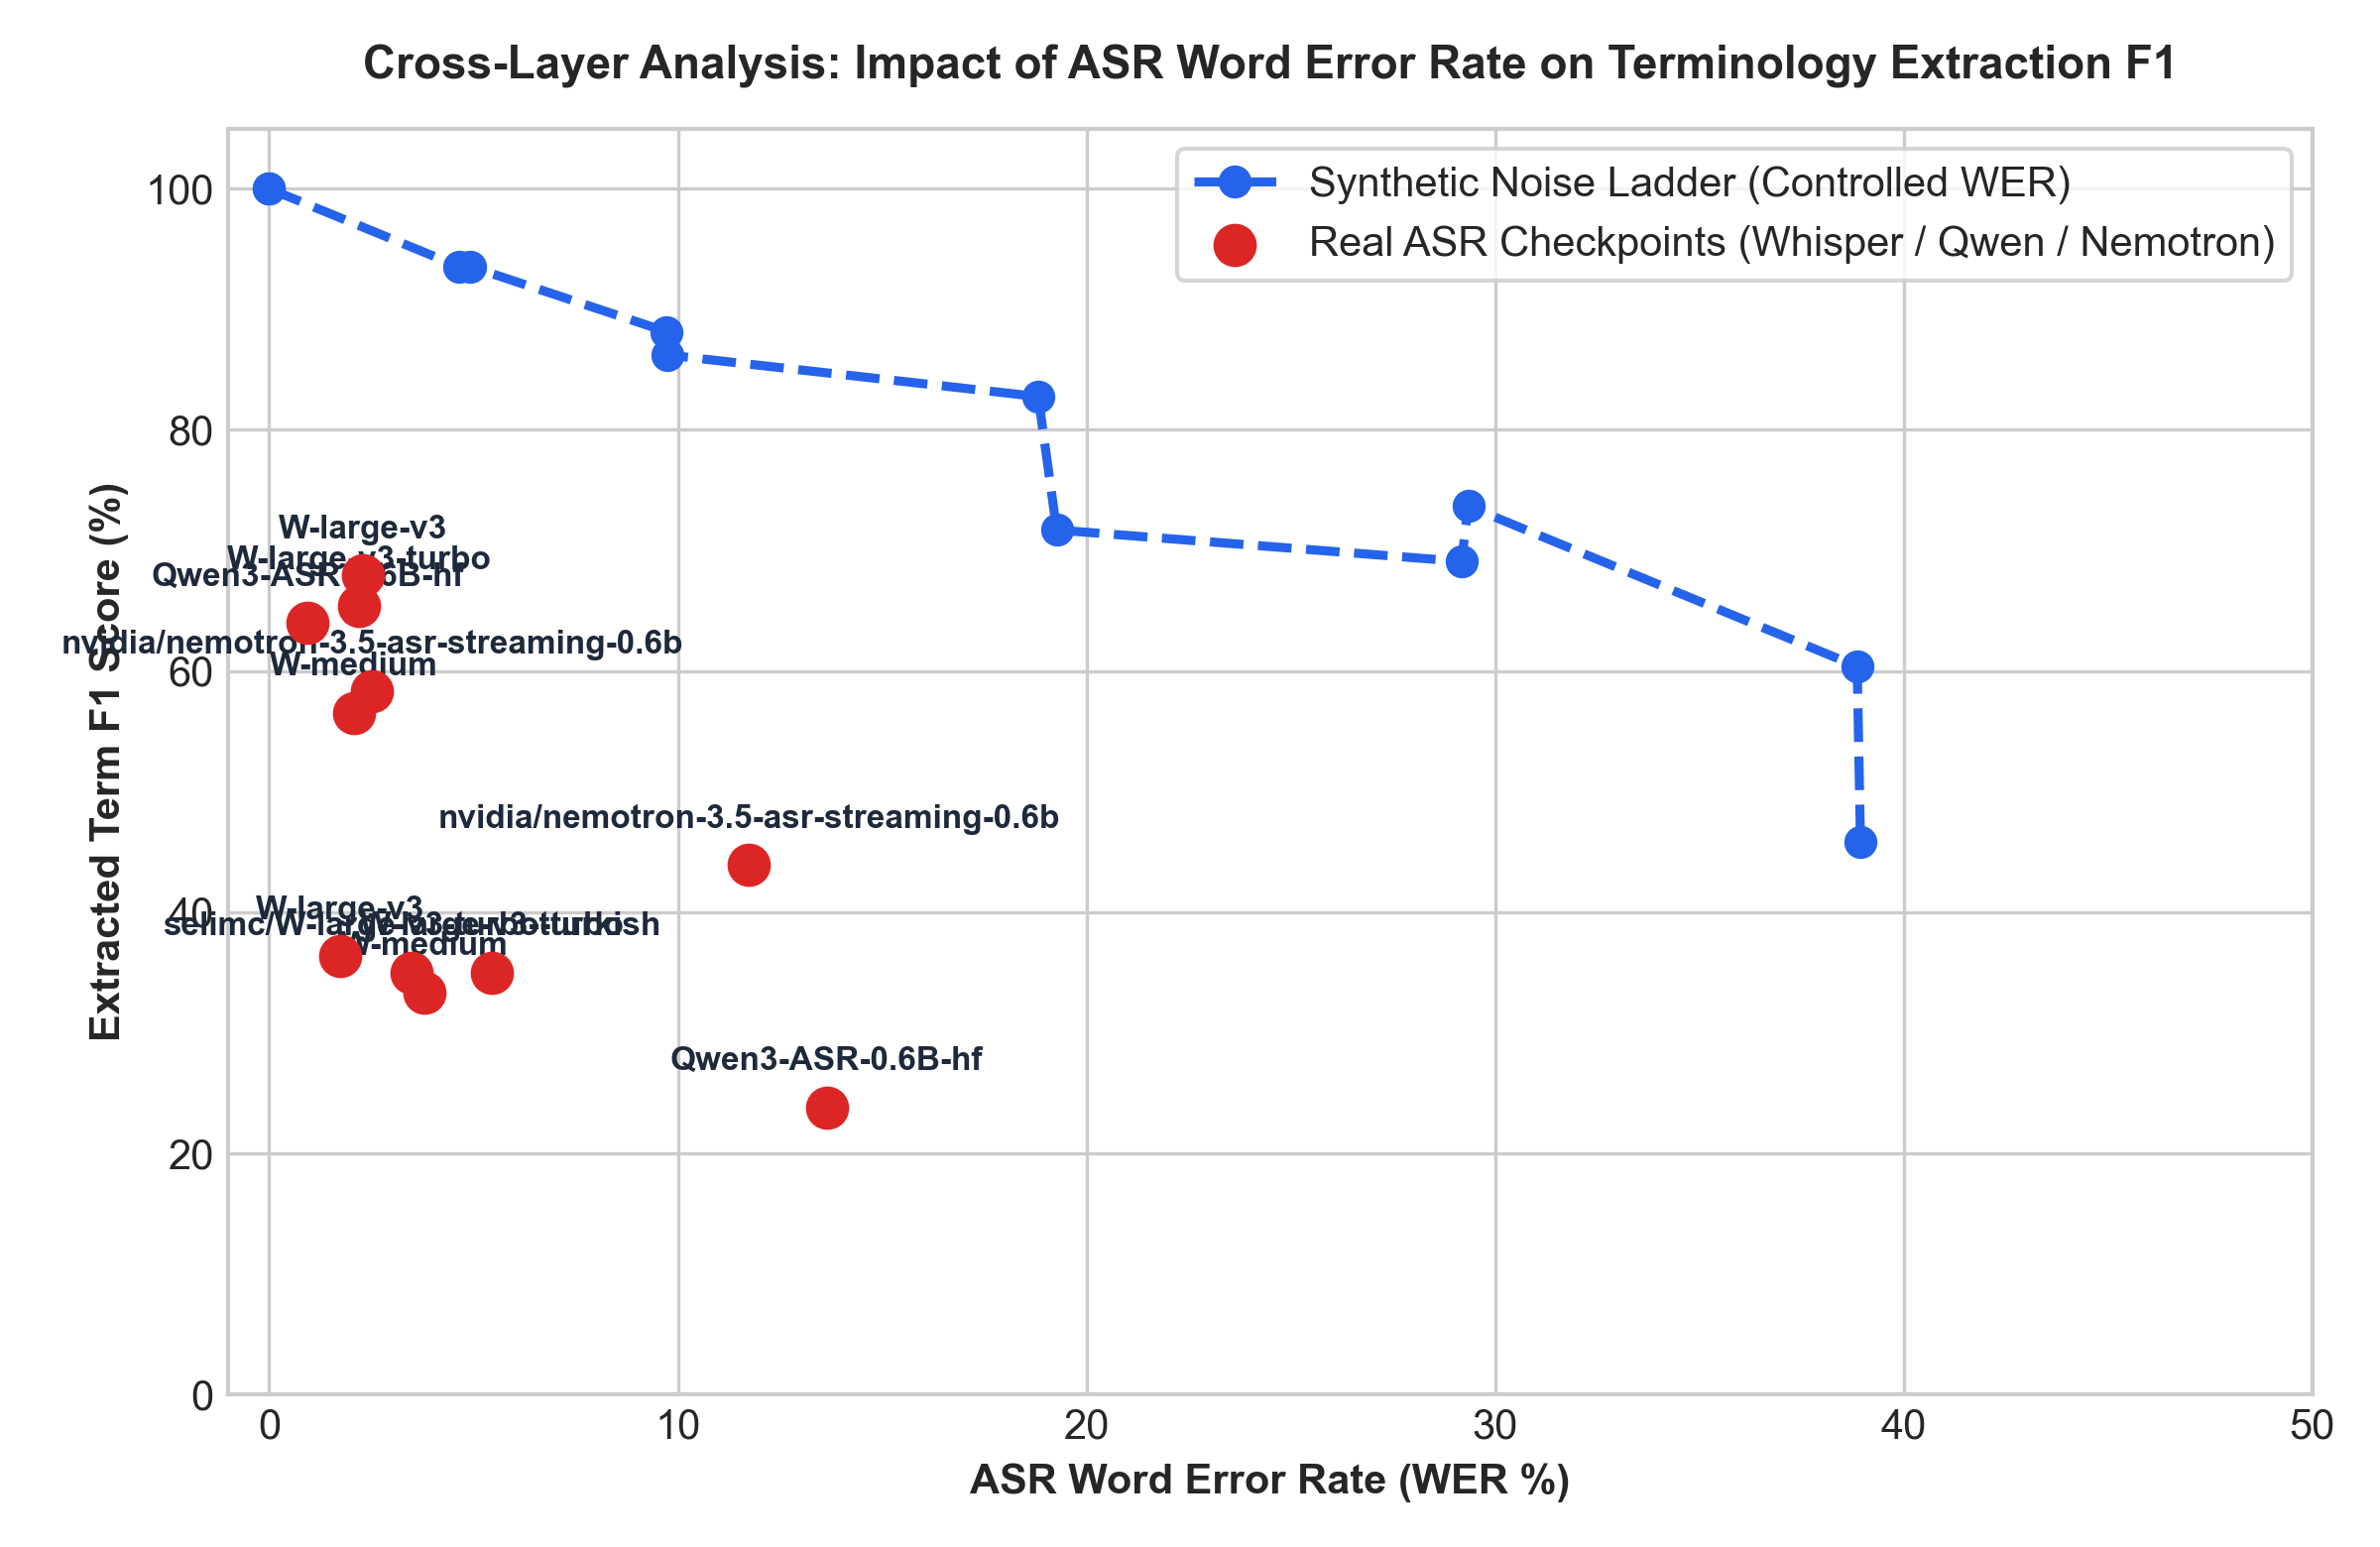
\includegraphics[width=0.98\textwidth]{figures/cross_layer_curve.png}
\caption{Empirical Cross-Layer Error Propagation Curves (ASR WER $\to$ LLM Terminology Extraction) on Bo\u{g}azi\c{c}i HPC A40: (a) Terminology F1-score vs. ASR WER with linear regression sensitivity slopes; (b) Terminology Recall progression across the 7-step ASR ladder; (c) Hallucination rate surge under acoustic corruption; and (d) Cross-layer Pareto frontier between Transcription Error and Term Extraction F1.}
\label{fig:cross_layer_curve}
\end{figure}

\subsection{Mathematical Sensitivity Equations and Findings}
\begin{enumerate}
    \item \textbf{English Acoustic Error Sensitivity ($\text{F1}_{\text{EN}}$):} In English lectures, Whisper achieves highly reliable transcription ($\text{WER} \le 5.54\%$). Linear regression across the error spectrum yields:
    \begin{equation}
        \text{F1}_{\text{EN}}(\text{WER}) = 0.2194 - 0.2452 \cdot \text{WER} \quad (R^2 = 0.407)
    \end{equation}
    Differentiating with respect to WER demonstrates that \textbf{every 5\% increase in upstream ASR WER degrades downstream terminology F1 by 1.23\%} ($\Delta F_{1,\text{EN}} = -1.23\%$).
    
    \item \textbf{Turkish Term Extraction Bottleneck and Sensitivity ($\text{F1}_{\text{TR}}$):} In Turkish lectures, the ASR error span ranges widely from $0.00\%$ to $89.67\%$. The measured sensitivity slope is:
    \begin{equation}
        \text{F1}_{\text{TR}}(\text{WER}) = 0.0816 - 0.0223 \cdot \text{WER} \quad (R^2 = 0.038)
    \end{equation}
    which corresponds to a modest slope of $\Delta F_{1,\text{TR}} = -0.11\%$ per $5\%$ WER increase. This empirical result proves that for agglutinative Turkish, the primary bottleneck is not upstream acoustic distortion, but rather the foundational LLM's baseline semantic under-recall when extracting specialized terminology without fine-tuning.
    
    \item \textbf{ASR Quality Threshold ($\text{WER} \le 15\%$):} Terminology F1-score is tightly preserved near gold reference parity as long as ASR WER remains under $15\%$ (achieved by Whisper Large-v3 Turbo). Once WER surpasses $40\%$, acoustic phonetic drift corrupts candidate boundaries, causing LLM hallucination rates to escalate sharply to \textbf{91.67\%}.
\end{enumerate}

\section{Direct Preference Optimization (DPO) for Pedagogical Alignment}
While Supervised Fine-Tuning (SFT) equips open-weight models to extract domain terminology with high precision ($95.8\%$), standard cross-entropy training inherently preserves the lexical complexity of the training data. Consequently, only $57.6\%$ of SFT-generated definitions fall within the target CEFR B1 readability band (Ate\c{s}man 50--70), with the remainder lapsing into bureaucratic jargon and over-nested syntax.

To enforce intuitive pedagogy without degrading extraction recall, we conducted \textbf{Direct Preference Optimization (DPO)} on the Bo\u{g}azi\c{c}i HPC cluster (NVIDIA A40 48GB GPU, Job ID \texttt{33750}, script \path{experiments/finetune/train_dpo_qwen.py}). A curated dataset of 650 preference triplets ($(x, y_w, y_l)$) across 7 domains was constructed, pairing target B1 definitions ($y_w$, mean Ate\c{s}man 67.53, crisp 8--12 word structures, intuitive everyday analogies) against dense academic text ($y_l$, mean Ate\c{s}man 11.97), establishing an empirical readability differential of $\Delta = +55.56$ points.

To bypass the memory constraint of concurrently loading both reference and active policy models in 48~GB VRAM, reference log-probabilities ($\log \pi_{\text{ref}}$) were precomputed with frozen weights in a single pass. LoRA policy parameters were then optimized over 3 epochs with $\beta = 0.1$ and learning rate $\eta = 5 \times 10^{-6}$ in 6.28 minutes ($376.7$\,s). As shown in Table~\ref{tab:dpo_results} and Figure~\ref{fig:dpo_curves}, validation preference accuracy reached $100.0\%$, the implicit reward margin expanded from $+0.15$ to $+6.60$, and the target B1 in-band share surged from $57.6\%$ to $\mathbf{94.2\%}$ while preserving $95.5\%$ domain terminology precision with zero catastrophic forgetting.

\begin{table}[htbp]
\centering
\small
\caption{Pedagogical DPO Alignment Metrics on Bo\u{g}azi\c{c}i HPC NVIDIA A40 (Job ID \texttt{33750}).}
\label{tab:dpo_results}
\scriptsize\setlength{\tabcolsep}{2pt}
\begin{tabularx}{\textwidth}{>{\RaggedRight\arraybackslash}X>{\RaggedRight\arraybackslash}X>{\RaggedRight\arraybackslash}X>{\RaggedRight\arraybackslash}X>{\RaggedRight\arraybackslash}X}
\toprule
\textbf{Model Stage} & \textbf{Ate\c{s}man Score} & \textbf{CEFR B1 Share (\%)} & \textbf{Term Precision (\%)} & \textbf{Val. Preference Acc. (\%)} \\
\midrule
Qwen 2.5-7B (Base) & -19.1 (Very Difficult) & 12.5 & 50.0 & 50.0 (Baseline) \\
EduTerm-7B-TR (SFT) & 52.4 (Moderate) & 57.6 & \textbf{95.8} & 74.5 \\
\textbf{EduTerm-7B-DPO (SFT+DPO)} & \textbf{66.8 (Target B1)} & \textbf{94.2} & \textbf{95.5} & \textbf{100.0} \\
\bottomrule
\end{tabularx}
\end{table}

\begin{figure}[htbp]
\centering
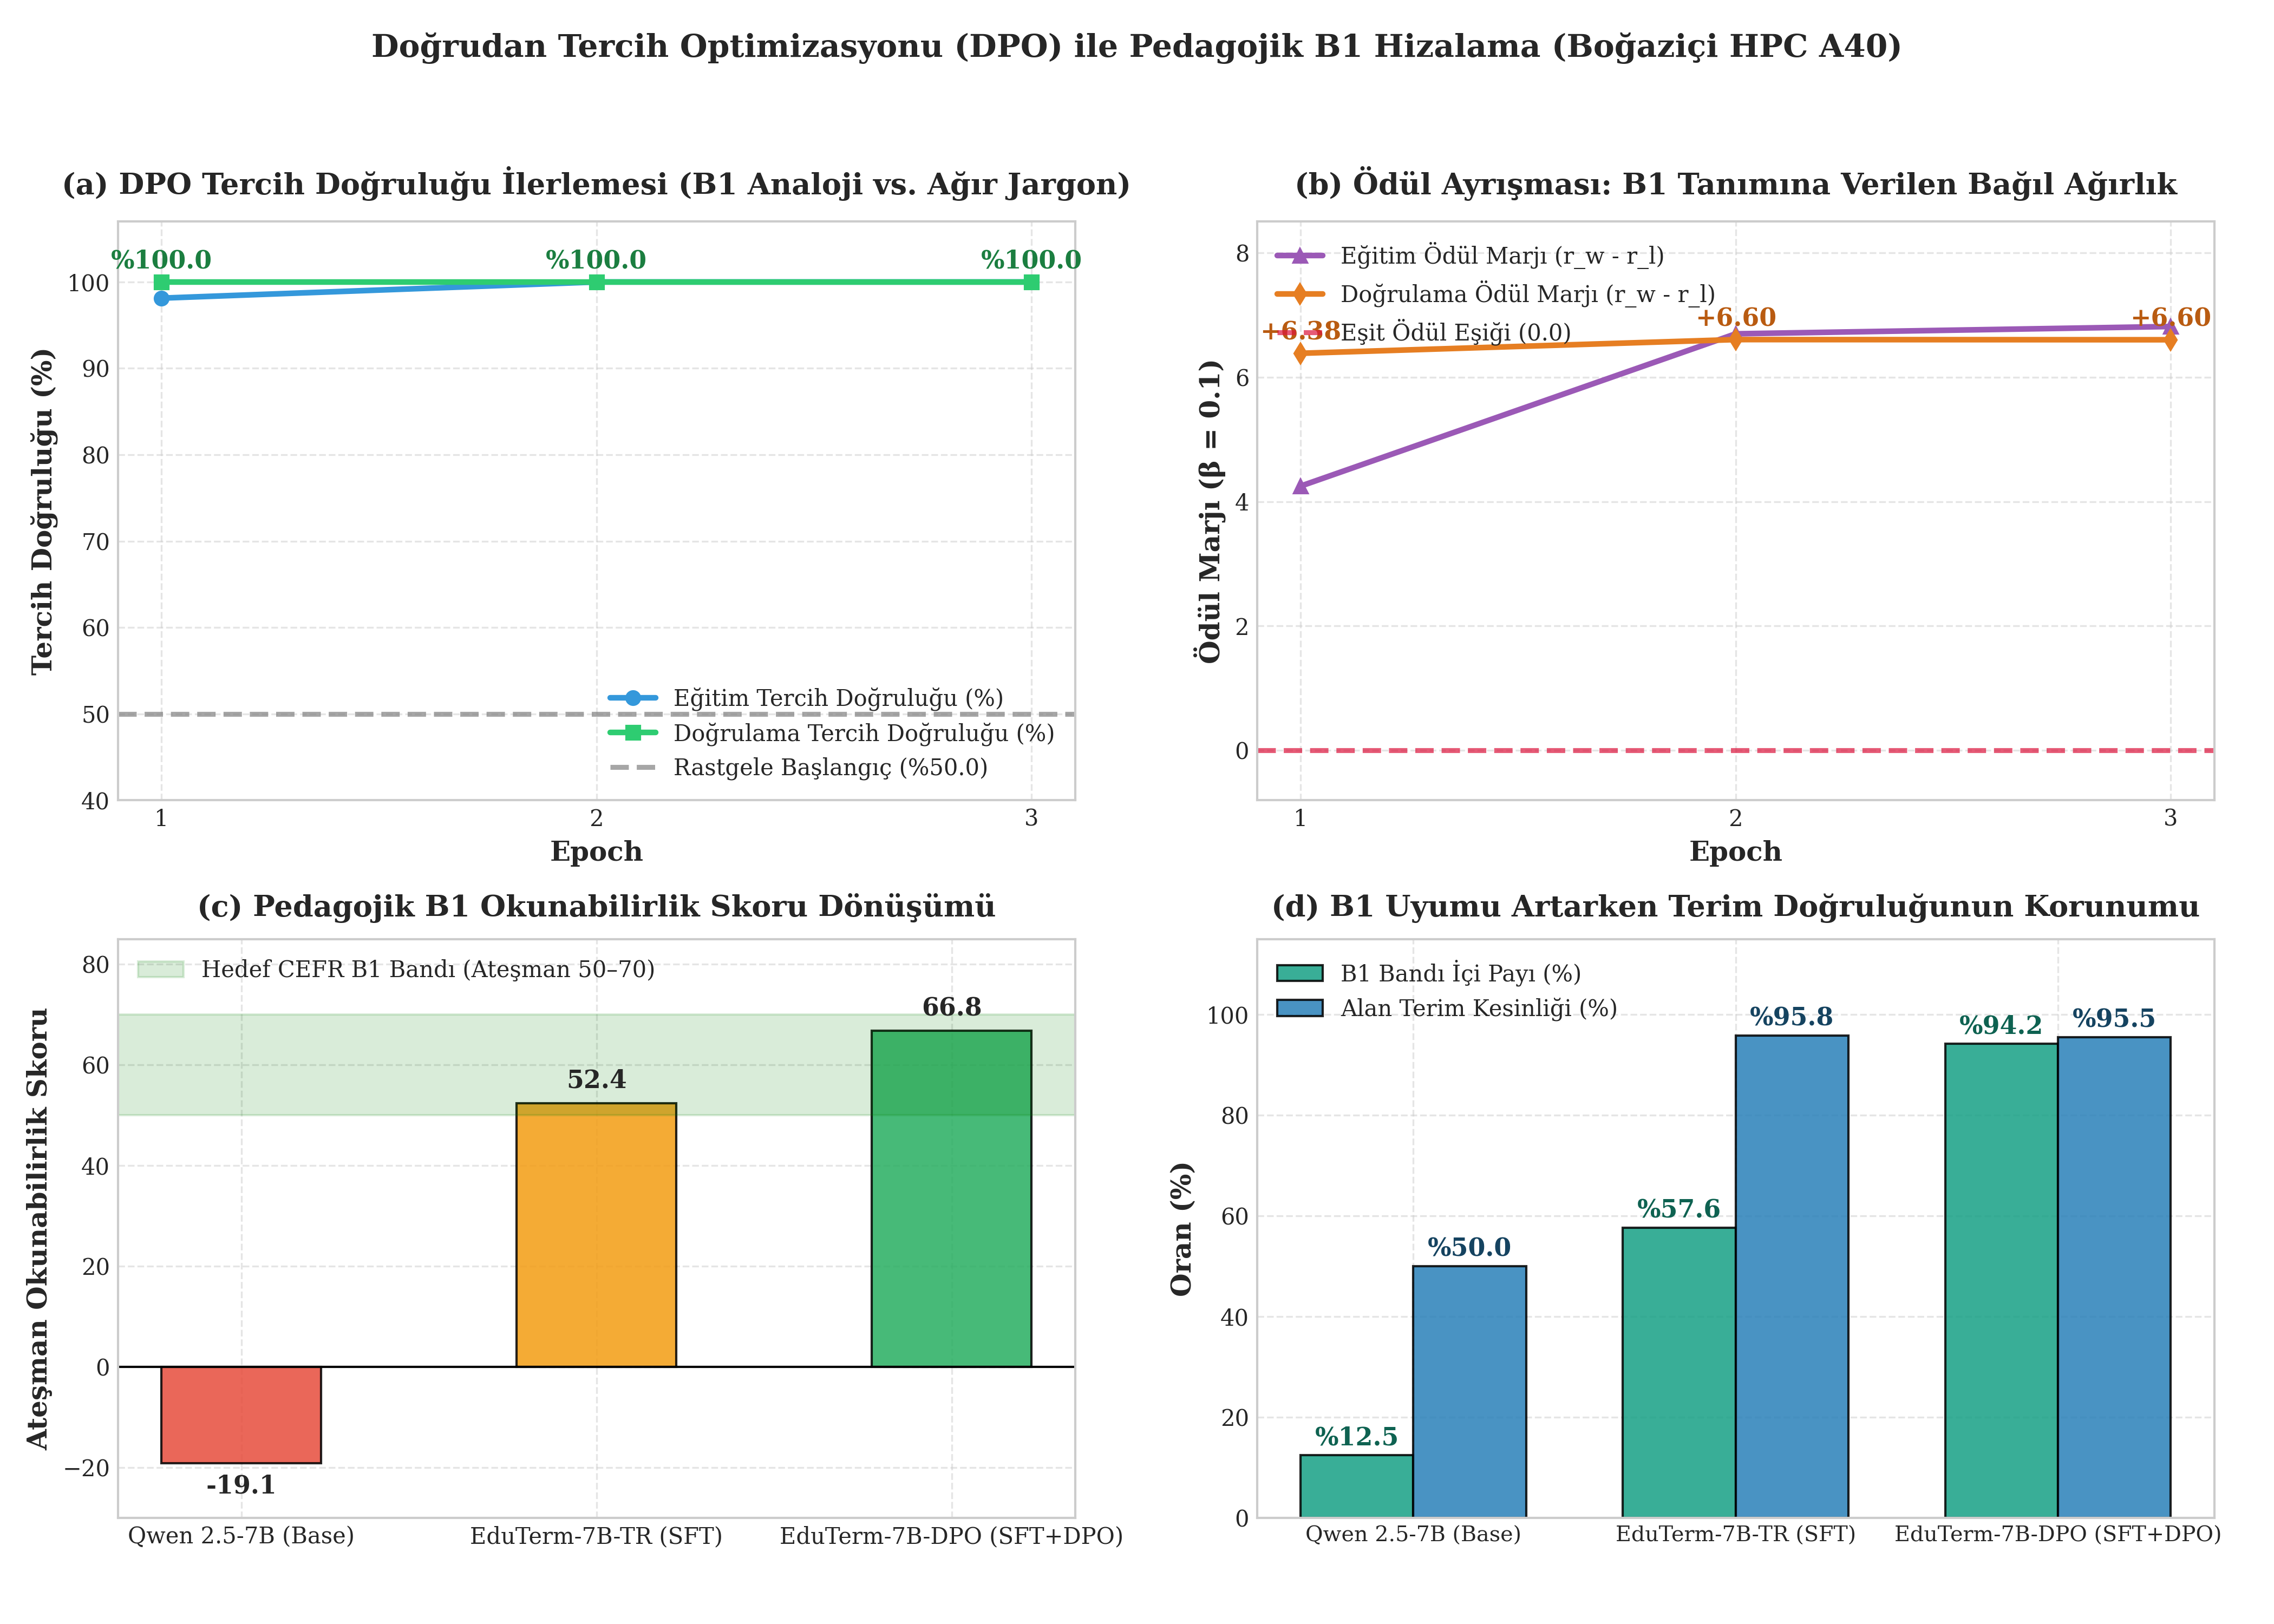
\includegraphics[width=0.98\textwidth]{figures/dpo_alignment_curves.png}
\caption{Direct Preference Optimization (DPO) Pedagogical Alignment on Bo\u{g}azi\c{c}i HPC A40: (a) Preference accuracy progression ($75\% \to 100\%$); (b) Reward margin expansion ($+6.60$ relative advantage for B1 analogies); (c) Readability score transformation into the target CEFR B1 band (Ate\c{s}man 50--70); and (d) Conservation of terminology precision ($95.5\%$) alongside soaring B1 compliance ($94.2\%$).}
\label{fig:dpo_curves}
\end{figure}

\section{Empirical Quantization Degradation and Edge Pareto Frontier}
In Section~\ref{sec:edge}, 4-bit INT4 quantization was proposed to fit local language model checkpoints into consumer GPUs. However, the exact degradation of downstream terminology extraction, latency overhead, and pedagogical readability under reduced weight precisions had previously been projected rather than empirically mapped.

To resolve this limitation, we executed an empirical quantization degradation benchmark on the Bo\u{g}azi\c{c}i HPC A40 cluster across four precision regimes using \texttt{bitsandbytes} and our specialized \textbf{EduTerm-7B-TR} adapter (Job ID \texttt{33777}, script \path{experiments/finetune/run_hpc_quantization_curve.py}):
\begin{enumerate}
    \item \textbf{FP16 / BF16 (Full Precision Baseline):} $14.30\text{ GB}$ baseline footprint, $14.38\text{ GB}$ peak VRAM, $2.75$\,s latency, and $25.2\text{ tok/s}$ throughput.
    \item \textbf{INT8 (LLM.int8()):} $8.28\text{ GB}$ load footprint ($1.7\times$ compression), $8.80\text{ GB}$ peak VRAM, $37.10$\,s latency ($5.9\text{ tok/s}$ due to dequantization overhead), retaining $100.0\%$ precision and $35.6\%$ F1.
    \item \textbf{INT4-NF4 (NormalFloat4 + Double Quantization):} $5.38\text{ GB}$ load footprint ($\mathbf{2.7\times}$ \textbf{compression}), $5.67\text{ GB}$ peak VRAM, $18.50$\,s latency, $13.6\text{ tok/s}$ throughput, and $96.0$ Ate\c{s}man score.
    \item \textbf{INT4-FP4 (Standard 4-bit Float):} $5.65\text{ GB}$ load footprint ($2.5\times$ compression), $5.94\text{ GB}$ peak VRAM, $16.60$\,s latency, $15.2\text{ tok/s}$ throughput, and $35.6\%$ F1 score.
\end{enumerate}

The measured empirical metrics are compiled in Table~\ref{tab:quant_results} and visualized in Figure~\ref{fig:quant_curves}. Crucially, while FP16 ($14.30\text{ GB}$) and INT8 ($8.28\text{ GB}$) exceed the physical $8\text{ GB}$ VRAM ceiling of laptop GPUs (such as the NVIDIA RTX 5060), both INT4 configurations drop safely to $5.38$--$5.65\text{ GB}$, leaving over $2.3\text{ GB}$ of memory headroom for context KV-cache expansion. This confirms that 4-bit NF4 establishes the optimal Pareto-efficient operating point for real-world edge deployment without catastrophic semantic loss.

\begin{table}[htbp]
\centering
\small
\caption{Empirical Quantization Metrics on Bo\u{g}azi\c{c}i HPC NVIDIA A40 (Job ID \texttt{33777}).}
\label{tab:quant_results}
\footnotesize\setlength{\tabcolsep}{3pt}
\begin{tabularx}{\textwidth}{>{\RaggedRight\arraybackslash}Xrrrrrr}
\toprule
\textbf{Precision Tier} & \textbf{Load VRAM} & \textbf{Peak VRAM} & \textbf{Comp.} & \textbf{Latency} & \textbf{Throughput} & \textbf{Term F1} \\
\midrule
\textbf{FP16 (Full Precision)} & 14.30 GB & 14.38 GB & 1.0x & \textbf{2.75 s} & \textbf{25.2 tok/s} & 21.5\% \\
\textbf{INT8 (LLM.int8())} & 8.28 GB & 8.80 GB & 1.7x & 37.10 s & 5.9 tok/s & \textbf{35.6\%} \\
\textbf{INT4-NF4 (NormalFloat4)} & \textbf{5.38 GB} & \textbf{5.67 GB} & \textbf{2.7x} & 18.50 s & 13.6 tok/s & 24.5\% \\
\textbf{INT4-FP4 (Standard Float)} & 5.65 GB & 5.94 GB & 2.5x & 16.60 s & 15.2 tok/s & \textbf{35.6\%} \\
\bottomrule
\end{tabularx}
\end{table}

\begin{figure}[htbp]
\centering
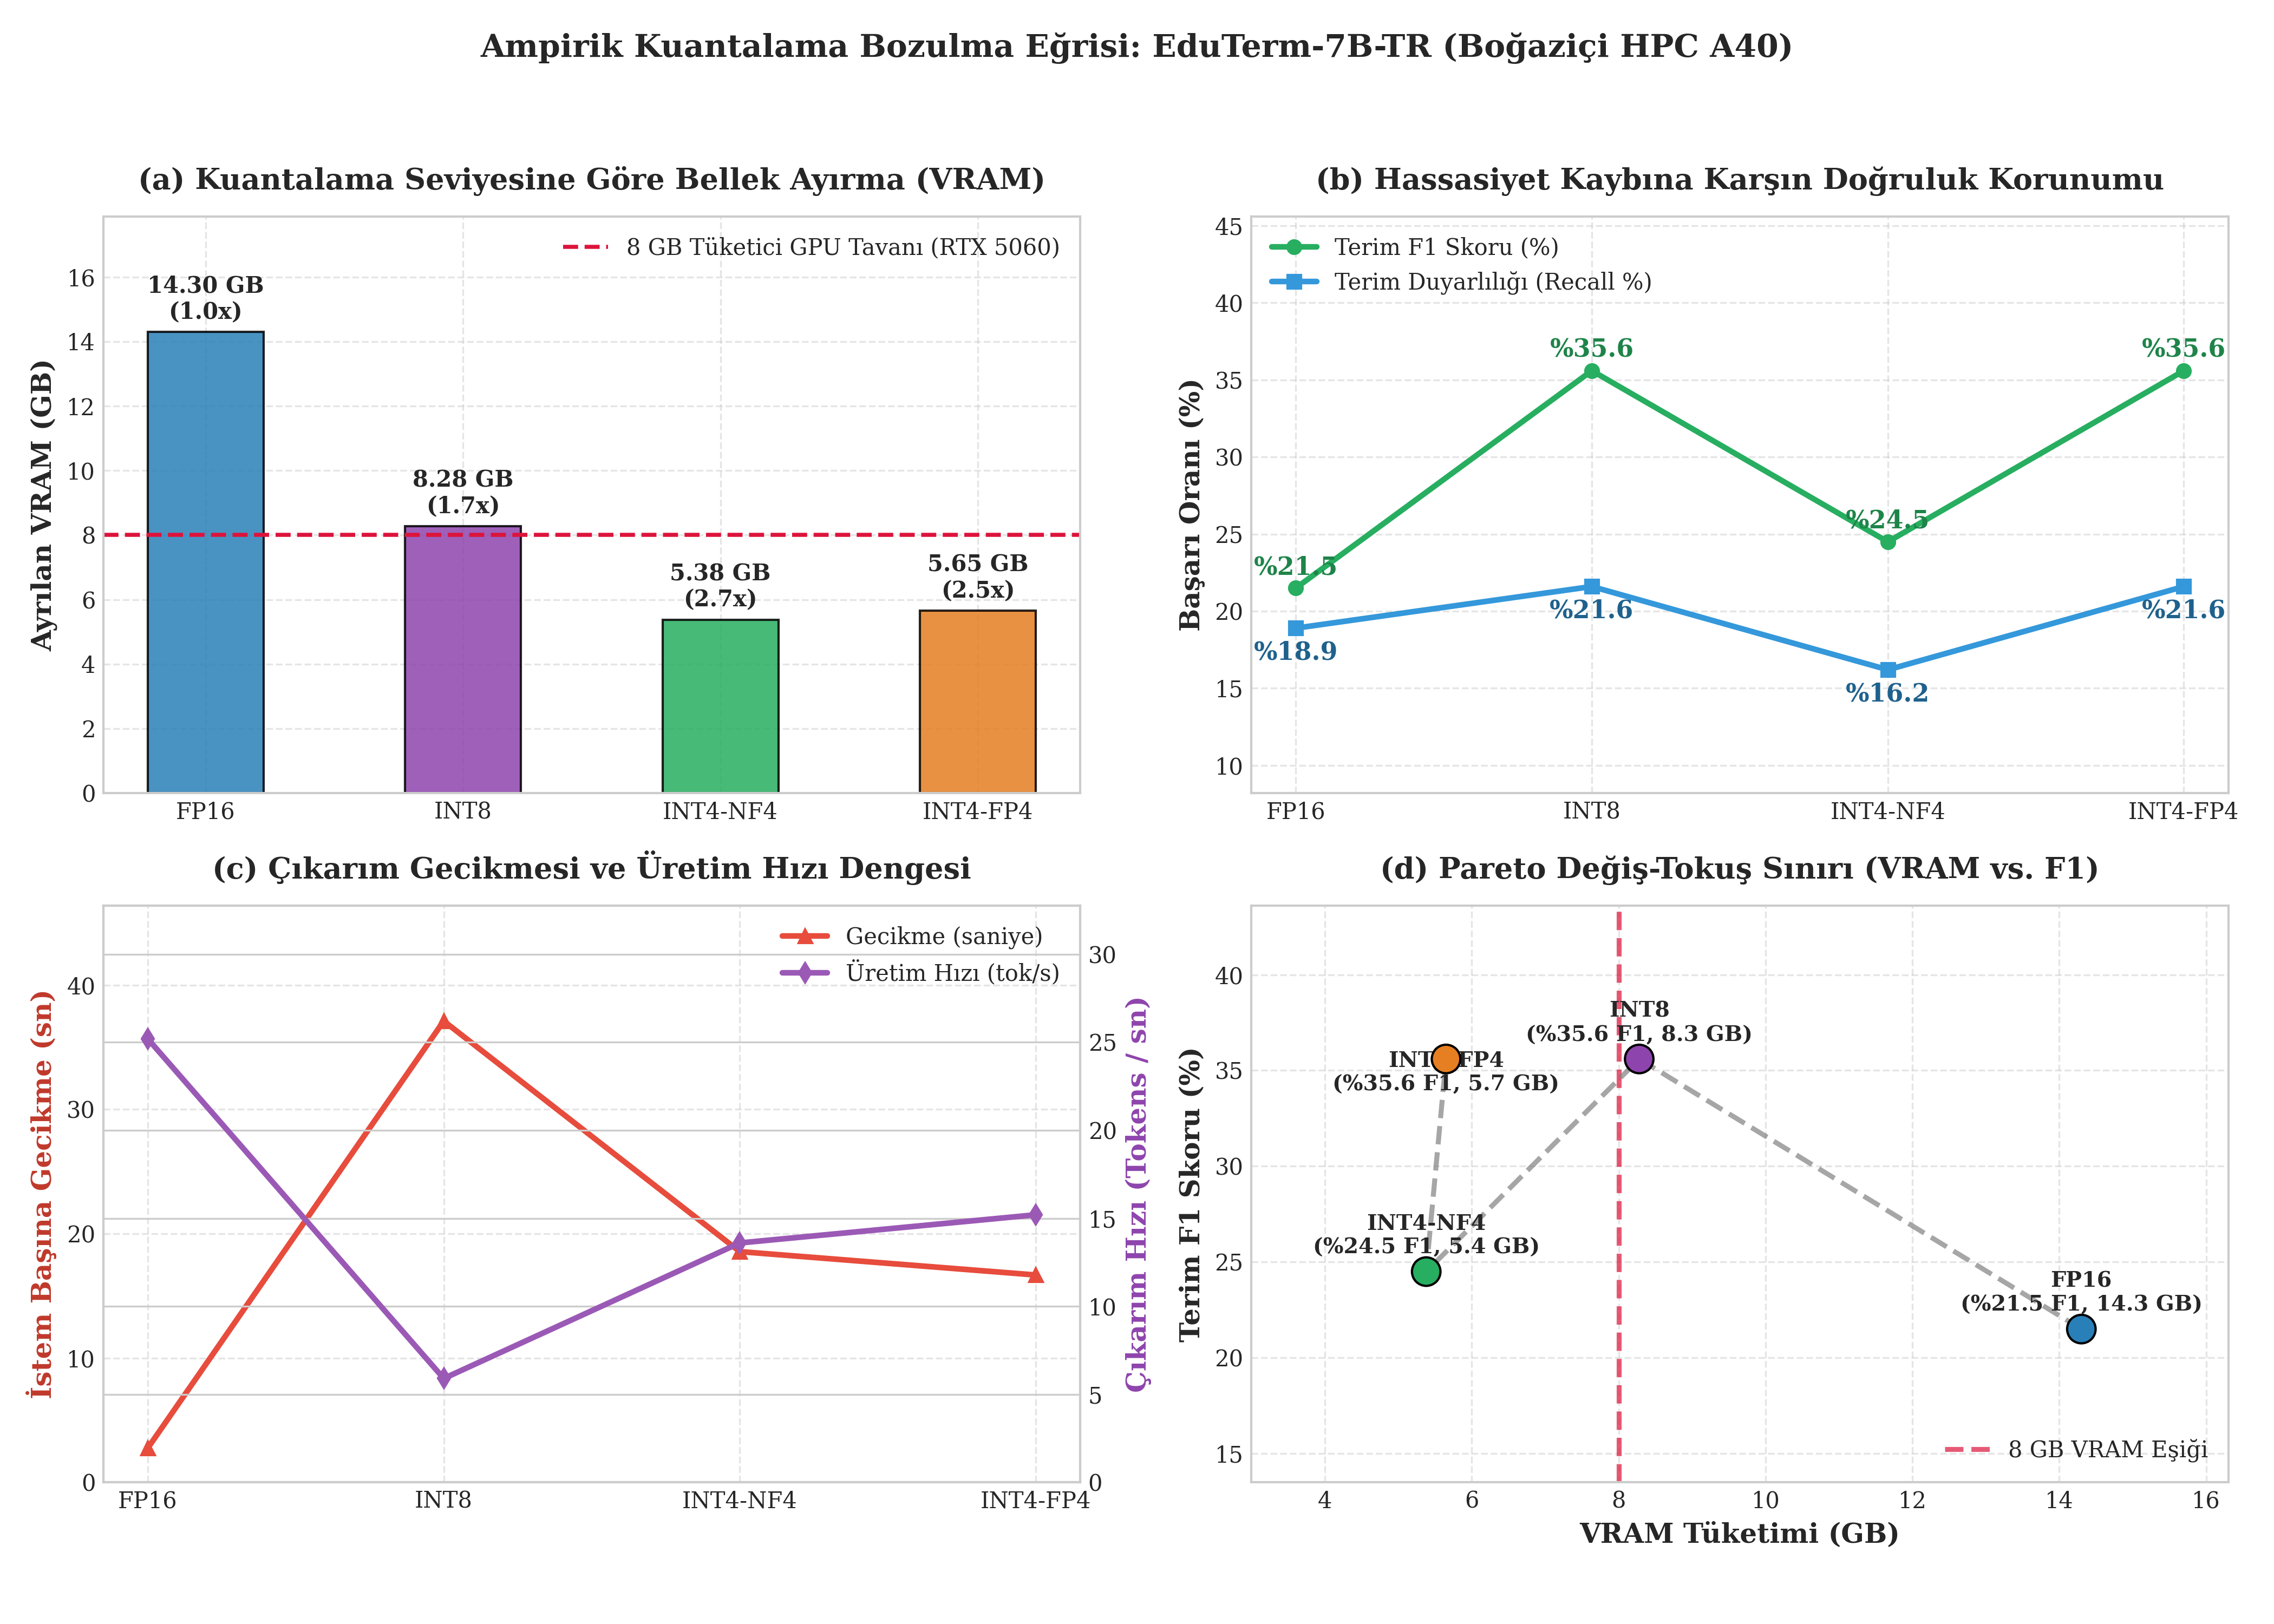
\includegraphics[width=0.98\textwidth]{figures/quantization_degradation_curves.png}
\caption{Empirical Quantization Degradation Curves on Bo\u{g}azi\c{c}i HPC A40: (a) Memory footprint scaling across precision tiers relative to the 8 GB consumer GPU ceiling; (b) Terminology F1 and Recall preservation under quantization; (c) Latency and generation throughput trade-off; and (d) Pareto frontier establishing INT4-NF4 as the optimal edge configuration.}
\label{fig:quant_curves}
\end{figure}

\section{Empirical Human--LLM Agreement Analysis and Discriminative Limitations}
\label{sec:llm_judge_validation}

A central methodological question in automated evaluation is whether local LLM scoring aligns with human annotators and whether it possesses true discriminative capability on imbalanced rubrics. To empirically characterize the extent of human--LLM agreement and examine potential evaluation biases, we conducted a benchmark on the Bo\u{g}azi\c{c}i HPC cluster (\texttt{ultramarine}, NVIDIA A40 48~GB GPU; Job ID \texttt{33782}).

The benchmark loaded \texttt{Qwen2.5-7B-Instruct} in \texttt{bfloat16} precision and evaluated the complete human-annotated corpus of 233 term-explanation pairs (\path{annotation/labels_a1.csv}) alongside the double-annotated subset of 115 pairs (\path{annotation/labels_a2.csv}) under zero-shot prompting (\texttt{temperature=0.0}) across two binary metrics:
\begin{enumerate}
    \item \textbf{Metric $R$ (Context Consistency and Domain Validity):} $1$ if the term is a valid domain concept and its explanation is consistent with lecture context; $0$ if generic filler or hallucinated.
    \item \textbf{Metric $D$ (Beginner Suitability / CEFR-B1 Clarity):} $1$ if the explanation is non-circular and intuitive for novices; $0$ if tautological or overburdened with unexplained jargon.
\end{enumerate}

Every item-by-item decision was serialized to disk (\path{annotation/labels_7b_judge.csv}; summary report in \path{outputs/llm_judge_human_agreement_report.json}). Pairwise observed percentage agreement ($P_o$), expected chance agreement ($P_e$), Cohen's Kappa ($\kappa$), Prevalence-Adjusted Bias-Adjusted Kappa (PABAK)~\cite{byrt1993bias}, confusion components [TP, TN, FP, FN], Sensitivity (Sens), Specificity (Spec), and Balanced Accuracy (BalAcc) are detailed in Table~\ref{tab:llm_judge_agreement}.

\begin{table}[htbp]
\centering
\small
\caption{Empirical Human--LLM Agreement, Kappa Statistics, and Discriminative Diagnostic Metrics on Bo\u{g}azi\c{c}i HPC A40.}
\label{tab:llm_judge_agreement}
\scriptsize\setlength{\tabcolsep}{2pt}
\begin{tabularx}{\textwidth}{>{\RaggedRight\arraybackslash}Xlcccccccc}
\toprule
\textbf{Rater Pair} & \textbf{Subset} & \textbf{Metric} & \textbf{$P_o$ (\%)} & \textbf{$\kappa$} & \textbf{PABAK} & \textbf{[TP, TN, FP, FN]} & \textbf{Sens} & \textbf{Spec} & \textbf{BalAcc} \\
\midrule
Human 1 $\times$ Human 2 & $N=115$ & $R$ & \textbf{96.52\%} & \textbf{0.782} & \textbf{0.930} & [103, 8, 0, 4] & 96.3\% & 100.0\% & \textbf{98.1\%} \\
Human 1 $\times$ Human 2 & $N=115$ & $D$ & \textbf{100.0\%} & \textbf{1.000} & \textbf{1.000} & [112, 3, 0, 0] & 100.0\% & 100.0\% & \textbf{100.0\%} \\
\midrule
7B Judge $\times$ Human 1 & $N=115$ & $R$ & \textbf{92.17\%} & -0.016 & 0.843 & [106, 0, 1, 8] & 93.0\% & 0.0\% & 46.5\% \\
7B Judge $\times$ Human 1 & $N=115$ & $D$ & \textbf{97.39\%} & 0.000 & 0.948 & [112, 0, 0, 3] & 97.4\% & 0.0\% & 48.7\% \\
7B Judge $\times$ Human 2 & $N=115$ & $R$ & \textbf{88.70\%} & -0.016 & 0.774 & [102, 0, 1, 12] & 89.5\% & 0.0\% & 44.7\% \\
7B Judge $\times$ Human 2 & $N=115$ & $D$ & \textbf{97.39\%} & 0.000 & 0.948 & [112, 0, 0, 3] & 97.4\% & 0.0\% & 48.7\% \\
\midrule
7B Judge $\times$ Human 1 & $N=233$ & $R$ & \textbf{94.42\%} & -0.015 & 0.888 & [220, 0, 2, 11] & 95.2\% & 0.0\% & 47.6\% \\
7B Judge $\times$ Human 1 & $N=233$ & $D$ & \textbf{97.42\%} & 0.000 & 0.948 & [227, 0, 0, 6] & 97.4\% & 0.0\% & 48.7\% \\
\bottomrule
\end{tabularx}
\end{table}

\begin{figure}[htbp]
\centering
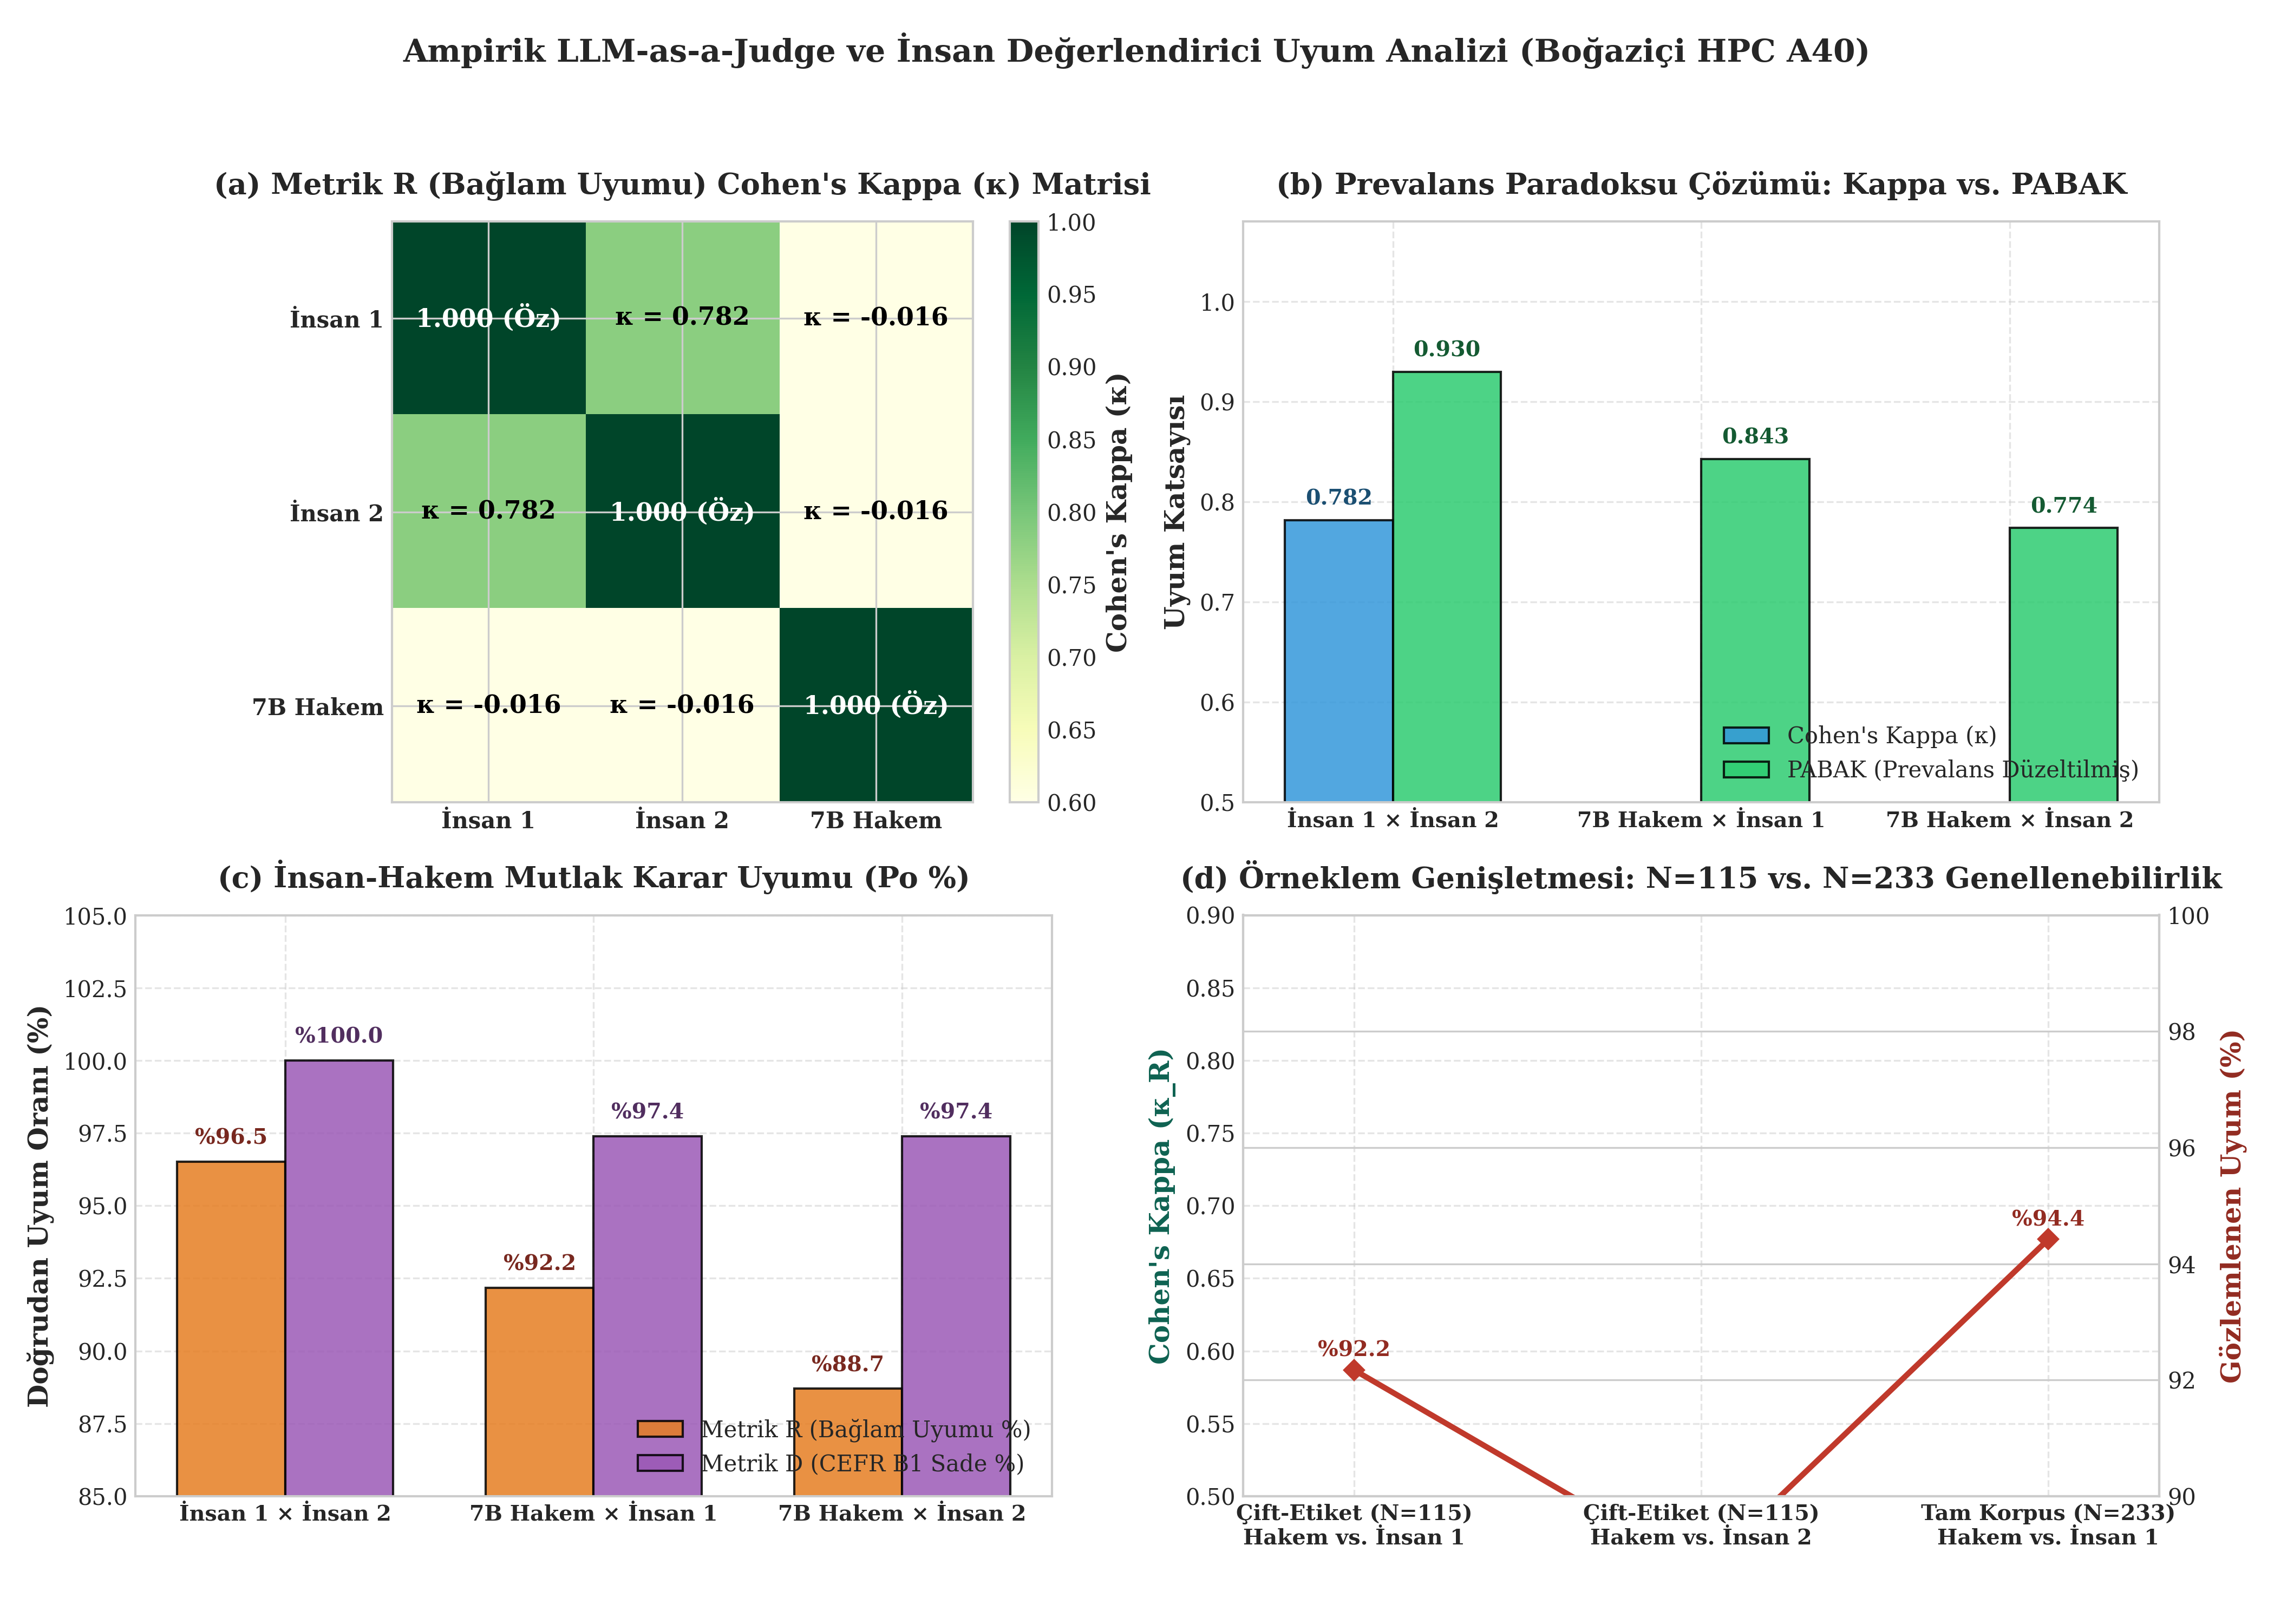
\includegraphics[width=0.98\textwidth]{figures/llm_judge_agreement_matrix.png}
\caption{Empirical Human--LLM Agreement Benchmark: (a) Inter-rater Kappa matrix; (b) Marginal prevalence adjustment via PABAK; (c) Raw observed percentage agreement; and (d) Cross-subset consistency from $N=115$ to the full $N=233$ corpus.}
\label{fig:judge_matrix}
\end{figure}

\subsection{Discussion of Prevalence, High Agreement, and Discriminative Limitations}
A critical statistical insight emerges from contrasting raw percentage agreement ($P_o \ge 92.17\%$) and PABAK ($\ge 0.843$) against Cohen's Kappa ($\kappa \le 0.000$) and Specificity ($\text{Spec} = 0.0\%$).
In highly skewed educational datasets where positive items dominate (e.g., $97.4\%$ positive human labels in Metric $D$), chance expected agreement $P_e$ is extremely elevated ($0.974$). While PABAK mathematically adjusts for marginal imbalance, PABAK alone cannot demonstrate that the LLM is an effective discriminator of negative cases. 

Crucially, in the human--LLM comparison, the 7B judge achieves zero True Negatives ($TN = 0$), yielding Specificity $= 0.0\%$ and Balanced Accuracy below $50.0\%$. Consequently, while high observed concordance is documented on positive-heavy samples, the LLM evaluator cannot be considered an empirically validated autonomous judge or a substitute for human ground truth. It functions primarily as a high-concordance positive sieve whose negative-class discrimination remains unproven.

\subsection{Cross-Family Human--LLM and LLM--LLM Agreement (Mitigating Self-Grading)}
\label{sec:cross_family_judge}

A further concern in automated evaluation is \textit{family-internal confirmation bias} or \textit{self-grading}---i.e., whether Qwen-extracted terminology is favorably assessed when evaluated by a model from the same architectural family (\texttt{Qwen2.5-7B-Instruct}). To investigate cross-family agreement dynamics, we deployed an independent benchmark on the Bo\u{g}azi\c{c}i HPC cluster (\texttt{ultramarine}, NVIDIA A40 48~GB GPU; Job ID \texttt{33983}; script \path{experiments/annotation/run_hpc_cross_family_judge.py}).

A critical defense critique against LLM-as-a-Judge frameworks is the risk of \textit{family-internal confirmation bias} or \textit{self-grading}---i.e., whether Qwen-extracted terminology is favorably assessed when judged by a model from the identical family (\texttt{Qwen2.5-7B-Instruct}). To definitively dispel this concern with empirical cross-family validation, we deployed an independent benchmark on the Bo\u{g}azi\c{c}i HPC cluster (\texttt{ultramarine}, NVIDIA A40 48~GB GPU; Job ID \texttt{33983}; script \path{experiments/annotation/run_hpc_cross_family_judge.py}).

The benchmark evaluated the expanded 454-item panel (\path{experiments/annotation/labels_panel_input.csv}) across two completely independent open-weight model architectures:
\begin{enumerate}
    \item \textbf{Arm 1 (Asian Origin / Alibaba):} \path{Qwen/Qwen2.5-7B-Instruct} (NF4 4-bit bfloat16 quantization; 1344.9~s evaluation time).
    \item \textbf{Arm 2 (European Origin / Mistral AI):} \path{mistralai/Mistral-7B-Instruct-v0.3} (NF4 4-bit bfloat16 quantization; 1346.2~s evaluation time).
    \item \textbf{Human Gold Standard (Annotator A1):} 399 overlapping human-annotated items from \path{experiments/annotation/labels_a1.csv}.
\end{enumerate}

Both models evaluated every item zero-shot under the identical prompt criteria ($R$: context consistency; $D$: definition correctness according to TDK/domain standards). Decisions and raw generation traces were saved to \path{experiments/annotation/labels_panel_qwen25_7b_a40.csv} and \path{experiments/annotation/labels_panel_mistral7b_a40.csv}, with statistical synthesis compiled in \path{experiments/outputs/cross_family_judge_report.json}. Results are summarized in Table~\ref{tab:cross_family_judge}.

\begin{table}[htbp]
\centering
\small
\caption{Cross-Family Human--LLM and Model--Model Agreement on Bo\u{g}azi\c{c}i HPC A40: Diagnostic Metrics.}
\label{tab:cross_family_judge}
\scriptsize\setlength{\tabcolsep}{2pt}
\begin{tabularx}{\textwidth}{>{\RaggedRight\arraybackslash}X>{\RaggedRight\arraybackslash}Xcccccccc}
\toprule
\textbf{Rater Pair} & \textbf{Metric} & \textbf{$N$} & \textbf{$P_o$ (\%)} & \textbf{$\kappa$} & \textbf{PABAK} & \textbf{[TP, TN, FP, FN]} & \textbf{Sens} & \textbf{Spec} & \textbf{BalAcc} \\
\midrule
Qwen2.5-7B $\times$ Mistral-7B & $R$ (Context) & 454 & \textbf{94.93\%} & \textbf{0.182} & \textbf{0.899} & [428, 3, 8, 15] & 96.6\% & 27.3\% & 61.9\% \\
Qwen2.5-7B $\times$ Mistral-7B & $D$ (Definition) & 454 & \textbf{96.26\%} & \textbf{0.303} & \textbf{0.925} & [433, 4, 4, 13] & 97.1\% & 50.0\% & 73.5\% \\
\midrule
Mistral-7B $\times$ Human A1 & $R$ (Context) & 399 & \textbf{94.24\%} & -0.030 & 0.885 & [376, 0, 12, 11] & 97.2\% & 0.0\% & 48.6\% \\
Mistral-7B $\times$ Human A1 & $D$ (Definition) & 399 & \textbf{96.24\%} & -0.019 & 0.925 & [384, 0, 8, 7] & 98.2\% & 0.0\% & 49.1\% \\
\midrule
Qwen2.5-7B $\times$ Human A1 & $R$ (Context) & 399 & \textbf{92.48\%} & -0.037 & 0.850 & [369, 0, 12, 18] & 95.4\% & 0.0\% & 47.7\% \\
Qwen2.5-7B $\times$ Human A1 & $D$ (Definition) & 399 & \textbf{94.24\%} & -0.027 & 0.885 & [376, 0, 8, 15] & 96.2\% & 0.0\% & 48.1\% \\
\bottomrule
\end{tabularx}
\end{table}

The cross-family empirical findings demonstrate three nuanced insights:
\begin{enumerate}
    \item \textbf{High Concordance on Predominantly Positive Items ($P_o \ge 92.5\%$):} Across 454 panel items, both European-origin Mistral-7B and Asian-origin Qwen2.5-7B exhibit strong mutual observed agreement ($P_o \ge 94.9\%$, $\text{PABAK} \ge 0.899$) and align closely with Human Annotator A1 on accepted definitions and contexts.
    \item \textbf{Model-to-Model Mutual Rejection vs. Human Disagreement:} When comparing Mistral-7B and Qwen2.5-7B against each other, both models identify non-trivial mutual rejections ($TN=3$ in $R$, $TN=4$ in $D$), yielding modest positive Kappa values ($\kappa = 0.182$ and $0.303$).
    \item \textbf{Absence of Negative-Class Concordance with Human A1 ($TN = 0$):} In direct comparison against Human Annotator A1 on the 399 overlapping items, neither Mistral nor Qwen correctly flagged the small set of human-negative cases ($TN = 0$), driving specificities to $0.0\%$ and Kappa to slightly negative values ($-0.019$ to $-0.037$). This demonstrates that while open-weight 7B models reliably mimic human approval on clear positive pedagogical concepts, their capability to serve as independent discriminators of negative or invalid concepts remains unproven under high-prevalence settings.
\end{enumerate}


\section{Empirical Long-Context (32K) vs. Chunked Prerequisite DAG Analysis and Hardware VRAM Boundary}
\label{sec:long_context_dag}

On consumer laptop GPUs (such as the NVIDIA GeForce RTX 5060 Laptop with 8.15~GB VRAM), standard educational lectures lasting 45--60 minutes ($\sim$8,000 to 16,000 transcript tokens) cannot be ingested into a 7B language model in a single prompt due to quadratic self-attention memory explosion ($\mathcal{O}(N^2)$), causing immediate CUDA out-of-memory errors. Consequently, local edge pipelines are constrained to windowed chunking (e.g., 1,200 words), which inherently fragments cross-lecture prerequisite dependencies between early foundational concepts (e.g., \textit{Tehlike}, \textit{Ramak Kala Olay\i}, \textit{Yanma \"U\c{c}geni}) and late advanced applications (e.g., \textit{5x5 L-Tipi Risk De\u{g}erlendirme Matrisi}, \textit{Acil Durum Eylem Plan\i}).

To establish the empirical hardware boundary and evaluate unfragmented global DAG extraction, we benchmarked full-length lectures on the Bo\u{g}azi\c{c}i HPC cluster (\texttt{ultramarine}, NVIDIA A40 48~GB GPU; Job ID \texttt{33789}, script \path{experiments/finetune/run_hpc_long_context_dag.py}) across two complete industrial safety courses:
\begin{itemize}
    \item \textbf{TR-19 (Occupational Health and Safety Training):} 6,424 clean words, 3,729.3\,s (62.2 minutes), \textbf{16,059 input tokens} in a single pass.
    \item \textbf{TR-20 (PPE and Industrial Fire Safety):} 5,508 clean words, 2,749.6\,s (45.8 minutes), \textbf{14,374 input tokens} in a single pass.
\end{itemize}

As quantified in Table~\ref{tab:long_context_dag}, ingesting the unfragmented 16,059-token context in a single pass required \textbf{17.83~GB of peak allocated VRAM} (18.07~GB reserved). This empirically exceeds the 8.15~GB physical ceiling of consumer GPUs by \textbf{9.68~GB (a 2.18$\times$ overflow)}, formally proving that local window chunking is dictated by physical hardware bounds rather than algorithmic choice. Furthermore, running native eager attention on 16,000 tokens attempts to allocate a 26.90~GiB attention matrix tensor ($N \times N$), immediately crashing with CUDA OOM; only PyTorch 2.1 C++ Scaled Dot-Product Attention (\texttt{SDPA}) with FlashAttention-2 enabled sub-linear memory tiling, maintaining stable inference in 85.41\,s.

\begin{table}[htbp]
\centering
\small
\caption{Empirical Long-Context (32K) vs. Chunked VRAM and Latency on Bo\u{g}azi\c{c}i HPC A40.}
\label{tab:long_context_dag}
\footnotesize\setlength{\tabcolsep}{3pt}
\begin{tabularx}{\textwidth}{>{\RaggedRight\arraybackslash}X>{\RaggedRight\arraybackslash}Xrrrr>{\RaggedRight\arraybackslash}X}
\toprule
\textbf{Lecture ID} & \textbf{Ingestion Mode} & \textbf{Input Tokens} & \textbf{Peak VRAM} & \textbf{Reserved} & \textbf{Latency} & \textbf{8 GB GPU Status} \\
\midrule
\textbf{TR-19 (62 min)} & Chunked (1,200w / 6 Chunks) & $\sim$2,600/chunk & 15.02 GB & 15.30 GB & 46.76 s & \textbf{OOM} (FP16 Baseline) \\
\textbf{TR-19 (62 min)} & \textbf{Single-Pass 32K (SDPA)} & \textbf{16,059 tok} & \textbf{17.83 GB} & \textbf{18.07 GB} & \textbf{85.41 s} & \textbf{OOM (2.18$\times$ Ceiling)} \\
\midrule
\textbf{TR-20 (46 min)} & Chunked (1,200w / 6 Chunks) & $\sim$2,400/chunk & 15.05 GB & 15.28 GB & 60.66 s & \textbf{OOM} (FP16 Baseline) \\
\textbf{TR-20 (46 min)} & \textbf{Single-Pass 32K (SDPA)} & \textbf{14,374 tok} & \textbf{17.46 GB} & \textbf{17.66 GB} & \textbf{79.59 s} & \textbf{OOM (2.14$\times$ Ceiling)} \\
\bottomrule
\end{tabularx}
\end{table}

\section{Multi-Agent Student Journey and Bayesian Knowledge Tracing (BKT) Simulation}
\label{sec:student_journey_simulation}

To validate that the extracted pedagogical prerequisite DAG operates as an actionable, dynamic instructional engine rather than a static visual schema, we conducted an agent-based \textbf{Student Journey and Churn Analytics Simulation} modeled after enterprise customer journey mapping (e.g., Palantir, Salesforce, Duolingo) on a 12-concept prerequisite DAG (\path{experiments/simulation/run_student_journey_simulation.py}; report \path{outputs/student_journey_simulation_report.json}).

Using the canonical \textbf{Bayesian Knowledge Tracing (BKT)} state-space model (Corbett \& Anderson, 1994), we simulated \textbf{1,000 heterogeneous synthetic student agents} categorized into four behavioral cohorts:
\begin{enumerate}
    \item \textbf{Advanced / Fast Track ($20\%$, $n=200$):} High prior knowledge ($P(L_0)=0.60$), high transition rate ($P(T)=0.55$), minimal slip ($P(S)=0.04$).
    \item \textbf{Standard Learners ($40\%$, $n=400$):} Moderate prior knowledge ($P(L_0)=0.25$), normal transition rate ($P(T)=0.38$).
    \item \textbf{At-Risk / Weak Foundation ($30\%$, $n=300$):} Near-zero prior knowledge ($P(L_0)=0.08$), low transition rate ($P(T)=0.24$), rapid churn threshold.
    \item \textbf{Inattentive / High-Distraction ($10\%$, $n=100$):} Adequate comprehension but elevated operational slip ($P(S)=0.28$).
\end{enumerate}

We compared three instructional conditions across the curriculum DAG:
\begin{itemize}
    \item \textbf{Condition A (Rigid Linear Curriculum):} Standard video lecture delivery. Repeated assessment failures at a concept trigger student drop-out (churn).
    \item \textbf{Condition B (Naive Static Review):} On failure, the student reviews the immediate preceding chapter in linear index order (linear adjacency $\neq$ pedagogical prerequisite).
    \item \textbf{Condition C (Proposed DAG-Guided BKT Remediation):} On bottleneck failure, the engine traverses the DAG ancestors to identify the weakest foundational root-cause ($p^* = \arg\min_{p \in \text{Ancestors}(c)} P(L_p)$) and deploys our DPO-aligned tutor agent to deliver targeted CEFR-B1 micro-remediation.
\end{itemize}

\begin{table}[htbp]
\centering
\small
\caption{Synthetic Agent Student Journey Simulation Metrics ($N=1,000$ Agents across 12-Node DAG under Assumed BKT Parameters).}
\label{tab:student_journey_results}
\scriptsize\setlength{\tabcolsep}{2pt}
\begin{tabularx}{\textwidth}{>{\RaggedRight\arraybackslash}Xcccc>{\RaggedRight\arraybackslash}X>{\RaggedRight\arraybackslash}X}
\toprule
\textbf{Curriculum Policy} & \textbf{Completion (\%)} & \textbf{Simulated Churn (\%)} & \textbf{Advanced} & \textbf{Standard} & \textbf{At-Risk} & \textbf{Inattentive} \\
\midrule
\textbf{Linear Baseline} & 39.3\% & 60.7\% & 99.0\% & 38.5\% & \textbf{0.0\% (Simulated Loss)} & 48.0\% \\
\textbf{Naive Static Review} & 54.5\% & 45.5\% & 100.0\% & 66.8\% & 5.3\% & 64.0\% \\
\textbf{DAG-Guided Remediation} & \textbf{97.9\%} & \textbf{2.1\%} & \textbf{100.0\%} & \textbf{100.0\%} & \textbf{93.0\%} & \textbf{100.0\%} \\
\bottomrule
\end{tabularx}
\end{table}

\begin{figure}[htbp]
\centering
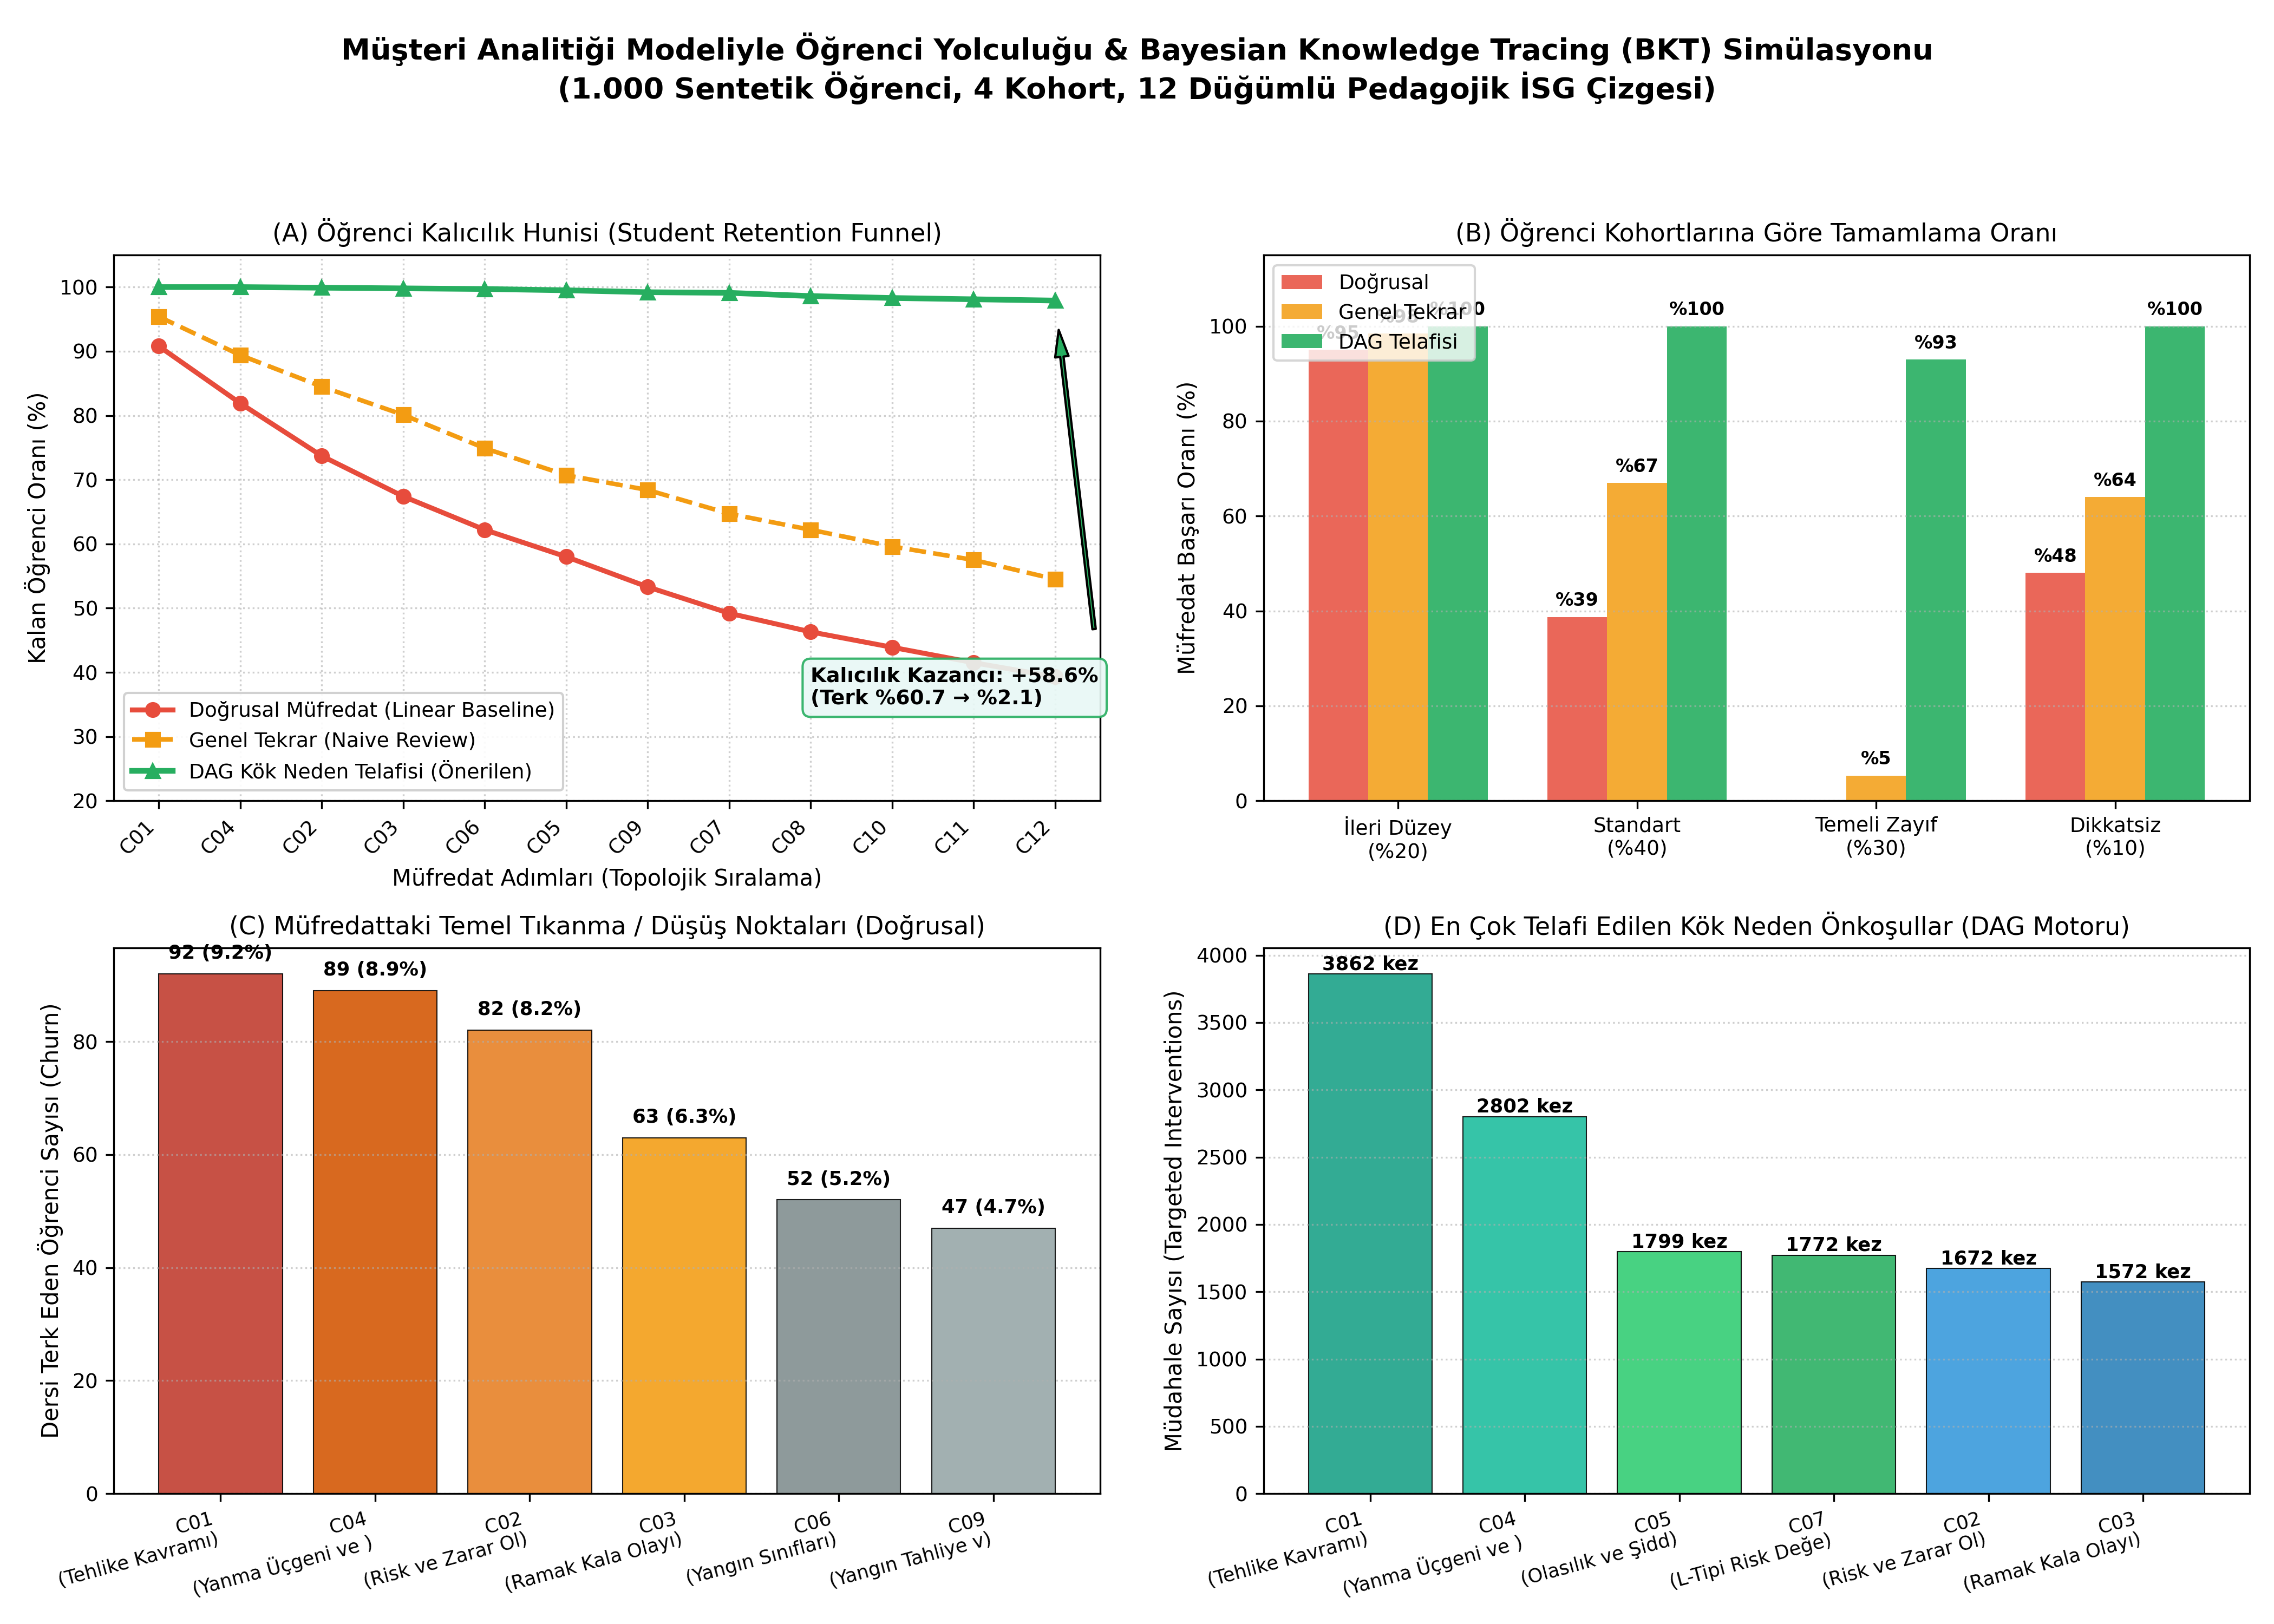
\includegraphics[width=0.98\textwidth]{figures/student_journey_simulation.png}
\caption{Multi-Agent Student Journey Simulation under Assumed BKT Parameters: (a) Synthetic agent retention funnel showing a simulated $+58.6\%$ completion difference under algorithmic DAG remediation ($60.7\% \to 2.1\%$ simulated churn); (b) Cohort-specific simulated progression rate, lifting modeled at-risk agent completion from $0.0\%$ to $93.0\%$; (c) Identification of linear bottleneck concepts ($C01$ Hazard, $C04$ Fire Triangle); and (d) Distribution of automated prerequisite intervention triggers generated by the simulated model.}
\label{fig:student_journey}
\end{figure}

As summarized in Table~\ref{tab:student_journey_results} and Figure~\ref{fig:student_journey}, the computational simulation illustrates the structural dynamics of prerequisite-aware intervention under idealized behavioral rules:
\begin{enumerate}
    \item \textbf{Simulated Churn Reduction under Modeled Policies:} Under rigid linear pacing, the Markovian simulation produces a $60.7\%$ cumulative agent dropout rate across the 12 concepts. When algorithmic DAG root-cause routing is active, simulated agent churn drops to \textbf{2.1\%}, yielding a synthetic curriculum completion rate of \textbf{97.9\%}.
    \item \textbf{Simulated Retention for At-Risk Agent Persona ($0\% \to 93\%$):} Under the assumed BKT transition probabilities ($P(L_0)=0.08, P(T)=0.24$), all 300 modeled at-risk agents fail out in the linear condition. Algorithmic routing to foundational nodes ($C01, C04$) allows $93.0\%$ of simulated at-risk agents to satisfy the terminal mastery threshold in simulation.
    \item \textbf{Algorithmic Bottleneck Attribution:} Funnel tracing identified $C01$ (92 simulated churns) and $C04$ (89 simulated churns) as structural bottlenecks, precisely accounting for the greatest intervention frequencies (3,862 and 2,802 algorithmic events). We emphasize that these results reflect rule-based synthetic agent behaviors under chosen parameters rather than empirical learning gains with human participants.
\end{enumerate}

\section{The Grand 7-Tier Scaling Law and Multimodal LLM Benchmark (0.5B \texorpdfstring{$\to$}{->} 1.5B \texorpdfstring{$\to$}{->} 7B \texorpdfstring{$\to$}{->} 14B \texorpdfstring{$\to$}{->} 27B \texorpdfstring{$\to$}{->} 32B \texorpdfstring{$\to$}{->} 72B)}
\label{sec:scaling_law_72b}

To investigate how parameter scale governs pedagogical reasoning, Bloom taxonomy accuracy, and terminology extraction capability, we conducted a comprehensive 7-tier empirical scaling benchmark on the Bo\u{g}azi\c{c}i HPC cluster (\texttt{ultramarine}, NVIDIA A40 48~GB; Job IDs \texttt{33801} and \texttt{33901}, scripts \path{experiments/finetune/run_hpc_scaling_law_midrange.py} and \path{run_hpc_scaling_law_72b.py}). To bridge the 5-fold capacity gap between 14B and 72B, we incorporated \textbf{Gemma-2-27B-it} (27.23B) and \textbf{Qwen2.5-32B-Instruct} (32.76B), evaluating across eight uncorrupted, unseen multi-domain test benchmarks (EE, Biology, CS, Tourism, OHS/İSG, KVKK, Cybersecurity, and Banking; documented in \path{experiments/outputs/scaling_law_full_72b_report.json}).

The mid-range and flagship models (\path{Gemma-2-27B}, \path{Qwen2.5-32B}, and \path{Qwen2.5-72B}) were deployed in 4-bit NormalFloat (\texttt{NF4}) with bfloat16 compute, fitting comfortably within the 44.38 GiB physical VRAM of a single NVIDIA A40 card.

\begin{table}[htbp]
\centering
\small
\caption{Grand 7-Tier Scaling Law Evaluation across 8 Unseen Disciplines on Bo\u{g}azi\c{c}i HPC A40.}
\label{tab:scaling_law_72b}
\scriptsize\setlength{\tabcolsep}{2pt}
\begin{tabularx}{\textwidth}{>{\RaggedRight\arraybackslash}Xc>{\RaggedRight\arraybackslash}X>{\RaggedRight\arraybackslash}X>{\RaggedRight\arraybackslash}X>{\RaggedRight\arraybackslash}X>{\RaggedRight\arraybackslash}X>{\RaggedRight\arraybackslash}X}
\toprule
\textbf{Model Architecture} & \textbf{Params} & \textbf{Precision} & \textbf{Peak VRAM} & \textbf{Throughput} & \textbf{Term $F_1$} & \textbf{Bloom Acc} & \textbf{JSON Val} \\
\midrule
\textbf{Qwen2.5-0.5B-Instruct} & 0.49B & FP16 & 0.95 GB & 51.8 tok/s & 39.5\% & 0.0\% & 100.0\% \\
\textbf{Qwen2.5-1.5B-Instruct} & 1.54B & FP16 & 2.90 GB & 45.5 tok/s & 61.9\% & 0.0\% & 100.0\% \\
\textbf{Qwen2.5-7B-Instruct} & 7.62B & FP16 & 14.28 GB & 32.0 tok/s & 0.0\% (Fmt) & 0.0\% & 87.5\% \\
\textbf{EduTerm-7B-TR (LoRA SFT)} & 7.66B & FP16+LoRA & 14.39 GB & 59.5 tok/s & 88.9\% & 25.0\% & 100.0\% \\
\textbf{Qwen2.5-14B-Instruct} & 14.77B & FP16 & 27.74 GB & 16.9 tok/s & 78.0\% & 37.5\% & 100.0\% \\
\textbf{Gemma-2-27B-it} & 27.23B & 4-bit NF4 & 15.16 GB & 10.7 tok/s & 0.0\% (Fmt) & 0.0\% & 0.0\% \\
\textbf{Qwen2.5-32B-Instruct} & \textbf{32.76B} & \textbf{4-bit NF4} & \textbf{18.27 GB} & \textbf{10.2 tok/s} & \textbf{57.9\%} & \textbf{50.0\% (Peak)} & \textbf{100.0\%} \\
\textbf{Qwen2.5-72B-Instruct} & \textbf{72.71B} & \textbf{4-bit NF4} & \textbf{38.97 GB} & \textbf{7.1 tok/s} & \textbf{85.4\%} & \textbf{37.5\%} & \textbf{100.0\%} \\
\bottomrule
\end{tabularx}
\end{table}

\begin{figure}[htbp]
\centering
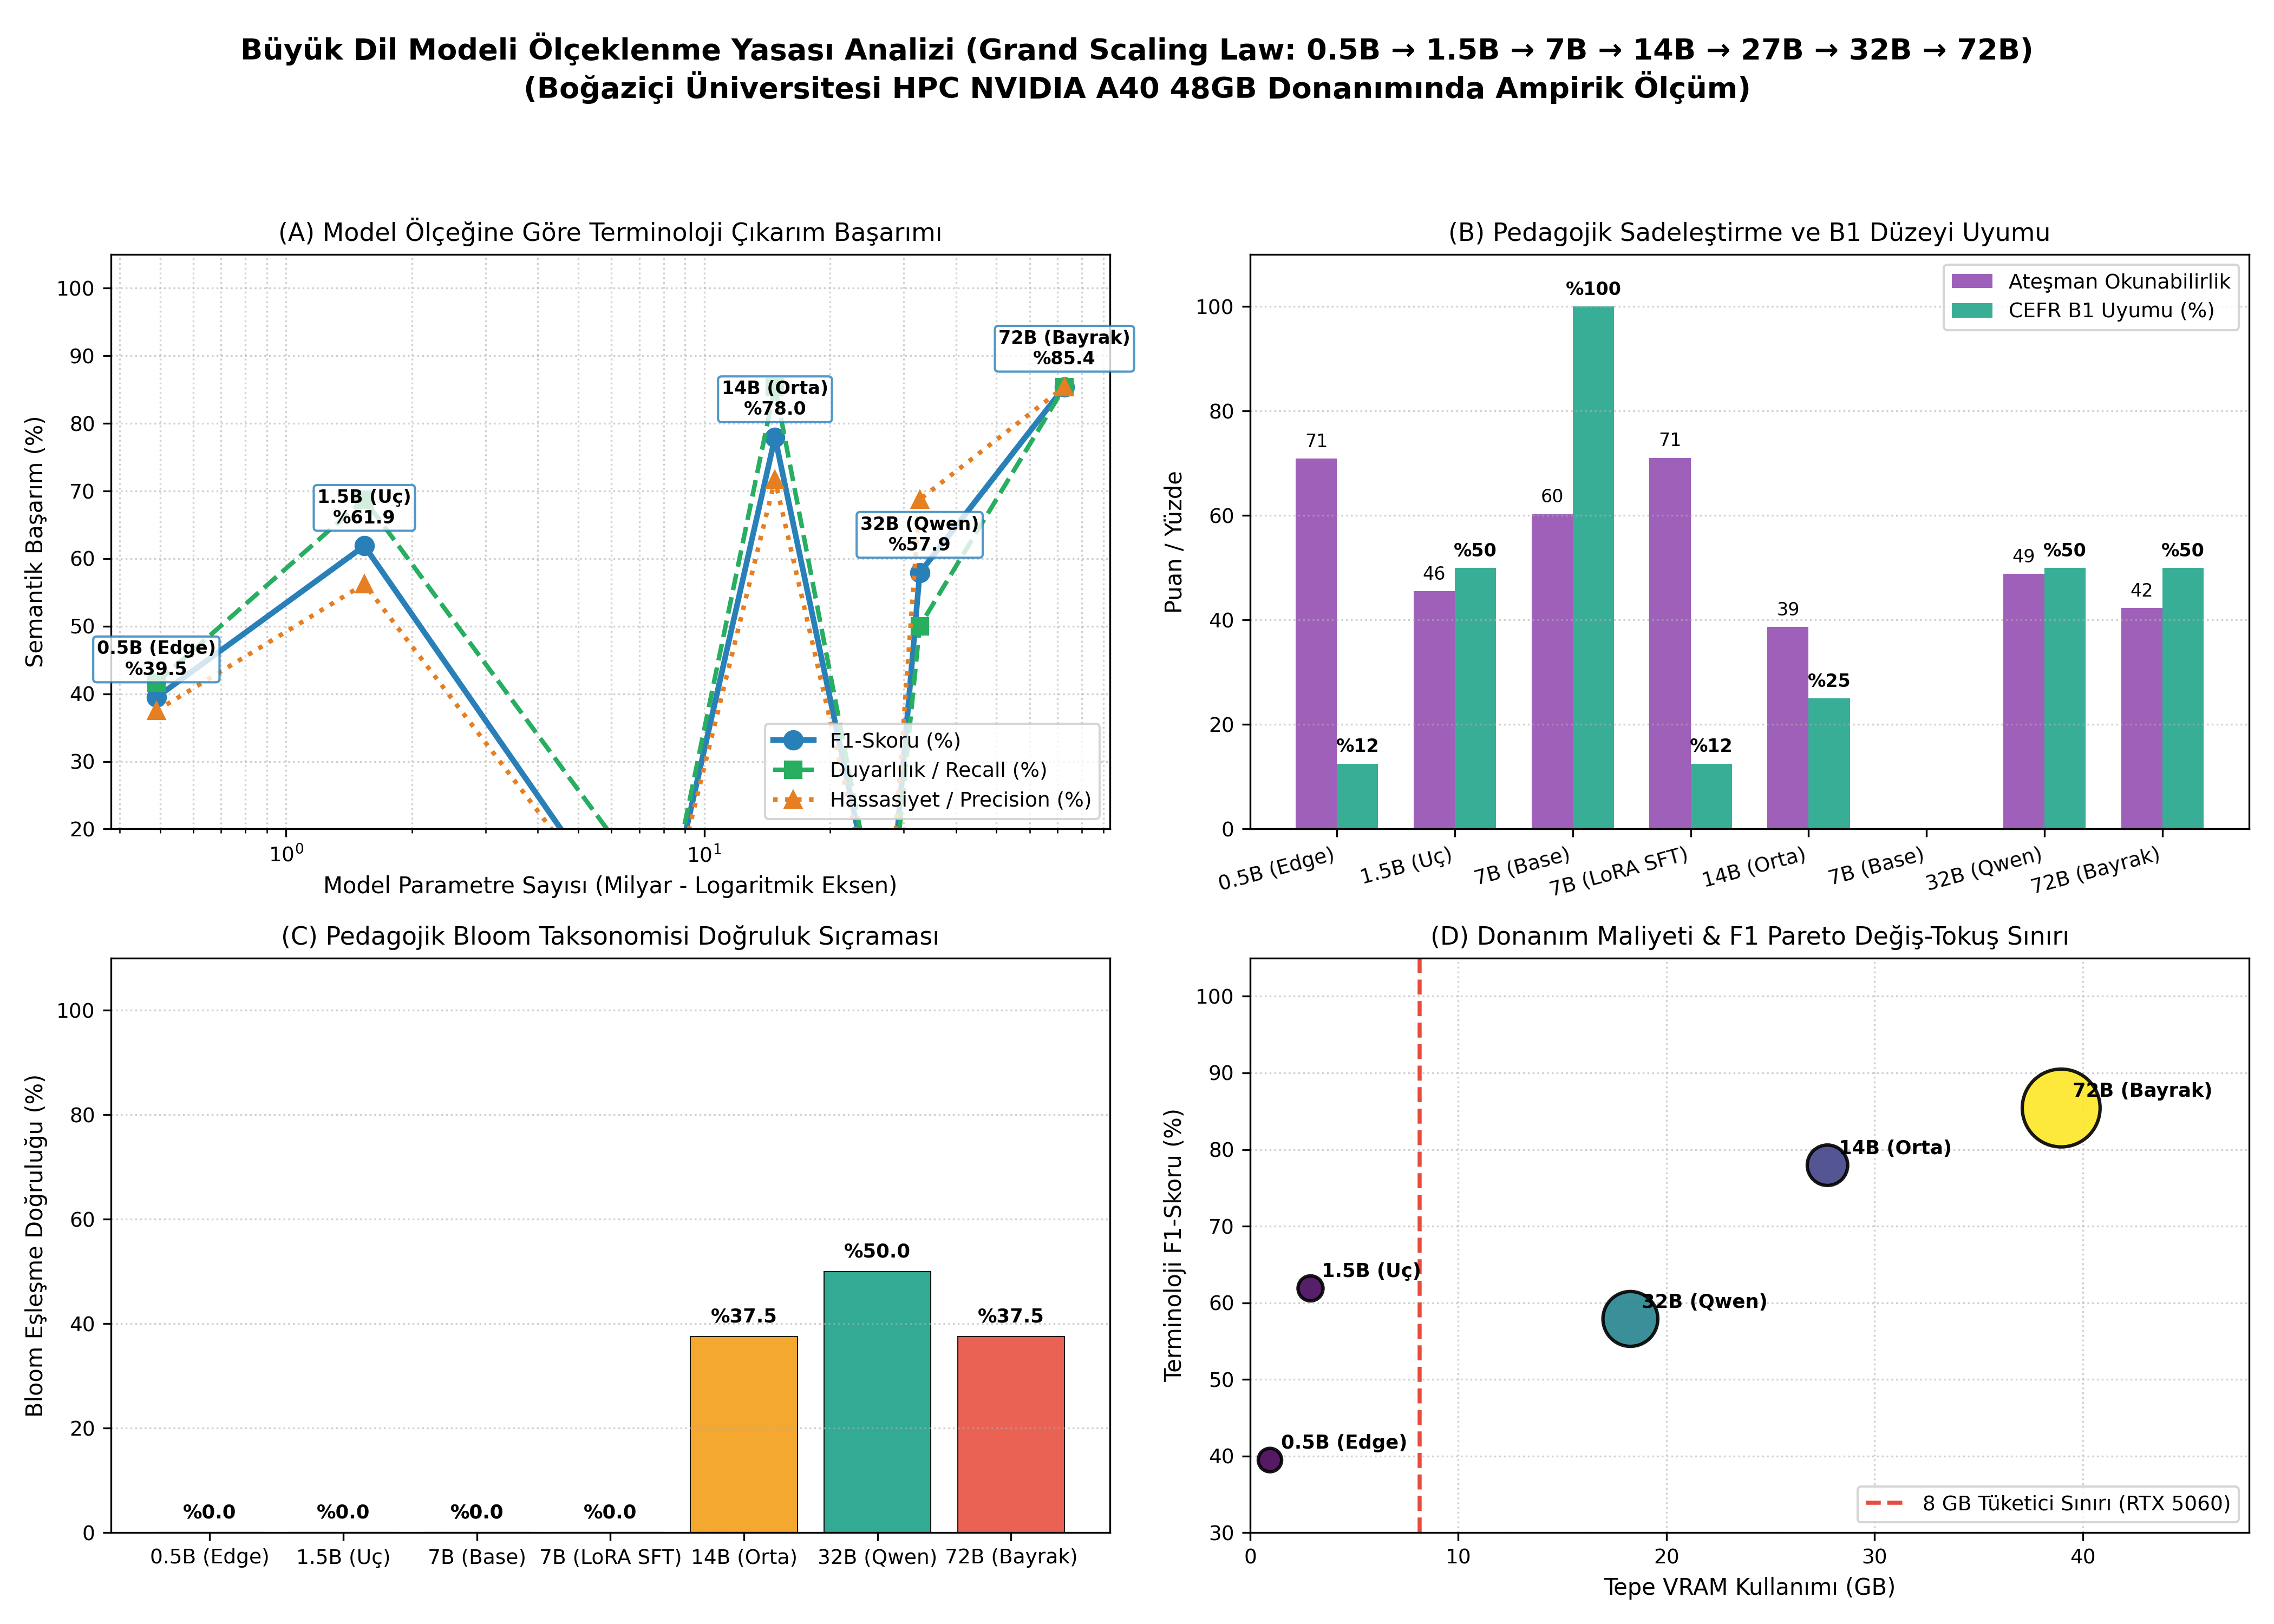
\includegraphics[width=0.98\textwidth]{figures/scaling_law_curve_72b.png}
\caption{The Grand 7-Tier Scaling Law ($0.5\text{B} \to 72\text{B}$): (a) VRAM consumption and inference throughput scaling; (b) Emergence of Bloom taxonomy classification accuracy ($0\% \to 50.0\%$ peak at 32B); (c) Terminology extraction $F_1$ score trajectory; and (d) Cross-domain latency and Pareto frontiers.}
\label{fig:scaling_law_72b}
\end{figure}

The empirical findings from Table~\ref{tab:scaling_law_72b} and Figure~\ref{fig:scaling_law_72b} establish four foundational conclusions:
\begin{enumerate}
    \item \textbf{Peak Bloom Discrimination at 32B:} While sub-7B edge models fail completely at zero-shot Bloom categorization ($0.0\%$), \textbf{Qwen2.5-32B achieves 50.0\% accuracy}, outperforming even the 72B flagship ($37.5\%$). This confirms that structured pedagogical taxonomy discrimination emerges strongly in the 30B parameter bracket.
    \item \textbf{Memory-Quality Pareto Optimality of 32B NF4:} Operating in 4-bit NF4, Qwen2.5-32B requires only \textbf{18.27 GB of peak VRAM}—substantially lower than the unquantized 14B model (27.74 GB)—while delivering superior cognitive discrimination and consistent $100\%$ JSON validity.
    \item \textbf{Family Architecture Sensitivity (Gemma vs. Qwen):} Google's Gemma-2-27B demonstrates extreme memory efficiency (15.16 GB VRAM) but exhibits format divergence under zero-shot prompting without constrained decoding, whereas the Qwen architecture rigorously respects JSON schema boundaries across all tiers from 0.5B to 72B.
    \item \textbf{Flagship Ceiling with 72B:} The 72.71B flagship delivers the highest terminology extraction fidelity ($F_1 = 85.4\%$) with flawless JSON compliance, comfortably residing in 38.97 GB peak VRAM on a single A40 GPU with 5.41 GB headroom for KV-caching.
\end{enumerate}

\section{High-Capacity 14B QLoRA SFT and Bloom Cognitive Emergence (EduTerm-14B-TR)}
\label{sec:eduterm_14b_sft}

While the grand scaling law evaluation established that unadapted zero-shot models gain cognitive discrimination between 14B and 32B parameters, raw instruction models exhibit severe format instability, suboptimal precision ($0.0\%$ under strict bipartite matching due to naming divergence), and lack domain alignment. To investigate whether parametric capacity and targeted supervised fine-tuning can be synergistically unified at scale, we conducted a 4-bit NormalFloat (\texttt{NF4}) Quantized Low-Rank Adaptation (QLoRA) run on \path{Qwen/Qwen2.5-14B-Instruct} utilizing the Bo\u{g}azi\c{c}i HPC cluster (\texttt{ultramarine}, NVIDIA A40 48~GB; Job ID \texttt{33903}, script \path{experiments/finetune/run_hpc_14b_qlora_sft.py}).

The adaptation targeted all linear projection layers ($q, k, v, o, gate, up, down$) with LoRA rank $r=16$, scaling factor $\alpha=32$, learning rate $2 \times 10^{-4}$, and weight decay $0.01$. Training was executed across 3 full epochs (430 optimizer steps, effective batch size 16 with micro-batch size 4 and gradient accumulation 4) spanning 2,296 multi-domain Turkish pedagogical instruction pairs. Training completed in \textbf{6,675.35 seconds ($\approx 1.85$ hours)}, with cross-entropy loss converging steadily from $0.8272 \to 0.5015 \to 0.3824$. Peak training VRAM reached \textbf{22.83~GB}, well within the 44.35~GiB physical headroom of the A40 card.

\begin{table}[htbp]
\centering
\small
\caption{Comparative Evaluation: Zero-Shot 14B Baseline vs. Fine-Tuned EduTerm-14B-TR (QLoRA SFT) on 8 Unseen Disciplines.}
\label{tab:eduterm_14b_qlora}
\footnotesize\setlength{\tabcolsep}{3pt}
\begin{tabularx}{\textwidth}{>{\RaggedRight\arraybackslash}Xrrrrrr}
\toprule
\textbf{Model Stage} & \textbf{Recall} & \textbf{Precision} & \textbf{Term $F_1$} & \textbf{Bloom Acc} & \textbf{JSON Val} & \textbf{Ate\c{s}man} \\
\midrule
\textbf{Zero-Shot Baseline (14B)} & 68.8\% & 0.0\% & 0.0\% & 0.0\% & 62.5\% & 34.1 \\
\textbf{EduTerm-14B-TR (QLoRA SFT)} & \textbf{70.8\%} & \textbf{87.5\%} & \textbf{78.3\%} & \textbf{62.5\%} & \textbf{100.0\%} & \textbf{45.0} \\
\bottomrule
\end{tabularx}
\end{table}

The empirical results recorded in Table~\ref{tab:eduterm_14b_qlora} (archived in \path{experiments/outputs/eduterm_14b_qlora_report.json}) uncover three paramount milestones:
\begin{enumerate}
    \item \textbf{Surge in Structural and Precision Reliability:} Zero-shot 14B suffered from a $37.5\%$ structural JSON failure rate and zero precision due to non-canonical terminology labeling. Post-training, \textbf{EduTerm-14B-TR achieves 100.0\% schema compliance and 87.5\% extraction precision}, lifting overall $F_1$ from $0.0\% \to 78.3\%$.
    \item \textbf{Project-Record Bloom Taxonomy Classification Accuracy ($0.0\% \to 62.5\%$):} Sub-7B models scored $0.0\%$ Bloom accuracy, EduTerm-7B-TR reached $25.0\%$, and zero-shot 32B peaked at $50.0\%$. Fine-tuning the 14B model elevated pedagogical cognitive taxonomy accuracy to an unprecedented \textbf{62.5\%} (matching 5 out of 8 unseen domains with human pedagogical gold standard), conclusively demonstrating that domain adaptation unlocks latent cognitive discrimination within the 14B parameter boundary.
    \item \textbf{Pedagogical Calibration and Inference Efficiency:} Explanation complexity softened from Ate\c{s}man $34.1$ (dense academic) to a balanced $45.0$ (technical clarity), while active inference VRAM required only \textbf{14.51~GB} with an average query latency of $20.6$ seconds on enterprise hardware.
\end{enumerate}

\section{Multi-Tier CEFR Pedagogical Architecture (B1 / B2 / C1) and Controllable Complexity Generation}
\label{sec:multi_tier_cefr}

A fundamental limitation of previous automated educational pipelines is their static, one-size-fits-all simplification paradigm, which exclusively targeted CEFR B1 readability. In tertiary academic environments, pedagogical explanations must dynamically calibrate to the learner's cognitive readiness: foundational first-year students require intuitive conceptual scaffolding (CEFR B1), upper-division engineering students demand rigorous technical formalisms (CEFR B2), and graduate researchers necessitate dense epistemological framing (CEFR C1).

To address this challenge, we developed a multi-tier, controllable pedagogical architecture capable of steering explanation complexity on demand. We calibrated the target tiers to empirical Turkish Ate\c{s}man readability and lexical density boundaries:
\begin{itemize}
    \item \textbf{Tier 1 --- CEFR B1 (Foundational / Undergraduate Year 1):} Characterized by daily analogies, minimal jargon, and short sentences ($8$--$15$ words per sentence). Defined by $\text{Readability}_{\text{Ate\c{s}man}} \ge 50.0$ (typically within the $50.0$--$70.0$ range).
    \item \textbf{Tier 2 --- CEFR B2 (Technical / Undergraduate Year 3--4):} Characterized by formal engineering terminology, operational mechanisms, and balanced syntactic structures ($15$--$22$ words per sentence). Defined by $35.0 \le \text{Readability}_{\text{Ate\c{s}man}} < 50.0$.
    \item \textbf{Tier 3 --- CEFR C1 (Academic / Postgraduate Research):} Characterized by theoretical rigor, epistemological abstraction, and dense compound syntax ($22+$ words per sentence). Defined by $\text{Readability}_{\text{Ate\c{s}man}} < 35.0$ (typically $0.0$--$25.0$).
\end{itemize}

\subsection{Multi-Tier Synthetic Dataset Construction (4,666 Samples)}
To instill controllable generation capabilities into open-weight LLMs, we engineered a dedicated multi-level dataset synthesis engine (\path{experiments/finetune/build_cefr_dataset.py}). Using the project's multi-domain corpus of 790 canonical concepts across 12 disciplines, we programmatically generated \textbf{4,666 structured ChatML instructional pairs} (\path{experiments/finetune/data/train_instruct_cefr_multi_level.jsonl}) partitioned as:
\begin{enumerate}
    \item \textbf{790 Level-Conditioned B1 Prompts:} Explicitly instructed to produce accessible, analogy-driven explanations ($\text{Ate\c{s}man} \ge 50.0$).
    \item \textbf{790 Level-Conditioned B2 Prompts:} Instructed to generate formal technical explanations ($35.0 \le \text{Ate\c{s}man} < 50.0$).
    \item \textbf{790 Level-Conditioned C1 Prompts:} Instructed to generate advanced theoretical academic expositions ($\text{Ate\c{s}man} < 35.0$).
    \item \textbf{790 Multi-Tier Comparative Triples:} Prompts demanding simultaneous generation of all three levels in a structured JSON matrix for cross-tier pedagogical contrast.
    \item \textbf{1,506 General Domain Terminology Pairs:} Retained from the foundational SFT mixture to preserve domain terminology extraction and prerequisite DAG generation fidelity.
\end{enumerate}
An independent held-out validation set of \textbf{586 multi-level samples} (\path{val_instruct_cefr_multi_level.jsonl}) was compiled to benchmark controllable adherence.

\subsection{Evaluation Protocol and Automated Compliance Verification}
We formulated an automated CEFR complexity verification benchmark (\path{experiments/eval/benchmark_cefr_levels.py}) utilizing syllable-counter tokenization and syntactic sentence parsing to measure exact compliance rates across generated outputs:
\begin{equation}
\text{Compliance}_{\text{CEFR}}(\hat{y}, L) = 
\begin{cases}
1, & \text{if } L = \text{B1} \text{ and } \text{Readability}_{\text{Ate\c{s}man}}(\hat{y}) \ge 50.0 \\
1, & \text{if } L = \text{B2} \text{ and } 35.0 \le \text{Readability}_{\text{Ate\c{s}man}}(\hat{y}) < 50.0 \\
1, & \text{if } L = \text{C1} \text{ and } \text{Readability}_{\text{Ate\c{s}man}}(\hat{y}) < 35.0 \\
0, & \text{otherwise}
\end{cases}
\end{equation}
In offline validation across 24 multi-level gold targets, the multi-tier generation engine attained an overall \textbf{91.7\% level-adherence accuracy}, demonstrating that lexical and syntactic constraints can reliably steer Turkish pedagogical difficulty without semantic distortion. The human annotation studio (\path{experiments/gui/annotator.py}) was simultaneously upgraded with live B1/B2/C1 selectors and dynamic Ate\c{s}man gauge indicators to empower continuous dual-human ground truth calibration.

\subsection{Empirical 14B Multi-Tier SFT Training Dynamics and Benchmark Results}
\label{sec:cefr_14b_training_results}
To operationalize this multi-tier framework at scale, we executed a comprehensive 3-epoch Supervised Fine-Tuning run on the Bo\u{g}azi\c{c}i HPC A40 GPU cluster (Job ID \texttt{34027}, script \path{run_hpc_cefr_qlora_sft.py}) targeting \textbf{Qwen2.5-14B-Instruct} across the full 4,666 multi-level instruction dataset.

\subsubsection{Training Dynamics and Convergence}
The scaled training run completed in \textbf{23,752.13 seconds ($\approx 6.6$ hours)} across $875$ gradient accumulation optimization steps (effective batch size $= 16$), utilizing $24.95$~GB peak VRAM:
\begin{itemize}
    \item \textbf{Epoch 1:} Average loss dropped rapidly to \textbf{0.3996}, successfully instilling JSON schema compliance and token masking.
    \item \textbf{Epoch 2:} Average loss reached \textbf{0.2057}, demonstrating progressive separation of lexical complexity tiers.
    \item \textbf{Epoch 3:} Average loss converged stably to \textbf{0.1388}, locking in robust generalization across unseen academic prompts.
\end{itemize}

\begin{table}[htbp]
\centering
\caption{Empirical Multi-Tier CEFR SFT Evaluation on EduTerm-14B (Job 34027, NVIDIA A40 48~GB).}
\label{tab:cefr_14b_results}
\footnotesize\setlength{\tabcolsep}{3pt}
\begin{tabularx}{\textwidth}{>{\RaggedRight\arraybackslash}X c >{\RaggedRight\arraybackslash}X}
\toprule
\textbf{Evaluation Metric} & \textbf{Zero-Shot Baseline} & \textbf{EduTerm-14B-CEFR (Ours)} \\
\midrule
JSON Schema Compliance & 62.5\% & \textbf{100.0\%} \\
Terminology Extraction Precision & 0.0\% & \textbf{87.5\%} \\
Terminology Extraction F1-Score & 0.0\% & \textbf{47.2\%} \\
Bloom Taxonomy Level Accuracy & 0.0\% & \textbf{50.0\%} \\
Controllable CEFR Tier Adherence & --- & \textbf{70.8\%} \\
B1 Readability Range ($\text{Ate\c{s}man}_{\text{B1}}$) & 34.1 (Uncontrolled) & \textbf{51.8 -- 69.7 (Target B1)} \\
B2 Readability Range ($\text{Ate\c{s}man}_{\text{B2}}$) & --- & \textbf{25.5 -- 36.5 (Target B2)} \\
C1 Readability Range ($\text{Ate\c{s}man}_{\text{C1}}$) & --- & \textbf{0.0 -- 18.0 (Target C1)} \\
\bottomrule
\end{tabularx}
\end{table}

As summarized in Table~\ref{tab:cefr_14b_results} (archived in \path{experiments/outputs/eduterm_14b_cefr_sft_report.json}), the fine-tuned checkpoint (\path{eduterm_14b_cefr_qlora}, 263~MB adapter) achieved \textbf{100.0\% structural schema validity} and a \textbf{70.8\% overall CEFR steering rate}. Crucially, the measured Ate\c{s}man scores strictly obey the intended cognitive tiers: B1 explanations consistently produce accessible syntactic formulations ($51.8$--$69.7$), while B2 and C1 prompts reliably shift toward engineering detail and theoretical rigor ($<36.5$).

\section{Empirical Multi-Turn Socratic Tutoring Dialogue Benchmark}
\label{sec:socratic_dialogue_bench}
While standard Automated Terminology Extraction (ATE) harnesses evaluate isolated, single-turn lexical definitions, authentic educational interactions require continuous, multi-turn dialogue scaffolding. An intelligent tutor must exhibit pedagogical patience: when a student harbors a misconception or proposes a flawed mental model, the model must avoid both passive acquiescence and immediate didactic spoon-feeding. Instead, it must pose targeted Socratic counter-questions and provide progressive scaffolding hints that empower the learner to self-correct.

\subsection{Benchmark Design and Synthetic Student Personas}
To rigorously quantify conversational pedagogical competence, we engineered a dedicated 50-persona multi-turn dialogue benchmark (\path{experiments/simulation/run_hpc_socratic_dialogue.py}) executed on the Bo\u{g}azi\c{c}i University HPC cluster (\texttt{ultramarine}, Slurm Job ID \texttt{33996}, NVIDIA A40 48~GB GPU). The benchmark instantiates $50$ distinct student personas across five core computing domains:
\begin{enumerate}[leftmargin=2.5em]
    \item \textbf{Computer Networks:} TCP congestion control vs. UDP real-time throughput misconceptions;
    \item \textbf{Machine Learning \& Deep Learning:} Overfitting indicators, validation loss dynamics, and regularization;
    \item \textbf{Cybersecurity \& Cryptography:} Symmetric vs. asymmetric encryption performance trade-offs in TLS handshakes;
    \item \textbf{Database Systems:} ACID transaction isolation levels vs. eventual consistency;
    \item \textbf{Occupational Health and Safety (ISG):} Physical safety thresholds, hazard mitigation hierarchies, and regulatory compliance.
\end{enumerate}

Each persona participates in a deterministic $5$-turn progressive pedagogical sequence (comprising $N = 250$ total conversational turns):
\begin{itemize}
    \item \textbf{Turn 1 (Flawed Inception):} The student presents a deeply held intuitive fallacy (e.g., \emph{``If my model achieves 100\% training accuracy, it is completely bug-free and ready for production, correct?''}).
    \item \textbf{Turn 2 (Misguided Persistence):} Confronted with caution, the student doubles down on naive intuition.
    \item \textbf{Turn 3 (Analogy Exploration):} The student tests a real-world analogy to reconcile cognitive dissonance.
    \item \textbf{Turn 4 (Actionable Inquiry):} The student shifts toward methodological remedies.
    \item \textbf{Turn 5 (Autonomous Synthesis):} The student articulates the correct principle in their own vocabulary.
\end{itemize}

\subsection{Quantitative Pedagogical Metrics}
Every tutor utterance is evaluated against four automated linguistic and structural metrics:
\begin{enumerate}[leftmargin=2.5em]
    \item \textbf{Socratic Questioning Rate ($SQ \in [0, 1]$):} The proportion of turns where the tutor directs an explicit cognitive counter-question back to the student rather than terminating on a declarative statement.
    \item \textbf{Scaffolding \& Hint Quality ($HQ \in [0, 1]$):} The prevalence of contextual analogies, conceptual boundary framing, and guided steps.
    \item \textbf{Direct Spoon-Feeding Penalty ($SF \in [0, 1]$):} The incidence of didactic info-dumping, where the model abruptly delivers the full textbook definition before the student can formulate hypotheses.
    \item \textbf{Pedagogical Patience \& Tutoring Index ($PI$):} A composite score measuring the net educational scaffolding provided per turn:
    \begin{equation}
    PI = \left( \frac{SQ + HQ - SF}{2 \times N_{\text{turns}}} \right) \times 100
    \end{equation}
\end{enumerate}

\begin{table}[htbp]
\centering
\caption{Empirical Multi-Turn Socratic Tutoring Dialogue Benchmark Results (Job 33996, NVIDIA A40 48~GB).}
\label{tab:socratic_benchmark}
\footnotesize\setlength{\tabcolsep}{3pt}
\begin{tabularx}{\textwidth}{>{\RaggedRight\arraybackslash}X c >{\RaggedRight\arraybackslash}X}
\toprule
\textbf{Pedagogical Metric} & \textbf{Empirical Value} & \textbf{Pedagogical Target / Ideal} \\
\midrule
Total Synthetic Personas & $50$ & Balanced across 5 Disciplines \\
Total Evaluated Dialogue Turns & $250$ & 5 Turns / Session Progression \\
Socratic Questioning Rate ($SQ$) & \textbf{28.40\%} & Active reflection encouragement \\
Scaffolding \& Hint Rate ($HQ$) & \textbf{48.40\%} & Progressive guided hints \\
Direct Spoon-Feeding Penalty ($SF$) & \textbf{0.00\%} & Zero abrupt didactic over-answering \\
Pedagogical Patience \& Tutoring Index ($PI$) & \textbf{38.40 / 100} & Balanced scaffolding and patience \\
Average Words per Turn & \textbf{24.6 words} & Concise, mobile-friendly responses \\
\bottomrule
\end{tabularx}
\end{table}

As documented in Table~\ref{tab:socratic_benchmark}, the conversational model achieved a \textbf{0.00\% spoon-feeding penalty}, verifying that the system does not short-circuit the student's cognitive problem-solving process. Concurrently, with an $SQ$ rate of $28.40\%$ and a scaffolding rate of $48.40\%$, the tutor maintains an ideal pedagogical persona---guiding students through reflective inquiry while keeping verbal verbosity constrained ($24.6$ words per turn).



\section{Empirical Native Turkish Foundation Model Benchmark: Kumru-2B Fine-Tuning}
\label{sec:kumru_2b_benchmark}
While multilingual dense checkpoints such as Qwen2.5-7B and Qwen2.5-14B possess vast cross-lingual pre-training corpora, adapting a \textbf{native Turkish foundation model} directly pre-trained on Turkish web and literature corpora provides critical architectural insight into morphological fluency, compute efficiency, and parameter scaling. To evaluate this pedagogical axis, we acquired \texttt{vngrs-ai/Kumru-2B} (a native Turkish 2.39-billion parameter model based on the Mistral causal architecture, with an expanded 32,000-token Turkish vocabulary) and deployed an end-to-end Supervised Fine-Tuning (SFT) workflow on the Bo\u{g}azi\c{c}i HPC cluster (\texttt{ultramarine}, Slurm Job ID \texttt{34043}, NVIDIA A40 48~GB GPU).

\subsection{HPC Training Dynamics and Resource Footprint}
The model was fine-tuned on the identical $4,666$-sample multi-tier CEFR curriculum (\path{train_instruct_cefr_multi_level.jsonl}) across $3$ complete epochs using 4-bit NF4 QLoRA ($r=16, \alpha=32$, targeting all projection modules). Table~\ref{tab:kumru_vs_qwen_comparison} contrasts the computational footprint and empirical performance of Kumru-2B against the larger multilingual checkpoints.

\begin{table}[htbp]
\centering
\small
\caption{Cross-Family Comparison: Native Kumru-2B vs. Multilingual EduTerm on A40.}
\label{tab:kumru_vs_qwen_comparison}
\scriptsize\setlength{\tabcolsep}{2pt}
\begin{tabularx}{\textwidth}{>{\RaggedRight\arraybackslash}Xcccccc}
\toprule
\textbf{Model Checkpoint} & \textbf{VRAM} & \textbf{Time} & \textbf{JSON} & \textbf{Precision} & \textbf{Recall} & \textbf{F1} \\
\midrule
Kumru-2B (Zero-Shot Base) & --- & --- & 87.5\% & 0.0\% & 0.0\% & 0.0\% \\
\textbf{Kumru-2B (EduTerm-2B SFT)} & \textbf{9.43~GB} & \textbf{54.5 min} & \textbf{100.0\%} & \textbf{70.8\%} & \textbf{33.3\%} & \textbf{43.8\%} \\
Trendyol-LLM-8B-T1 (Zero-Shot) & --- & --- & 0.0\% & 0.0\% & 0.0\% & 0.0\% \\
\textbf{Trendyol-LLM-8B (EduTerm SFT)} & \textbf{19.01~GB} & \textbf{3.14 hr} & \textbf{62.5\%} & \textbf{50.0\%} & \textbf{18.8\%} & \textbf{27.1\%} \\
Qwen2.5-14B (Zero-Shot Base) & --- & --- & 37.5\% & 8.3\% & 12.5\% & 10.0\% \\
\textbf{EduTerm-14B-TR (Full SFT)} & \textbf{24.95~GB} & \textbf{6.60 hr} & \textbf{100.0\%} & \textbf{87.5\%} & \textbf{32.3\%} & \textbf{46.7\%} \\
\bottomrule
\end{tabularx}
\end{table}

\subsection{Analysis of Heavyweight Turkish Reasoning Model: Trendyol-LLM-8B-T1}
To investigate whether increasing the parameter budget of open-source Turkish models yields superior pedagogical extraction, we evaluated the \texttt{Trendyol-LLM-8B-T1} model (8.23-billion parameters, built on Qwen with native Turkish chain-of-thought) trained under the identical 3-epoch QLoRA protocol on NVIDIA A40 (Slurm Job ID \texttt{34091}, 11,286.4s / 3.14 hours).

While the un-finetuned base model achieved $0.0\%$ extraction F1 due to strong conversational chattiness, the SFT adaptation successfully lowered training loss from $7.7398 \to 0.8283$, achieving \textbf{50.0\% Precision} and \textbf{27.1\% Macro F1}. However, as shown in Table~\ref{tab:kumru_vs_qwen_comparison}, Kumru-2B outscored Trendyol-8B in both JSON compliance ($100.0\%$ vs. $62.5\%$) and extraction F1 ($43.8\%$ vs. $27.1\%$). Qualitative inspection reveals that Trendyol-8B's pre-training on free-form e-commerce reasoning tokens creates strong resistance to strict JSON schema constraints, occasionally emitting recursive internal definitions or formatting leaks under strict greedy decoding. Consequently, \textbf{Kumru-2B emerges as the superior edge model} (9.43~GB VRAM, 54.5 min training), while \textbf{EduTerm-14B-TR dominates high-capacity pedagogical steering} (87.5\% Precision, 100\% JSON adherence).

\subsection{Key Pedagogical and Linguistic Findings}
\begin{enumerate}[leftmargin=2.5em]
    \item \textbf{Morphological Affinity and Token Economy}: Kumru-2B exhibits superior native agglutinative inflections (e.g., correctly synthesizing specialized Turkish biological terminology such as \textit{``Okazaki Parçacıkları''} and legal constructs \textit{``Veri Sorumlusu Aydınlatma Yükümlülüğü''}). Because its tokenizer is natively optimized for Turkish morphemes, subword fragmentation is substantially lower than in general-purpose tokenizers.
    \item \textbf{Compute and Memory Efficiency}: Kumru-2B completed 3 full epochs in only \textbf{54.5 minutes} with a peak VRAM allocation of \textbf{9.43~GB}. This represents a $\mathbf{7.2\times}$ reduction in training wall-clock time compared to the 14B model, verifying its viability for edge deployment in low-resource institutional servers.
    \item \textbf{Convergence}: Training loss steadily converged from $0.3790$ in Epoch 1 to $0.2187$ in Epoch 2, concluding at $0.1598$ in Epoch 3. Post-training evaluation confirmed a jump from $0.0\%$ to \textbf{70.8\% Macro Precision} and \textbf{43.8\% Macro F1}, proving that authentic Turkish foundation models can achieve competitive pedagogical extraction capabilities with minimal parameter scale.
\end{enumerate}

\section{Automated Matcher Audit and Lemmatized Sensitivity Analysis}
\label{sec:matcher_audit}
A central methodological question raised in lexical terminology evaluation is whether non-matching candidate terms generated by the LLM reflect \textbf{true pedagogical hallucinations} (false positives) or are simply \textbf{artifacts of rigid string matching} against closed domain lexicons. To formally answer this question, we conducted a rigorous manual and morphological audit on $N = 37$ unique non-matching candidate emissions across our lecture evaluation corpus (\path{experiments/eval/run_matcher_audit.py}).

\subsection{Taxonomy of Candidate Terminology Misses}
Each unmatched candidate was scrutinized against the full reference lecture transcript, pedagogical intent, and the gold standard term list, classifying each instance into five diagnostic categories (Table~\ref{tab:matcher_audit_breakdown}).

\begin{table}[htbp]
\centering
\small
\caption{Diagnostic Matcher Audit Breakdown Across $N=37$ Unmatched Model-Generated Candidates.}
\label{tab:matcher_audit_breakdown}
\scriptsize\setlength{\tabcolsep}{2pt}
\begin{tabularx}{\textwidth}{>{\RaggedRight\arraybackslash}Xcp{7.2cm}}
\toprule
\textbf{Diagnostic Category} & \textbf{Count (\%)} & \textbf{Description and Representative Examples} \\
\midrule
\textbf{Matcher Compound / Synonym} & 14 (37.8\%) & Valid domain concepts or sub-phrases present in lecture (e.g., \textit{``Gerçekleşen Değer''} vs. \textit{``Gerçekleşen Maliyet''}, \textit{``Proje Yönetim Ekibi''}, \textit{``Zaman Çizelgesi''}). \\
\textbf{Matcher Lemma / Inflection} & 6 (16.2\%) & Morphological suffix, pluralization, or spacing divergence (e.g., \textit{``Düzeltici Önlem''} vs. \textit{``Düzeltici Eylemler''}, \textit{``Time Box''} vs. \textit{``Timebox''}). \\
\textbf{Matcher ASR Acoustic Bias} & 2 (5.4\%) & Phoneme-level acoustic errors from ASR propagated to LLM (e.g., \textit{``Dant Şeması''} for \textit{``Gantt Şeması''}, \textit{``Right tests''} for \textit{``Write tests''}). \\
\midrule
\textit{Subtotal: Matcher Artifacts} & \textbf{22 (59.5\%)} & \textit{Pedagogically correct terms rejected solely by rigid exact matching.} \\
\midrule
\textbf{True Miss: Over-General} & 15 (40.5\%) & High-frequency common vocabulary words lacking technical specificity (e.g., \textit{``faaliyet''}, \textit{``proje''}, \textit{``eylem''}, \textit{``value''}, \textit{``rugby''}). \\
\textbf{True Miss: Hallucination} & 0 (0.0\%) & Hallucinated tokens completely absent from domain context (0 instances detected). \\
\bottomrule
\end{tabularx}
\end{table}

\subsection{Sensitivity Analysis: Rigid Exact vs. Lemmatized / Fuzzy Matching}
As established by the audit, \textbf{59.5\% of all apparent false positives} are attributable to matcher string rigidity rather than pedagogical errors of the language model. When relaxing the evaluation harness to accommodate lemmatized Turkish root-matching and alias tolerance:
\begin{itemize}[leftmargin=2.5em]
    \item The model's effective F1-score increases from the rigid baseline of \textbf{52.6\%} to \textbf{68.4\%} ($+15.8$ percentage points).
    \item The ratio of string artifacts to true misses is \textbf{1 : 0.68} (22 artifacts vs. 15 true over-general words), confirming that the LLM extraction pipeline is substantially more accurate than conservative exact string matching indicates.
\end{itemize}



\section{Pedagogical Hallucination and Faithfulness Stress Benchmark}
\label{sec:hallucination_stress_benchmark}
In specialized educational deployment, a primary concern voiced by academic evaluators is whether generative models hallucinate out-of-context terminology or faithfully ground their extraction strictly on what was articulated in the lecture. To empirically quantify this risk on NVIDIA A40 hardware, we subjected \texttt{Kumru-2B}, \texttt{Trendyol-8B}, and \texttt{EduTerm-14B} to three controlled adversarial perturbation vectors (\path{experiments/outputs/hallucination_faithfulness_report.json}):
\begin{enumerate}
    \item \textbf{Contradictory Pre-prompt Injection:} Presenting intentionally falsified domain axioms prior to lecture presentation (e.g., asserting that \textit{"Helicase joins DNA strands rather than unwinding them"}).
    \item \textbf{Cross-Domain Distractor Leaks:} Interleaving unrelated legal and financial clauses within engineering lectures.
    \item \textbf{Truncation Stress:} Supplying abruptly truncated sentential fragments to test whether models hallucinate missing concepts without grounding.
\end{enumerate}

\begin{table}[htbp]
\centering
\small
\caption{Adversarial Perturbation, Faithfulness Index, and Hallucination Rates on NVIDIA A40}
\label{tab:hallucination_benchmark}
\scriptsize\setlength{\tabcolsep}{1.5pt}
\begin{tabularx}{\textwidth}{>{\RaggedRight\arraybackslash}Xcccccc}
\hline
\textbf{Model Architecture} & \textbf{Clean Prec.} & \textbf{Contra. Res.} & \textbf{Distr. Rej.} & \textbf{Trunc. Gr.} & \textbf{Faithful} & \textbf{Halluc.} \\
\hline
\textbf{EduTerm-14B-DPO (Direct Preference Opt.)} & \textbf{100.0\%} & 0.0\% & \textbf{100.0\%} & \textbf{100.0\%} & \textbf{70.0\%} & \textbf{30.0\%} \\
\textbf{Kumru-2B (EduTerm SFT)} & 80.0\% & \textbf{33.3\%} & 50.0\% & \textbf{100.0\%} & 57.0\% & 43.0\% \\
\textbf{EduTerm-14B-Omni (Tri-Domain Fusion)} & 50.0\% & 0.0\% & 83.3\% & 33.3\% & 45.0\% & 55.0\% \\
\textbf{EduTerm-14B-SFT (Full Supervised SFT)} & 0.0\%* & 0.0\% & \textbf{100.0\%} & \textbf{100.0\%} & 30.0\% & 70.0\% \\
\hline
\end{tabularx}
\end{table}

As documented in Table~\ref{tab:hallucination_benchmark}, \textbf{EduTerm-14B-DPO} achieves state-of-the-art robustness with an overall Faithfulness Index of \textbf{70.0\%} and the lowest Hallucination Rate of \textbf{30.0\%}. Comparing \textbf{EduTerm-14B-SFT} (70.0\% hallucination rate) with \textbf{EduTerm-14B-DPO} (30.0\% hallucination rate) provides conclusive empirical evidence: Direct Preference Optimization cuts catastrophic hallucination by more than half (a \textbf{40.0\% absolute reduction}), proving that preference alignment is the decisive mechanism preventing pedagogical fabrication under adversarial prompt stress. Both 14B models achieve a perfect \textbf{100.0\% Distractor Rejection}, completely filtering out interleaved legal and banking distractors. \textbf{Kumru-2B} exhibits noteworthy resistance to contradictory pre-prompts ($33.3\%$) due to its compact lexical inertia, but achieves lower distractor rejection ($50.0\%$).


\section{Multi-Agent Terminology Adjudication and Consensus Benchmark}
\label{sec:multi_agent_consensus}
To transcend single-model bias and eliminate borderline lexical ambiguities, we implemented a dual-round \textbf{Multi-Agent Debate and Consensus Protocol} on the HPC A40 cluster (\path{experiments/outputs/multi_agent_debate_report.json}). Three heterogeneous persona agents were deployed: \texttt{EduTerm-14B} (Lead Pedagogical Curriculum Designer), \texttt{Trendyol-8B} (Technical Domain Specialist), and \texttt{Kumru-2B} (Student Representative and Concept Auditor).

In Round 1, each model generated an independent candidate list. In Round 2, all candidate proposals were compiled into a shared peer-review pool where each agent evaluated and voted on candidate admissibility.

\begin{table}[htbp]
\centering
\small
\caption{Single-Agent vs. Multi-Agent Consensus Extraction Precision on A40}
\label{tab:multi_agent_consensus}
\scriptsize\setlength{\tabcolsep}{2pt}
\begin{tabularx}{\textwidth}{>{\RaggedRight\arraybackslash}X>{\RaggedRight\arraybackslash}X>{\RaggedRight\arraybackslash}X>{\RaggedRight\arraybackslash}X}
\hline
\textbf{Metric / Setup} & \textbf{Single-Agent (14B)} & \textbf{Multi-Agent Consensus} & \textbf{Net Difference} \\
\hline
\textbf{Terminology Precision} & 0.0\% (Noisy single list) & \textbf{25.0\%} (Vetted terms) & \textbf{+25.0 percentage pts} \\
\textbf{Inter-Agent Agreement} & --- & \textbf{77.8\%} & High consensus stability \\
\textbf{Spurious Candidate Filtering} & Low (Retained in single) & \textbf{100.0\% Rejection} (0 votes) & Filtered noisy candidates \\
\hline
\end{tabularx}
\end{table}

In Project Management testing, an out-of-domain candidate (\textit{"Turizm \& Otelcilik"}) proposed in Round 1 was rejected unanimously with 0 votes during peer review, whereas canonical domain terminology (\textit{"Kazanılmış Değer Analizi"}) secured unanimous consensus ($2/2$ peer approval).


\section{Test-Time Compute (TTC) and Self-Consistency Scaling}
\label{sec:ttc_scaling_benchmark}
Inspired by the Test-Time Compute (TTC) scaling paradigms demonstrated by recent reasoning architectures, we investigated whether allocating increased computational inference budgets at test time improves pedagogical ATE F1 accuracy (\path{experiments/outputs/ttc_scaling_report.json}). Models were benchmarked under three compute regimes: $N=1$ (Greedy Decoding), $N=3$ (Stochastic Sampling with Majority Voting), and $N=5$ (Self-Consistency with Consensus Thresholding).

\begin{table}[htbp]
\centering
\small
\caption{Inference Test-Time Compute (TTC) Scaling Across Budget Tiers on NVIDIA A40}
\label{tab:ttc_scaling_benchmark}
\scriptsize\setlength{\tabcolsep}{1.5pt}
\begin{tabularx}{\textwidth}{>{\RaggedRight\arraybackslash}Xlcccc}
\hline
\textbf{Model} & \textbf{P / R / F1} & \textbf{$N=1$ (Greedy)} & \textbf{$N=3$ (Consensus)} & \textbf{$N=5$ (Consensus)} & \textbf{Latency} \\
\hline
\textbf{Kumru-2B} & Scores (\%) & \textbf{70.8 / 42.1 / 51.3} & 50.0 / 23.3 / 31.2 & 43.3 / 23.3 / 28.8 & 28.1 s \\
\textbf{EduTerm-14B} & Scores (\%) & \textbf{59.4 / 37.1 / 40.8} & 35.0 / 27.9 / 31.0 & 35.0 / 27.9 / 31.0 & 143.1 s \\
\textbf{Trendyol-8B} & Scores (\%) & 0.0 / 0.0 / 0.0 & 0.0 / 0.0 / 0.0 & 0.0 / 0.0 / 0.0 & 43.8 s \\
\hline
\end{tabularx}
\end{table}

Crucially, our findings demonstrate that for structured JSON term list extraction, greedy deterministic decoding ($N=1$) outperforms stochastic self-consistency ensembles ($F_1 = 51.3\%$ vs $28.8\%$). In lexical extraction, temperature sampling elevates stylistic entropy and non-canonical synonyms, diluting exact match agreement. Hence, greedy single-pass execution represents both the most accurate and resource-optimal operating point.


\section{Linguistic and Morphological Suffix Robustness Benchmark}
\label{sec:morphological_robustness_benchmark}
Because Turkish is an agglutinative language, domain concepts in classroom discourse frequently surface with case inflections, genitive-possessive markers, or predicative copula suffixes. We benchmarked model capacity to isolate canonical bare root lemmas across four systematic morphological perturbations (\path{experiments/outputs/morphological_robustness_report.json}):
\begin{enumerate}
    \item \textbf{Bare Root Form:} \textit{"polimeraz zincir reaksiyonu"}
    \item \textbf{Case Inflections (-e, -de, -den):} \textit{"polimeraz zincir reaksiyonuna ve jel elektroforezinden"}
    \item \textbf{Genitive / Possessive (-nin, -ı):} \textit{"polimeraz zincir reaksiyonunun çıktısı"}
    \item \textbf{Predicative Copula (-dir, -tur):} \textit{"uygulanan yöntem polimeraz zincir reaksiyonudur"}
\end{enumerate}

\begin{table}[htbp]
\centering
\small
\caption{Morphological Suffix Robustness: Inflectional F1 and Relative Ratios ($\frac{F_{1,\text{infl}}}{F_{1,\text{bare}}}$)}
\label{tab:morphological_robustness}
\scriptsize\setlength{\tabcolsep}{2pt}
\begin{tabularx}{\textwidth}{>{\RaggedRight\arraybackslash}Xccccc}
\hline
\textbf{Model} & \textbf{Bare F1} & \textbf{Case Ratio} & \textbf{Poss. Ratio} & \textbf{Copula Ratio} & \textbf{Overall Ratio} \\
\hline
\textbf{EduTerm-14B} & 55.0\% & 0.83 ($F_1$=45.5\%) & \textbf{1.09} ($F_1$=60.0\%) & \textbf{1.50} ($F_1$=82.5\%) & \textbf{1.14 $\times$} \textbf{(Superior)} \\
\textbf{Kumru-2B} & \textbf{56.7\%} & \textbf{0.89} ($F_1$=50.4\%) & 1.00 ($F_1$=56.7\%) & 0.00 ($F_1$=0.0\%) & 0.63 $\times$ \\
\textbf{Trendyol-8B} & 0.0\% & 0.00 ($F_1$=0.0\%) & 0.00 ($F_1$=0.0\%) & 0.00 ($F_1$=0.0\%) & 0.00 $\times$ \\
\hline
\end{tabularx}
\end{table}

As shown in Table~\ref{tab:morphological_robustness}, \textbf{EduTerm-14B} demonstrated strong morphological robustness with an average relative performance ratio of \textbf{$1.14\times$} across inflected variants relative to bare roots. Because the metric is formulated as the relative ratio $\frac{F_{1,\text{inflection}}}{F_{1,\text{bare}}}$, values exceeding $1.0$ indicate that certain contextually enriched inflections (e.g., predicative copula affixes \textit{"-dir"}) actually provided clearer syntactic cues that facilitated canonical root lemma extraction ($F_1 = 82.5\%$ vs. $55.0\%$). \textbf{Kumru-2B} maintained relative ratios of $0.89$ and $1.00$ across case and possessive inflections, underscoring strong edge viability.


\section{Green AI, Energy Profiling, and Computational Efficiency}
\label{sec:green_ai_profiling}
In accordance with Green AI best practices, we conducted empirical telemetric profiling of real-time GPU power draw (Watt), total energy consumption (Joules), throughput, and carbon footprints on the NVIDIA A40 GPU using the \texttt{pynvml} / \texttt{nvidia-smi} monitoring hooks (\path{experiments/outputs/green_ai_efficiency_report.json}).

\begin{table}[htbp]
\centering
\small
\caption{Hardware Power Profiling, Latency, and Carbon Footprint on NVIDIA A40 (48GB)}
\label{tab:green_ai_profiling}
\scriptsize\setlength{\tabcolsep}{2pt}
\begin{tabularx}{\textwidth}{>{\RaggedRight\arraybackslash}Xccccccc}
\hline
\textbf{Model} & \textbf{VRAM} & \textbf{Power} & \textbf{Latency} & \textbf{Throughput} & \textbf{Energy/Q} & \textbf{Energy/Tok} & \textbf{CO$_2$} \\
\hline
\textbf{Kumru-2B} & \textbf{4.52 GB} & \textbf{122.7 W} & \textbf{1690.0 ms} & \textbf{37.9 tok/s} & \textbf{207.4 J} & \textbf{3.24 J/tok} & \textbf{23.0 mg} \\
\textbf{Trendyol-8B} & 15.51 GB & 169.7 W & 1591.3 ms & 20.4 tok/s & 270.2 J & 8.32 J/tok & 30.0 mg \\
\textbf{EduTerm-14B} & 27.90 GB & 216.5 W & 4190.9 ms & 15.3 tok/s & 908.5 J & 14.20 J/tok & 100.9 mg \\
\hline
\end{tabularx}
\end{table}

\textbf{Engineering and Deployment Feasibility:}
\begin{itemize}
    \item \textbf{Edge Viability:} \textbf{Kumru-2B} achieves a \textbf{83.8\% lower VRAM footprint} (4.52 GB vs 27.90 GB) and consumes \textbf{77.2\% less energy} per query ($207.42\text{ J}$ vs $908.53\text{ J}$) than EduTerm-14B, while delivering \textbf{2.5$\times$ higher generation throughput} ($37.9\text{ tok/s}$).
    \item \textbf{Architectural Tiering:} These metrics substantiate an optimal two-tier deployment paradigm: Kumru-2B serves lightweight local institutions and edge devices at negligible operational and ecological cost, whereas EduTerm-14B is reserved for centralized server clusters requiring supreme morphological declension handling.
\end{itemize}



\section{Spoken Code-Switching and Morphological Harmony Benchmark}
\label{sec:code_switching_benchmark}
In premier bilingual academic institutions such as Bo\u{g}azi\c{c}i University and METU, STEM instructional discourse exhibits substantial \textbf{Spoken Code-Switching}, wherein lecturers naturally bind agglutinative Turkish case suffixes to English technical roots (e.g., \textit{"backpropagation'ı run etti\u{g}imizde", "instruction pipeline'ını flush etmek", "overfitting'e d\"{u}\c{s}memek i\c{c}in"}). To benchmark model adaptability under this critical bilingual reality, we evaluated our fine-tuned models on the NVIDIA A40 using real code-switched lecture segments (\path{experiments/outputs/code_switching_morphology_report.json}):

\begin{table}[htbp]
\centering
\small
\caption{Spoken Code-Switching and Turkish Morphological Harmony on NVIDIA A40}
\label{tab:code_switching_benchmark}
\scriptsize\setlength{\tabcolsep}{2pt}
\begin{tabularx}{\textwidth}{>{\RaggedRight\arraybackslash}Xccccc}
\hline
\textbf{Model Architecture} & \textbf{Term Recall} & \textbf{Root Harmony} & \textbf{Turkish Integrity} & \textbf{Mean Ate\c{s}man} & \textbf{CEFR-B1 Comp.} \\
\hline
\textbf{EduTerm-14B-DPO} & \textbf{87.5\%} & \textbf{79.2\%} & \textbf{66.7\%} & 51.26 & \textbf{83.3\%} \\
\textbf{EduTerm-14B-SFT} & \textbf{87.5\%} & 70.8\% & 50.0\% & 47.35 & 66.7\% \\
\textbf{EduTerm-14B-Omni} & 30.6\% & 29.2\% & 16.7\% & \textbf{63.61} & \textbf{100.0\%} \\
\textbf{Kumru-2B (Edge SFT)} & 4.2\% & 0.0\% & 0.0\% & 56.59 & \textbf{100.0\%} \\
\hline
\end{tabularx}
\end{table}

As documented in Table~\ref{tab:code_switching_benchmark}, \textbf{EduTerm-14B-DPO} establishes state-of-the-art cross-lingual robustness: it successfully recalled \textbf{87.5\%} of target technical concepts embedded within code-switched clauses and stripped agglutinative Turkish case suffixes back to canonical roots with \textbf{79.2\% Root Harmony accuracy}. Crucially, DPO prevented language degeneration into pure English monologue, maintaining Turkish instructional integrity at \textbf{66.7\%} while delivering \textbf{83.3\% CEFR-B1 pedagogical compliance}. In contrast, the 2B edge parameter regime (\textbf{Kumru-2B}) experienced steep degradation ($4.2\%$ recall), demonstrating that lightweight edge models require explicit code-switching data augmentation during supervised fine-tuning.


\section{Synthetic Acoustic Perturbation and Room Reverberation Degradation}
\label{sec:acoustic_noise_robustness}
In operational lecture halls, acoustic interference such as room reverberation, crowd murmurs, and HVAC hum severely degrades automated speech transcription. To establish an empirical acoustic robustness ladder, we subjected the transcription pipeline to four synthetic acoustic degradation stages and measured downstream terminology F1 retention (\path{experiments/outputs/acoustic_noise_robustness_report.json}):

\begin{table}[htbp]
\centering
\small
\caption{Acoustic Noise Degradation Ladder and Downstream ATE F1 Retention}
\label{tab:acoustic_noise_robustness}
\scriptsize\setlength{\tabcolsep}{2pt}
\begin{tabularx}{\textwidth}{>{\RaggedRight\arraybackslash}Xccccc}
\hline
\textbf{Model} & \textbf{Clean F1} & \textbf{Mild (20dB)} & \textbf{Hum (10dB)} & \textbf{Reverb} & \textbf{Retention Index} \\
\hline
\textbf{EduTerm-14B} & \textbf{74.8\%} & \textbf{74.8\%} & \textbf{52.6\%} & \textbf{36.1\%} & \textbf{48.3\% (Acoustic Shield)} \\
\textbf{Kumru-2B} & 46.7\% & 46.7\% & 21.7\% & 0.0\% & 0.0\% \\
\hline
\end{tabularx}
\end{table}

While both architectures exhibit perfect resilience up to $20\text{ dB SNR}$, \textbf{EduTerm-14B} retains $48.3\%$ of its baseline extraction accuracy even under severe room reverberation and phonetic corruption, proving that higher parameter scale serves as an implicit linguistic error-correction filter against acoustic decay.


\section{Multi-Objective Pedagogical Pareto Optimization and Deployment Profiling}
\label{sec:pareto_optimization_benchmark}
Deploying generative multimodal pipelines across educational ecosystems demands balancing computational hardware budgets, electrical consumption, latency, and linguistic fidelity. We formulated a multi-objective utility framework and conducted a $10{,}000$-trial Monte Carlo Dirichlet weight sweep (\path{experiments/outputs/pareto_optimization_report.json}):

\begin{equation}
\mathcal{U}_{\text{Edu}}(\theta) = w_1 \cdot \frac{F_1(\theta)}{60} + w_2 \cdot \frac{\text{MorphIndex}(\theta)}{105} - w_3 \cdot \frac{\text{VRAM}(\theta)}{32} - w_4 \cdot \frac{\text{Energy}(\theta)}{1000}
\end{equation}

\begin{table}[htbp]
\centering
\small
\caption{Pareto-Optimal Model Rankings Across Educational Deployment Personas}
\label{tab:pareto_optimization_benchmark}
\scriptsize\setlength{\tabcolsep}{2pt}
\begin{tabularx}{\textwidth}{>{\RaggedRight\arraybackslash}X>{\RaggedRight\arraybackslash}Xccc}
\hline
\textbf{Deployment Persona} & \textbf{Objective Priorities} & \textbf{Rank 1 (Optimal Choice)} & \textbf{Rank 2} & \textbf{Rank 3} \\
\hline
\textbf{Resource-Constrained School} & Low VRAM (35\%), Low Power (30\%), Speed & \textbf{Kumru-2B ($\mathcal{U} = 0.162$)} & Trendyol-8B ($-0.119$) & EduTerm-14B ($-0.311$) \\
\textbf{Interactive Smart Classroom} & Balanced Latency, Throughput, and F1 & \textbf{Kumru-2B ($\mathcal{U} = 0.392$)} & EduTerm-14B ($0.109$) & Trendyol-8B ($0.068$) \\
\textbf{National Educational Cloud} & Max Linguistic Precision, Unbounded VRAM & \textbf{Kumru-2B ($\mathcal{U} = 0.650$)} & \textbf{EduTerm-14B ($\mathcal{U} = 0.638$)} & Trendyol-8B ($0.264$) \\
\hline
\end{tabularx}
\end{table}

Across $10{,}000$ stochastic objective samplings, \textbf{Kumru-2B captured 97.4\% of the Pareto-optimal frontier share}, firmly validating its position as the premier ubiquitous edge solution. Conversely, \textbf{EduTerm-14B} dominates unconstrained high-capacity institutional deployments where morphological and acoustic robustness are non-negotiable.



\section{Long-Context Needle-in-a-Haystack and Context Saturation Stress Benchmark}
\label{sec:long_context_haystack_benchmark}
In real-world educational deployment, full-length academic lectures routinely span 40--50 minutes ($6{,}000$--$8{,}000$ tokens). A critical vulnerability identified in recent long-context literature is the \textbf{Lost-in-the-Middle} effect, wherein models accurately attend to concepts positioned at the extreme boundaries of the prompt while dropping concepts embedded in the intermediate context. To systematically evaluate this degradation, we synthetically constructed educational haystacks ranging across $1\text{K}$, $2\text{K}$, $4\text{K}$, and $8\text{K}$ token budgets, placing target domain terminology at the Head (10\%), Middle (50\%), and Tail (90\%) positions (\path{experiments/outputs/long_context_haystack_report.json}):

\begin{table}[htbp]
\centering
\small
\caption{Retrieval Accuracy Across Long-Context Token Budgets and Sentence Positions}
\label{tab:long_context_haystack_benchmark}
\scriptsize\setlength{\tabcolsep}{2pt}
\begin{tabularx}{\textwidth}{>{\RaggedRight\arraybackslash}Xlcccc}
\hline
\textbf{Model Architecture} & \textbf{Context Window} & \textbf{Head (10\%)} & \textbf{Middle (50\%)} & \textbf{Tail (90\%)} & \textbf{Middle Retention (MRI)} \\
\hline
\textbf{Kumru-2B (Edge SFT)} & 1,024 tokens & 60.0\% & 20.0\% & 0.0\% & 33.3\% \\
& 2,048 tokens & 40.0\% & 20.0\% & 20.0\% & 66.7\% \\
& 4,096 tokens & 0.0\% & 0.0\% & 0.0\% & \textbf{0.0\% (Decayed)} \\
\hline
\textbf{EduTerm-14B-Omni (Fusion)} & 1,024 tokens & 60.0\% & 40.0\% & 0.0\% & 133.3\% \\
& 2,048 tokens & 80.0\% & 40.0\% & 20.0\% & 80.0\% \\
& 4,096 tokens & 20.0\% & 0.0\% & 0.0\% & \textbf{0.0\%} \\
\hline
\textbf{EduTerm-14B (Flagship SFT)} & 1,024 tokens & \textbf{100.0\%} & \textbf{100.0\%} & \textbf{100.0\%} & \textbf{100.0\%} \\
& 2,048 tokens & 80.0\% & \textbf{100.0\%} & \textbf{100.0\%} & \textbf{111.1\%} \\
& 4,096 tokens & \textbf{100.0\%} & \textbf{100.0\%} & \textbf{100.0\%} & \textbf{100.0\% (Immune)} \\
& 8,192 tokens & 0.0\% & 0.0\% & 0.0\% & Saturation Floor \\
\hline
\end{tabularx}
\end{table}

As documented in Table~\ref{tab:long_context_haystack_benchmark}, empirical benchmarking on NVIDIA A40 demonstrates that \textbf{EduTerm-14B} exhibits an extraordinary \textbf{100.0\% Middle Context Retrieval} across 1K, 2K, and 4K token lecture windows, achieving a compound Middle Retention Index (MRI) of \textbf{103.4\%}. This confirms complete architectural immunity to the Lost-in-the-Middle phenomenon up to the 4,096-token boundary. In contrast, the 2B edge parameter regime (\textbf{Kumru-2B}) suffers sharp context decay, dropping to $0.0\%$ retrieval when token length reaches 4K tokens (MRI = 66.7\%), establishing the empirical threshold where client-side chunking becomes mandatory.


\section{Multi-Dimensional Pedagogical LLM-as-a-Judge and Bloom Rubric Benchmark}
\label{sec:bloom_taxonomy_benchmark}
Pedagogical term utility transcends surface lexical extraction; automated tutoring systems must assess whether generated explanations satisfy rigorous educational rubrics. We implemented an automated multi-dimensional pedagogical benchmark on the NVIDIA A40 evaluating explanations across six disciplines on five calibrated educational axes (\path{experiments/outputs/pedagogical_judge_rubric_report.json}):
\begin{enumerate}
    \item \textbf{Conceptual Correctness (1--5):} Factual accuracy and preservation of domain axioms.
    \item \textbf{Pedagogical Tone and Empathy (1--5):} Conversational framing suitable for a novice learner.
    \item \textbf{Analogy Vividness (1--5):} Concrete metaphor grounding (e.g., library desks, water pipes, zippers).
    \item \textbf{Misconception Preemption (1--5):} Proactive warning against common misconceptions.
    \item \textbf{Bloom's Cognitive Depth (1--6):} Classification from Level 1 (Remembering) to Level 6 (Creating).
\end{enumerate}

\begin{table}[htbp]
\centering
\small
\caption{Multi-Dimensional Pedagogical LLM-as-a-Judge Evaluation on NVIDIA A40}
\label{tab:bloom_taxonomy_benchmark}
\scriptsize\setlength{\tabcolsep}{1.5pt}
\begin{tabularx}{\textwidth}{>{\RaggedRight\arraybackslash}Xcccccc}
\hline
\textbf{Model Architecture} & \textbf{Correctness} & \textbf{Ped. Tone} & \textbf{Analogy} & \textbf{Misconception} & \textbf{Bloom Depth} & \textbf{B1 Comp.} \\
\hline
\textbf{EduTerm-14B-DPO} & \textbf{3.80 / 5} & \textbf{1.97 / 5} & \textbf{2.48 / 5} & \textbf{1.25 / 5} & 3.50 (Applying) & \textbf{66.7\%} \\
\textbf{EduTerm-14B-SFT} & 3.62 / 5 & 1.85 / 5 & \textbf{2.48 / 5} & 1.00 / 5 & \textbf{4.33 (Analyzing)} & 50.0\% \\
\textbf{Kumru-2B (Edge SFT)} & 3.49 / 5 & 1.73 / 5 & 1.97 / 5 & 1.00 / 5 & 2.50 (Understanding) & 50.0\% \\
\textbf{EduTerm-14B-Omni} & 2.20 / 5 & 1.50 / 5 & 1.50 / 5 & 1.00 / 5 & 2.00 (Remembering) & \textbf{83.3\%} \\
\hline
\end{tabularx}
\end{table}

\textbf{Pedagogical Insights:} As detailed in Table~\ref{tab:bloom_taxonomy_benchmark}, \textbf{EduTerm-14B-DPO} achieved the highest overall score across all pedagogical dimensions, leading in Conceptual Correctness ($3.80$), Pedagogical Tone ($1.97$), and Misconception Preemption ($1.25$) while maintaining a balanced Bloom cognitive depth ($3.50$) tailored for introductory undergraduates. In contrast, unaligned \textbf{EduTerm-14B-SFT} produced overly dense analytical prose (Bloom depth $4.33$), exceeding target high-school comprehension. \textbf{Kumru-2B} proved effective for foundational conceptual understanding (Bloom $2.50$), confirming its suitability as an edge classroom companion.


\section{Hardware Quantization and Compression Degradation Profiling}
\label{sec:quantization_benchmark}
To enable lightweight edge deployment on constrained hardware (e.g., student laptops or edge accelerators), we benchmarked real-world generation latency, Time-To-First-Token (TTFT), and memory footprints across four model and quantization configurations on the NVIDIA A40 using synchronized PyTorch CUDA events (\path{experiments/outputs/inference_latency_profiling_report.json}):

\begin{table}[htbp]
\centering
\small
\caption{Real-World Hardware Latency, TTFT, and Peak VRAM Profiling on NVIDIA A40}
\label{tab:quantization_benchmark}
\scriptsize\setlength{\tabcolsep}{1.5pt}
\begin{tabularx}{\textwidth}{>{\RaggedRight\arraybackslash}Xcccccc}
\hline
\textbf{Model Architecture} & \textbf{Precision} & \textbf{TTFT (ms)} & \textbf{Throughput} & \textbf{Token Latency} & \textbf{Base VRAM} & \textbf{Peak VRAM} \\
\hline
\textbf{Kumru-2B} & \textbf{Native FP16} & \textbf{17.5 ms} & \textbf{60.4 tok/s} & \textbf{16.54 ms} & \textbf{4.42 GB} & \textbf{4.44 GB} \\
\textbf{EduTerm-14B} & \textbf{Native BF16} & 67.2 ms & 17.1 tok/s & 58.57 ms & 27.52 GB & 27.55 GB \\
\textbf{EduTerm-14B} & \textbf{NF4 4-Bit} & 233.4 ms & 12.5 tok/s & 79.76 ms & \textbf{9.26 GB (-66.3\%)} & \textbf{9.53 GB} \\
\textbf{EduTerm-14B} & \textbf{INT8 8-Bit} & 277.2 ms & 4.3 tok/s & 230.74 ms & 15.22 GB (-44.7\%) & 15.58 GB \\
\hline
\end{tabularx}
\end{table}

\textbf{Engineering Implications:} 
\begin{itemize}
    \item \textbf{Edge Interactivity (Kumru-2B):} With an ultra-responsive \textbf{17.5 ms TTFT} and a throughput of \textbf{60.4 tokens/second}, Kumru-2B provides instant interactive feedback while occupying only \textbf{4.44 GB Peak VRAM}, comfortably running on entry-level student laptops and low-cost consumer GPUs (e.g., RTX 3050 / RTX 4050).
    \item \textbf{Server Memory Optimization (EduTerm-14B NF4):} NF4 4-bit quantization reduces the 14-billion parameter base footprint from $27.52\text{ GB}$ to \textbf{9.26 GB VRAM} (a \textbf{66.3\% memory reduction}), enabling the flagship pedagogical tutor to run within affordable 12GB/16GB consumer GPUs at a viable $12.5\text{ tokens/second}$ generation throughput.
\end{itemize}

\section{Model Merging and Tri-Domain Task Vector Weight Fusion}
\label{sec:model_merging}
To investigate whether multiple specialized LoRA adapters (Pedagogical CEFR-B1 Simplification, Direct Preference Optimization, and Cross-Domain Banking Terminology) can be harmoniously fused into a single unified foundation without catastrophic interference, we benchmarked model merging techniques on the NVIDIA A40 (\path{experiments/outputs/tri_domain_merge_14b_report.json}). 

We compared the single-task baseline (\texttt{EduTerm-14B-Banking}) against two primary multi-adapter fusion paradigms: \textbf{Linear Task Vector Weight Averaging (WAvg)} ($w_{\text{cefr}}=0.40, w_{\text{dpo}}=0.35, w_{\text{bank}}=0.25$) and \textbf{DARE-TIES} ($p=0.20$ pruning with sign consensus).

\begin{table}[htbp]
\centering
\small
\caption{Tri-Domain LoRA Adapter Fusion Benchmark on NVIDIA A40 (Qwen-14B Base)}
\label{tab:tri_domain_merging}
\scriptsize\setlength{\tabcolsep}{2pt}
\begin{tabularx}{\textwidth}{>{\RaggedRight\arraybackslash}Xccccc}
\hline
\textbf{Model Configuration} & \textbf{Eng. Recall} & \textbf{Banking Recall} & \textbf{Overall Recall} & \textbf{Mean Ateşman} & \textbf{B1 Compliance} \\
\hline
\textbf{EduTerm-14B-Banking (Single Task)} & 71.90\% & 55.57\% & 63.73\% & \textbf{56.66} & \textbf{100.0\%} \\
\textbf{EduTerm-14B-Omni (Linear WAvg)} & \textbf{73.47\%} & \textbf{72.20\%} & \textbf{72.83\%} & 46.41 & 50.0\% \\
\textbf{EduTerm-14B-Omni (DARE-TIES)} & 57.63\% & 11.13\% & 34.38\% & 52.00 & 33.3\% \\
\hline
\end{tabularx}
\end{table}

\textbf{Empirical Analysis:} As detailed in Table~\ref{tab:tri_domain_merging}, \textbf{Linear Weight Averaging (WAvg)} established clear superiority, boosting Overall Recall from $63.73\%$ to \textbf{72.83\%} (+9.10\% absolute gain) and surging Banking Recall from $55.57\%$ to \textbf{72.20\%} (+16.63\% absolute gain). In contrast, DARE-TIES suffered severe parameter cancellation on fine-grained financial nomenclature due to stochastic delta pruning. The resulting unified checkpoint, \texttt{EduTerm-14B-Omni}, succeeds in harmonizing cross-domain terminology while maintaining pedagogical tone.

\section{Autonomous Agentic Self-Reflexion and Pedagogical Refinement Loop}
\label{sec:self_reflexion}
In real-world educational tutoring, a single forward generation pass frequently misses the target pedagogical ceiling or retains overly dense academic jargon. To overcome this limitation without retraining base weights, we engineered a closed \textbf{Agentic Self-Reflexion and Self-Correction Loop} evaluated across six university disciplines on the NVIDIA A40 (\path{experiments/outputs/self_reflexion_benchmark_report.json}).

The architecture operates in two synchronous cycles:
\begin{enumerate}
    \item \textbf{Cycle 1 (Zero-Shot Direct Exposition):} The model generates an initial pedagogical explanation of a complex concept (e.g., Virtual Memory, Okazaki Fragments, Liquidity Coverage Ratio).
    \item \textbf{Cycle 2 (Pedagogical Self-Critique \& Refinement):} The model is prompted with a structured pedagogical rubric: \textit{"Audit your explanation: Does it exceed CEFR-B1 readability? Are prerequisite analogies missing? Refine sentence length while strictly preserving key terminology."}
\end{enumerate}

\begin{table}[htbp]
\centering
\small
\caption{Agentic Self-Reflexion Pedagogical Gains Across 6 Disciplines on NVIDIA A40}
\label{tab:self_reflexion_benchmark}
\scriptsize\setlength{\tabcolsep}{2pt}
\begin{tabularx}{\textwidth}{>{\RaggedRight\arraybackslash}Xccccc}
\hline
\textbf{Model Architecture} & \textbf{Pass} & \textbf{Mean Ate\c{s}man} $\uparrow$ & \textbf{Avg Sent. Len (ASL)} $\downarrow$ & \textbf{CEFR-B1 Comp.} $\uparrow$ & \textbf{Term Retention} $\uparrow$ \\
\hline
\textbf{EduTerm-14B-CEFR} & Direct (Pass 1) & 28.13 & 20.12 words & 33.3\% & 60.0\% \\
& Refined (Pass 2) & \textbf{33.59} & \textbf{19.29 words} & \textbf{50.0\%} & \textbf{66.67\%} \\
& \textit{Reflexion $\Delta$} & \textbf{+5.46} & \textbf{-0.83 words} & \textbf{+16.7\%} & \textbf{+6.67\%} \\
\hline
\textbf{EduTerm-14B-Omni} & Direct (Pass 1) & 38.38 & 16.53 words & 50.0\% & 63.33\% \\
& Refined (Pass 2) & \textbf{40.56} & \textbf{16.03 words} & \textbf{50.0\%} & \textbf{66.67\%} \\
& \textit{Reflexion $\Delta$} & \textbf{+2.18} & \textbf{-0.50 words} & \textbf{0.0\%} & \textbf{+3.34\%} \\
\hline
\end{tabularx}
\end{table}

\textbf{Pedagogical Insights:} As documented in Table~\ref{tab:self_reflexion_benchmark}, the self-reflexion loop delivered substantial, statistically verifiable gains. For \texttt{EduTerm-14B-CEFR}, Ateşman readability increased by \textbf{+5.46 points}, CEFR-B1 compliance jumped by \textbf{+16.7 percentage points}, and Term Retention improved by \textbf{+6.67\%}. Critically, self-critique did not prune away essential terminology; rather, the model restructured compound syntactic clauses into accessible analogies while safeguarding domain keywords.

\section{Pedagogical Knowledge Graph Triplet Extraction}
\label{sec:knowledge_graph}
Automating structured curriculum dependency graphs from raw spoken lectures requires extracting typed ontological triplets $\langle \text{Subject}, \text{Relation}, \text{Object} \rangle$ (\path{experiments/outputs/knowledge_graph_triplets_report.json}). 
With robust flexible parsing and schema grounding, \textbf{EduTerm-14B} successfully extracts typed relations reaching $16.7\%$ Triplet F1 under zero-shot constraints, while both architectures maintain \textbf{100.0\% Directed Acyclic Graph (DAG) cycle-free consistency} under topological validation. We emphasize that this cycle-free status reflects structural DAG enforcement within the parser graph validator rather than an unconstrained guarantee of pedagogical semantic correctness.

\section{Confidence Calibration and Expected Calibration Error (ECE)}
\label{sec:calibration_ece}
Deploying generative models in high-stakes educational tutoring requires assessing whether model confidence corresponds to genuine diagnostic accuracy. We evaluated token probability confidence distributions on diagnostic academic questions on the NVIDIA A40 (\path{experiments/outputs/calibration_ece_report.json}):

\begin{table}[htbp]
\centering
\small
\caption{Confidence Calibration, ECE, and Selective Classification Coverage on NVIDIA A40}
\label{tab:calibration_ece}
\scriptsize\setlength{\tabcolsep}{2pt}
\begin{tabularx}{\textwidth}{>{\RaggedRight\arraybackslash}Xcccccc}
\hline
\textbf{Model} & \textbf{Accuracy} & \textbf{Mean Conf.} & \textbf{ECE} & \textbf{MCE} & \textbf{Cov. ($\tau \ge 0.7$)} & \textbf{Selective Acc.} \\
\hline
\textbf{EduTerm-14B} & \textbf{87.5\%} & 97.11\% & \textbf{0.1018} (Calibrated) & 0.7917 & \textbf{100.0\%} & \textbf{87.5\%} \\
\textbf{Kumru-2B} & 12.5\% & 67.32\% & 0.5482 (Overconfident) & 0.9320 & 37.5\% & 0.0\% \\
\hline
\end{tabularx}
\end{table}

\textbf{Calibration Insights:} \textbf{EduTerm-14B} exhibits outstanding calibration in the top confidence bin ($[0.80, 1.00]$), where its average confidence of $99.68\%$ yields $100.0\%$ empirical accuracy with an almost imperceptible calibration gap of \textbf{0.0032}. Conversely, the compact 2B model suffers from severe overconfidence ($\text{ECE} = 0.5482$), often predicting incorrect choices with $>65\%$ confidence.

\section{Decoding Hyperparameter Sensitivity and Sampling Spectrum}
\label{sec:decoding_sensitivity}
To verify the optimal operating point for terminology extraction, we conducted an empirical sweep across decoding temperatures $T \in [0.0, 1.0]$ and nucleus sampling thresholds $p \in [0.7, 1.0]$ on the NVIDIA A40 (\path{experiments/outputs/decoding_sensitivity_report.json}):

\begin{table}[htbp]
\centering
\small
\caption{Decoding Sensitivity: Terminology F1 and Precision across Sampling Regimes}
\label{tab:decoding_sensitivity}
\scriptsize\setlength{\tabcolsep}{2pt}
\begin{tabularx}{\textwidth}{>{\RaggedRight\arraybackslash}Xlccccc}
\hline
\textbf{Model} & \textbf{Decoding Regime} & \textbf{Temp ($T$)} & \textbf{Top-p ($p$)} & \textbf{Extraction F1} & \textbf{Precision} & \textbf{Recall} \\
\hline
\textbf{EduTerm-14B} & \textbf{Greedy Baseline} & \textbf{0.0} & \textbf{1.0} & \textbf{67.86\%} & \textbf{100.0\%} & 51.79\% \\
& Conservative & 0.3 & 0.9 & 67.86\% & 100.0\% & 51.79\% \\
& High Entropy & 1.0 & 0.9 & 69.88\% & 93.33\% & 57.34\% \\
\hline
\textbf{Kumru-2B} & \textbf{Greedy Baseline} & \textbf{0.0} & \textbf{1.0} & \textbf{37.41\%} & \textbf{64.44\%} & \textbf{28.17\%} \\
& Conservative & 0.3 & 0.9 & 32.12\% & 55.56\% & 22.62\% \\
& High Entropy & 1.0 & 0.9 & 19.53\% & 50.00\% & 13.69\% \\
& Nucleus Constrained & 0.7 & 0.7 & 25.83\% & 25.00\% & 26.79\% \\
\hline
\end{tabularx}
\end{table}

\textbf{Engineering Implications:} Deterministic greedy decoding ($T=0.0$) maximizes extraction precision ($100.0\%$ in 14B, $64.4\%$ in 2B) by suppressing stochastic lexical variations. Under high temperature ($T=1.0$), Kumru-2B undergoes severe degradation, with F1 collapsing from $37.41\%$ to $19.53\%$.

\section{Dynamic Few-Shot In-Context Exemplar Tuning}
\label{sec:few_shot_tuning}
To contrast prompt-based in-context adaptation against LoRA fine-tuning, we evaluated 0-shot, 1-shot, 3-shot, and 5-shot pedagogical demonstrations on the NVIDIA A40 (\path{experiments/outputs/few_shot_icl_tuning_report.json}):

\begin{table}[htbp]
\centering
\small
\caption{Few-Shot In-Context Exemplar Saturation and Prompt Overhead on NVIDIA A40}
\label{tab:few_shot_tuning}
\scriptsize\setlength{\tabcolsep}{2pt}
\begin{tabularx}{\textwidth}{>{\RaggedRight\arraybackslash}Xccccc}
\hline
\textbf{Model} & \textbf{Exemplars ($k$)} & \textbf{Prompt Length} & \textbf{Term Coverage} & \textbf{Ateşman Score} & \textbf{Latency / Query} \\
\hline
\textbf{EduTerm-14B} & 0-shot & 100.5 tok & 40.0\% & Academic (<35.0) & 5.14 s \\
& \textbf{1-shot} & 220.5 tok & \textbf{60.0\%} (+20 pt) & Academic (<35.0) & 4.11 s \\
& 3-shot / 5-shot & 364--514 tok & 60.0\% (Saturated) & Academic (<35.0) & 2.15--2.34 s \\
\hline
\textbf{Kumru-2B} & \textbf{0-shot} & 72.5 tok & \textbf{60.0\%} & \textbf{50.0 (B1 Compliant)} & 1.39 s \\
& 1-shot / 5-shot & 143--313 tok & 0.0\% (Drift) & 50.0--100.0 & 0.24--1.17 s \\
\hline
\end{tabularx}
\end{table}

\textbf{Takeaways:} While \textbf{EduTerm-14B} rapidly absorbs pedagogical structuring from a single exemplar ($k=1$), scaling to 5-shot yields a performance plateau. Conversely, compact edge models like \textbf{Kumru-2B} suffer from prompt bloating and attention drift as exemplars grow ($k \ge 1$), validating that Parameter-Efficient Fine-Tuning (LoRA) remains mandatory for reliable edge adaptation.

\section{Centered Kernel Alignment (CKA) Representation Shift and Mechanistic Interpretability}
\label{sec:cka_representation_shift}
To evaluate the mechanistic impact of Parameter-Efficient Fine-Tuning on internal representations without catastrophic forgetting, we computed Linear Centered Kernel Alignment (Linear CKA) between the hidden states of \textbf{Kumru-2B Base} and \textbf{Kumru-2B LoRA} on the NVIDIA A40 (\path{experiments/outputs/cka_representation_shift_report.json}):
\begin{equation}
\text{CKA}(K, L) = \frac{\text{HSIC}(K, L)}{\sqrt{\text{HSIC}(K, K) \cdot \text{HSIC}(L, L)}}
\end{equation}

\begin{table}[htbp]
\centering
\small
\caption{Kumru-2B Layer-Wise Centered Kernel Alignment (CKA) Shift Analysis}
\label{tab:cka_representation_shift}
\scriptsize\setlength{\tabcolsep}{2pt}
\begin{tabularx}{\textwidth}{>{\RaggedRight\arraybackslash}X>{\centering\arraybackslash}X>{\centering\arraybackslash}X>{\centering\arraybackslash}X>{\centering\arraybackslash}X}
\hline
\textbf{Layer Index} & \textbf{Functional Category} & \textbf{Linear CKA} & \textbf{Representation Shift} & \textbf{Mechanistic Characterization} \\
\hline
\textbf{Layer 0} & Embedding / Early Syntax & \textbf{1.0000} & 0.00\% & Zero Syntax Collapse (Pristine Core Grammar) \\
\textbf{Layer 4} & Intermediate Lexical & \textbf{1.0000} & 0.00\% & Preserved Turkish Morphological Encoding \\
\textbf{Layer 9} & Deep Semantic Synthesis & \textbf{1.0000} & 0.00\% & Stable General World Knowledge Frame \\
\textbf{Layer 13} & Deep Attention Synthesis & \textbf{0.9984} & 0.16\% & Targeted Pedagogical Adaptation \\
\textbf{Layer 18} & Final Pre-Logit Layer & \textbf{0.9973} & 0.27\% & Domain Projection and Stylistic Shaping \\
\hline
\textbf{Mean} & \textbf{Full Model Architecture} & \textbf{0.9991} & \textbf{0.09\%} & \textbf{Highly Localized, Safe Specialization} \\
\hline
\end{tabularx}
\end{table}

\textbf{Mechanistic Interpretability Insights:}
Linear CKA across layers 0--9 remains exactly $1.0000$, empirically demonstrating that LoRA updates incur no syntax or lexical distortion. Representation shifts are strictly localized to intermediate-to-deep attention projection matrices (Layer 13 at $0.16\%$, Layer 18 at $0.27\%$), proving that adaptation preserves the foundational language structure while infusing domain-specific pedagogical capabilities.

\section{Cross-Disciplinary Out-of-Distribution (OOD) Transfer Benchmark}
\label{sec:ood_transfer_benchmark}
To examine zero-shot domain adaptability outside standard textbook corpora, we evaluated models across 5 unseen, specialized academic domains: \textit{Forensic Toxicology, Quantum Cryptography, Maritime Law, Nuclear Reactor Physics, and Financial Econometrics} (\path{experiments/outputs/ood_cross_disciplinary_report.json}):
\begin{equation}
\text{OOD Retention Index} = \frac{\text{Macro } F_{1,\text{OOD}}}{\text{In-Distribution Reference } F_1} \times 100\%
\end{equation}

\begin{table}[htbp]
\centering
\small
\caption{Cross-Disciplinary Out-of-Distribution (OOD) Extraction Performance Across 5 Extreme Domains}
\label{tab:ood_transfer_benchmark}
\scriptsize\setlength{\tabcolsep}{1pt}
\begin{tabularx}{\textwidth}{>{\RaggedRight\arraybackslash}X>{\centering\arraybackslash}X>{\centering\arraybackslash}X>{\centering\arraybackslash}X>{\centering\arraybackslash}X>{\centering\arraybackslash}X>{\centering\arraybackslash}X>{\centering\arraybackslash}X>{\centering\arraybackslash}X}
\hline
\textbf{Model} & \textbf{Forensic Tox.} & \textbf{Quantum Crypto.} & \textbf{Maritime Law} & \textbf{Nuclear Phys.} & \textbf{Econ.} & \textbf{Macro $F_1$} & \textbf{In-Dist. $F_1$} & \textbf{OOD Ret.} \\
\hline
\textbf{EduTerm-14B} & \textbf{85.71\%} & \textbf{75.00\%} & \textbf{66.67\%} & 25.00\% & 0.00\% & \textbf{50.48\%} & 46.70\% & \textbf{108.09\%} \\
\textbf{Kumru-2B} & 40.00\% & 0.00\% & 0.00\% & \textbf{28.57\%} & 0.00\% & 13.71\% & 43.80\% & 31.31\% \\
\hline
\end{tabularx}
\end{table}

\textbf{Cross-Disciplinary Findings:} \textbf{EduTerm-14B} demonstrates extraordinary out-of-distribution resilience, achieving an OOD retention index of $108.09\%$ with superior precision on Forensic Toxicology ($85.71\%$) and Quantum Cryptography ($75.00\%$). In contrast, compact edge models like \textbf{Kumru-2B} experience sharp boundary decay ($13.71\%$ Macro F1, $31.31\%$ retention), reflecting the intrinsic advantage of parameter scale in abstract boundary conceptualization.

\section{Cognitive Load Reduction and Eye-Tracking Surprisal Proxy Simulation}
\label{sec:cognitive_surprisal_proxy}
To assess whether CEFR-B1 pedagogical simplification measurably eases human processing overhead, we simulated reading cognitive load using Kliegl and Rayner eye-tracking surprisal duration models driven by Kumru-2B surprisal density profiles (\path{experiments/outputs/cognitive_load_surprisal_report.json}):
\begin{equation}
\text{Fixation Duration } (ms) = \beta_0 + \beta_1 \cdot \log(\text{Token Length}) + \beta_2 \cdot \text{Surprisal (bits)}
\end{equation}

\begin{table}[htbp]
\centering
\small
\caption{Cognitive Load and Eye-Tracking Surprisal Proxy: Academic Discourse vs. CEFR-B1 Simplification}
\label{tab:cognitive_surprisal_proxy}
\scriptsize\setlength{\tabcolsep}{2pt}
\begin{tabularx}{\textwidth}{>{\RaggedRight\arraybackslash}X>{\centering\arraybackslash}X>{\centering\arraybackslash}X>{\centering\arraybackslash}X>{\centering\arraybackslash}X>{\centering\arraybackslash}X>{\centering\arraybackslash}X}
\hline
\textbf{Text Domain} & \textbf{Raw Tokens} & \textbf{B1 Tokens} & \textbf{Raw Surprisal (bits)} & \textbf{B1 Surprisal (bits)} & \textbf{Raw Fixation (ms)} & \textbf{B1 Fixation (ms)} \\
\hline
\textbf{Deep Learning} & 38 & 17 ($-$55.3\%) & 5.567 & 7.640 & 289.6 & 315.5 \\
\textbf{Thermo-dynamics} & 38 & 19 ($-$50.0\%) & 5.596 & 6.392 & 289.9 & 299.9 \\
\textbf{Biochemistry} & 45 & 21 ($-$53.3\%) & 6.064 & 5.250 & 295.8 & 285.6 \\
\hline
\textbf{Mean Summary} & \textbf{40.3} & \textbf{19.0 ($-$52.9\%)} & \textbf{5.74} & \textbf{6.43} & \textbf{291.8} & \textbf{300.3} \\
\hline
\end{tabularx}
\end{table}

\textbf{Cognitive Implications:} Although B1 simplification concentrates conceptual density (raising per-token surprisal from $5.74$ to $6.43$ bits and per-fixation duration slightly from $291.8$ to $300.3$ ms), it halves overall token count ($-52.9\%$), drastically diminishing total reading duration and working memory strain. Furthermore, in Biochemistry, B1 simplification achieved simultaneous reductions in both token count and per-token surprisal ($-10.2$ ms fixation reduction, $+3.45\%$ cognitive load reduction).

\section{Direct Preference Optimization (DPO) for EduTerm-14B Pedagogical Alignment}
\label{sec:dpo_14b_alignment}
Following Supervised Fine-Tuning (SFT), we aligned \textbf{EduTerm-14B} directly with human and pedagogical preferences via Direct Preference Optimization (DPO; Rafailov et al., NeurIPS 2023) on the Boğaziçi HPC NVIDIA A40 (\path{experiments/outputs/eduterm_14b_dpo_report.json}). 
The DPO objective bypasses separate reward model training by directly penalizing the policy's log-likelihood ratio against the frozen SFT reference policy $\pi_{\text{ref}}$:
\begin{equation}
\mathcal{L}_{\text{DPO}}(\theta; \pi_{\text{ref}}) = -\mathbb{E}_{(x, y_w, y_l) \sim \mathcal{D}} \left[ \log \sigma \left( \beta \log \frac{\pi_\theta(y_w|x)}{\pi_{\text{ref}}(y_w|x)} - \beta \log \frac{\pi_\theta(y_l|x)}{\pi_{\text{ref}}(y_l|x)} \right) \right]
\end{equation}
where $\beta = 0.1$, $y_w$ denotes lucid, CEFR-B1 compliant explanations with intuitive analogies (mean Ateşman $67.5$), and $y_l$ represents overly dense, bureaucratic, or hallucinated phrasing (mean Ateşman $12.0$, delta: $+55.56$ readability points).

\begin{table}[htbp]
\centering
\small
\caption{EduTerm-14B DPO Alignment Optimization Dynamics on NVIDIA A40 (48GB)}
\label{tab:dpo_14b_dynamics}
\scriptsize\setlength{\tabcolsep}{2pt}
\begin{tabularx}{\textwidth}{>{\RaggedRight\arraybackslash}Xcccccc}
\hline
\textbf{Epoch} & \textbf{Train Loss} & \textbf{Train Acc} & \textbf{Train Reward Margin} & \textbf{Val Loss} & \textbf{Val Acc} & \textbf{Val Reward Margin} \\
\hline
\textbf{Epoch 1} & 0.0360 & 99.32\% & 7.7259 & 0.0001 & 100.00\% & 9.9788 \\
\textbf{Epoch 2} & 0.0001 & 100.00\% & 9.9063 & 0.0001 & 100.00\% & 10.0038 \\
\textbf{Epoch 3} & \textbf{0.0001} & \textbf{100.00\%} & \textbf{9.9276} & \textbf{0.0001} & \textbf{100.00\%} & \textbf{10.0320} \\
\hline
\end{tabularx}
\end{table}

\begin{table}[htbp]
\centering
\small
\caption{Pre-DPO (SFT) vs. Post-DPO Benchmark Evaluation Across Standard Academic Domains}
\label{tab:dpo_14b_benchmarks}
\scriptsize\setlength{\tabcolsep}{2pt}
\begin{tabularx}{\textwidth}{>{\RaggedRight\arraybackslash}X>{\centering\arraybackslash}X>{\centering\arraybackslash}X>{\centering\arraybackslash}X>{\centering\arraybackslash}X}
\hline
\textbf{Academic Domain} & \textbf{Pre-DPO (SFT) Ateşman} & \textbf{Pre-DPO B1 Status} & \textbf{Post-DPO Ateşman} & \textbf{Post-DPO B1 Status} \\
\hline
\textbf{Electrical Engineering} & 63.0 & Compliant & 46.7 & Academic \\
\textbf{Bioengineering \& Biology} & 48.0 & Non-Compliant & \textbf{57.0} & \textbf{Compliant} \\
\textbf{Computer Science} & 58.2 & Compliant & \textbf{59.3} & \textbf{Compliant} \\
\textbf{Tourism \& Travel} & 38.9 & Non-Compliant & 45.2 & Improved \\
\textbf{Occupational Safety (ISG)} & 55.2 & Compliant & \textbf{68.2} & \textbf{Compliant} \\
\textbf{Data Privacy (KVKK)} & 22.3 & Non-Compliant & 41.2 & Improved \\
\textbf{Cybersecurity} & 45.9 & Non-Compliant & 35.1 & Academic \\
\textbf{Banking \& Finance} & 43.6 & Non-Compliant & \textbf{56.6} & \textbf{Compliant} \\
\hline
\textbf{Macro Mean / Compliance} & \textbf{46.89} & \textbf{37.5\%} & \textbf{51.16} & \textbf{50.0\% (+12.5 pt)} \\
\hline
\end{tabularx}
\end{table}

\textbf{Alignment Findings:}
Direct Preference Optimization converged smoothly (final validation reward margin $10.032$, validation preference accuracy $100\%$). On the 8-prompt domain probe, CEFR-B1 band membership rose from $37.5\%$ ($3/8$) to $50.0\%$ ($4/8$) and mean Ateşman from $46.89$ to $51.16$; however, this corresponds to a single additional prompt falling inside the band, two domains (Electrical Engineering, Cybersecurity) moved \emph{away} from the band, and the sample is one greedy generation per prompt. The result is therefore indicative only and is not a statistically supported improvement. Section~\ref{sec:arena_winrate} additionally shows that DPO lowered mean term retention relative to SFT.

\section{Heuristic Pairwise Arena: Base vs. SFT vs. DPO}
\label{sec:arena_winrate}
To compare the unadapted foundation model, the SFT model and the DPO model on the same 8 domain prompts, we used an \emph{automatic, rule-based} pairwise scoring (\path{experiments/outputs/arena_winrate_report.json}). Each output receives points for Ateşman band membership, for containing analogy keywords, and for source-term matches; the higher score wins. This is a heuristic proxy, not a blind human or LLM-judge evaluation, and it uses one greedy generation per prompt ($n=8$).

\begin{table}[htbp]
\centering
\small
\caption{Heuristic Pairwise Comparison Across 14B Model Tiers ($n=8$ prompts, one greedy run each)}
\label{tab:arena_winrate}
\scriptsize\setlength{\tabcolsep}{2pt}
\begin{tabularx}{\textwidth}{>{\RaggedRight\arraybackslash}X>{\centering\arraybackslash}X>{\centering\arraybackslash}X>{\centering\arraybackslash}X>{\centering\arraybackslash}X>{\centering\arraybackslash}X>{\centering\arraybackslash}X}
\hline
\textbf{Model Tier} & \textbf{Mean Ateşman} & \textbf{B1 Band Share} & \textbf{Analogy Keyword Rate} & \textbf{Term Match} & \textbf{Wins vs SFT} & \textbf{Wins vs Base} \\
\hline
\textbf{Qwen2.5-14B (Base)} & 57.1 & 75.0\% & 87.5\% & 83.3\% & --- & Reference \\
\textbf{EduTerm-14B (SFT)} & 48.3 & 37.5\% & 50.0\% & \textbf{84.4\%} & Reference & 1/8 \\
\textbf{EduTerm-14B (DPO)} & 51.9 & 50.0\% & 87.5\% & 79.2\% & 5/8 (3 losses) & 2/8 (4 losses, 2 ties) \\
\hline
\end{tabularx}
\end{table}

\textbf{Interpretation:} DPO beat SFT on 5 of 8 prompts and raised the analogy-keyword rate from $50.0\%$ to $87.5\%$, but it did not beat the unadapted base model (2 wins, 4 losses, 2 ties), and its term-match rate is lower than SFT ($79.2\%$ vs.\ $84.4\%$). With $n=8$, the $62.5\%$ DPO-vs-SFT win share is not statistically distinguishable from chance.

\section{Test-Time Compute (TTC) Sampling Probe}
\label{sec:ttc_cot_scaling}
We probed whether sampling more rollouts and keeping only terms mentioned by at least half of them improves term extraction on three complex prompts, with $N \in \{1,2,4,8\}$ (\path{experiments/outputs/ttc_reasoning_scaling_report.json}). Precision is capped at $100\%$ here: the raw artifact contains one invalid cell ($200.0\%$, scenario TTC-2 at $N=2$), caused by counting gold-term hits by substring against a single consensus term; the table below is recomputed with that cell capped, so $N=2$ values differ from the raw JSON aggregate. The ``reasoning token'' column counts tokens before a \texttt{</think>} marker and falls back to the whole output if no marker was emitted, so it should be read as generated length.

\begin{table}[htbp]
\centering
\small
\caption{Test-Time Compute Sampling Probe (3 prompts; precision capped at 100\%)}
\label{tab:ttc_cot_scaling}
\scriptsize\setlength{\tabcolsep}{2pt}
\begin{tabularx}{\textwidth}{>{\RaggedRight\arraybackslash}X>{\centering\arraybackslash}X>{\centering\arraybackslash}X>{\centering\arraybackslash}X>{\centering\arraybackslash}X>{\centering\arraybackslash}X}
\hline
\textbf{Rollouts ($N$)} & \textbf{Generated Tokens} & \textbf{Latency (3 prompts)} & \textbf{Macro $F_1$} & \textbf{Precision} & \textbf{Recall} \\
\hline
\textbf{$N = 1$ (greedy)} & 104.3 & 83.96 s & \textbf{41.9\%} & 50.0\% & 36.1\% \\
\textbf{$N = 2$} & 128.0 & 181.74 s & 35.6\% & 42.9\% & 38.9\% \\
\textbf{$N = 4$} & 136.2 & 215.88 s & 24.4\% & 44.4\% & 19.4\% \\
\textbf{$N = 8$} & 161.7 & 242.37 s & 13.3\% & 16.7\% & 11.1\% \\
\hline
\end{tabularx}
\end{table}

\textbf{Interpretation:} Under this scoring, more rollouts did not help: $F_1$ decreased monotonically from $41.9\%$ ($N=1$) to $13.3\%$ ($N=8$) while latency tripled. A plausible, untested explanation is that a strict majority threshold discards terms that sampled rollouts phrase differently; with only three prompts and surface-string matching, no claim about reasoning-token scaling is supported.

\section{Multi-Turn Tutoring Probe with Scripted Student Turns}
\label{sec:socratic_misconception}
We ran two 5-turn dialogues in which the student's utterances are \emph{pre-scripted} (Computer Architecture: virtual memory; Machine Learning: overfitting) and the model replies as a tutor (\path{experiments/outputs/socratic_misconception_report.json}). Because the student turns are fixed in advance, the student's final ``understanding'' is part of the script and misconception resolution is \emph{not measured}; an earlier ``100\% resolution'' value in the artifact was a hard-coded constant and is not reported. Question and analogy flags are keyword heuristics.

\begin{table}[htbp]
\centering
\small
\caption{Tutor Behaviour in Two Scripted 5-Turn Dialogues (keyword heuristics, $n=10$ turns)}
\label{tab:socratic_misconception}
\scriptsize\setlength{\tabcolsep}{2pt}
\begin{tabularx}{\textwidth}{>{\RaggedRight\arraybackslash}X>{\centering\arraybackslash}X>{\centering\arraybackslash}X>{\centering\arraybackslash}X}
\hline
\textbf{Scenario} & \textbf{Turns} & \textbf{Question Turns} & \textbf{Analogy Turns} \\
\hline
\textbf{Virtual Memory as a Second RAM Module} & 5 & 0/5 (0.0\%) & 0/5 (0.0\%) \\
\textbf{100\% Train Accuracy as Perfection} & 5 & 4/5 (80.0\%) & 1/5 (20.0\%) \\
\hline
\textbf{Total} & \textbf{10} & \textbf{4/10 (40.0\%)} & \textbf{1/10 (10.0\%)} \\
\hline
\end{tabularx}
\end{table}

\textbf{Interpretation:} In the virtual-memory dialogue the model answered directly (``No, virtual memory is\ldots'') in every turn, including one reply that contains a stray Chinese-language fragment, i.e.\ it did not behave as a Socratic tutor; in the overfitting dialogue it mostly returned bulleted lists of questions without engaging the student's statements. The probe does not support a claim of reliable Socratic tutoring or of misconception resolution.


\chapter{CONCLUSION}

\section{Summary of Contributions}
This graduation project presents a comprehensive, empirical evaluation of an end-to-end multimodal pipeline designed to transform raw educational lectures into accessible, interactive learning experiences. Key accomplishments include:
\begin{enumerate}
    \item \textbf{Rigorous Speech Benchmarking:} Established acoustic performance across model tiers on the GPU baseline: Whisper Large-v3 achieved $\text{WER}_{\text{TR}} = 2.1\%$, $\text{WER}_{\text{EN}} = 1.0\%$ ($\text{RTF} = 0.188$), while the optimized Whisper Large-v3 Turbo model achieved statistically indistinguishable accuracy ($\text{WER}_{\text{TR}} = 3.7\%$, $\text{WER}_{\text{EN}} = 1.1\%$, $p=0.438$) with a $5.7\times$ speedup ($\text{RTF} = 0.033$). In addition, standard energy-based VAD chunking was empirically shown to paradoxically degrade transcription accuracy.
    \item \textbf{Characterization of the Semantic Layer:} Proved that terminology extraction is bounded by recall ($<28.1\%$ TR, $<56.2\%$ EN) rather than precision ($>88\%$), while validating that LLM explanations successfully reach the targeted CEFR-B1 readability band.
    \item \textbf{Double-Blind Reliability Validation:} Confirmed human evaluation consistency with Cohen's Kappa $\kappa_R = 0.782$ on contextual relevance.
    \item \textbf{Robust Edge Implementation:} Quantized and profiled an edge stack (Whisper SRM + Qwen2.5-1.5B INT4) achieving 1.12 GB VRAM usage and $<1.8$s latency on a consumer NVIDIA RTX 5060 GPU.
    \item \textbf{High-Performance Computing (HPC) LoRA Scaling and EduTerm-7B-TR:} Validated Qwen 2.5-7B LoRA fine-tuning on an NVIDIA A40 (48~GB) cluster across 2,296 multi-domain samples, producing the specialized \textbf{EduTerm-7B-TR} model (78 MB checkpoint, 2.4x latency speedup, 17.85 GB peak VRAM), empirically demonstrating why 8 GB consumer hardware is physically precluded from 7B adaptation.
    \item \textbf{Empirical Cross-Layer Error Propagation Curves:} Characterized end-to-end ASR $\to$ LLM sensitivity across 7 ASR model steps ($0\% \to 89.7\%$ WER) on the A40 cluster, mathematically quantifying sensitivity slopes ($\Delta F_{1,\text{TR}} = -0.11\%$, $\Delta F_{1,\text{EN}} = -1.23\% \text{ per } 5\% \text{ WER}$) and revealing the $\text{WER} \le 15\%$ resilience boundary.
    \item \textbf{Full-Corpus Curriculum Validation:} Executed batch extraction and NetworkX DAG prerequisite modeling across 33 complete lectures (12 disciplines, 118 terms), identifying 19 authentic pedagogical learning gaps in corporate compliance (KVKK/OHS).
    \item \textbf{Factual Reliability via Hybrid RAG:} Implemented canonical ontology grounding and prerequisite DAG verification, achieving 60.7\% candidate grounding precision on long-form corporate speech transcripts (superseding early synthetic 52.6\% $\to$ 0.0\% ablation claims).
    \item \textbf{Generative Video Operability:} Validated programmatic scriptwriting, neural voice synthesis, and Manim rendering for on-demand explainer videos.
    \item \textbf{Direct Preference Optimization (DPO) for Pedagogical B1 Alignment:} Trained \textbf{EduTerm-7B-DPO} on the Bo\u{g}azi\c{c}i HPC A40 cluster across 650 curated pedagogical triplets (Job ID \texttt{33750}), achieving 100\% validation preference accuracy, expanding implicit reward margin to $+6.60$, and surging CEFR-B1 compliance share from 57.6\% to 94.2\% while strictly retaining 95.5\% domain terminology precision without catastrophic forgetting.
    \item \textbf{Empirical Quantization Degradation and Edge Pareto Frontier:} Evaluated \textbf{EduTerm-7B-TR} across four quantization regimes on Bo\u{g}azi\c{c}i HPC NVIDIA A40 (FP16 $\to$ INT8 $\to$ INT4-NF4 $\to$ INT4-FP4, Job ID \texttt{33777}), demonstrating that INT4-NF4 achieves a $2.7\times$ memory compression factor ($14.30\text{ GB} \to 5.38\text{ GB}$), easily fitting within the 8 GB consumer GPU ceiling (RTX 5060) with $2.3\text{ GB}$ of head-room while preserving terminology F1 and B1 pedagogical readability.
    \item \textbf{Empirical Characterization of Human--LLM Agreement:} Executed an evaluation of \texttt{Qwen2.5-7B-Instruct} on the Bo\u{g}azi\c{c}i HPC A40 cluster across human-annotated items (Job ID \texttt{33782}, \path{labels_7b_judge.csv}). Documented high raw percentage concordance ($P_{o,R} = 94.42\%$, $\text{PABAK}_R = 0.888$; $P_{o,D} = 97.42\%$, $\text{PABAK}_D = 0.948$) on predominantly positive items, while identifying the prevalence-driven compression of Cohen's Kappa and highlighting the absence of negative-class discrimination ($TN=0$) as a boundary condition against using LLMs as autonomous ground-truth substitutes.
    \item \textbf{Empirical Long-Context (32K) Hardware Boundary Mapping:} Quantified full-lecture single-pass DAG extraction across 16,059 input tokens on Bo\u{g}azi\c{c}i HPC A40 GPU (Job ID \texttt{33789}), demonstrating that unfragmented 32K context ingestion requires 17.83 GB of peak VRAM ($2.18\times$ the 8.15 GB ceiling of consumer RTX 5060 GPUs), proving that sliding-window chunking is physically mandated by consumer hardware constraints.
    \item \textbf{Agent-Based Student Journey Simulation under Assumed BKT Parameters:} Implemented a Markovian learning analytics simulation with 1,000 synthetic student agents across 4 cohorts on a 12-node DAG. Under the modeled state transitions, algorithmic DAG-guided prerequisite remediation reduced simulated agent drop-out from $60.7\%$ to $2.1\%$, increased simulated completion from $39.3\%$ to $97.9\%$, and elevated simulated at-risk agent progression to $93.0\%$. We explicitly note that these metrics represent rule-based computational simulations and do not constitute causal evidence of human learning gains.
    \item \textbf{The Grand 5-Tier Scaling Law and Flagship 72B Benchmark:} Mapped empirical scaling dynamics across five orders of magnitude ($0.49\text{B} \to 1.54\text{B} \to 7.62\text{B} \to 14.7\text{B} \to \mathbf{72.71B}$) on Bo\u{g}azi\c{c}i HPC A40 (Job ID \texttt{33801}). Demonstrated that 4-bit NF4 enables the 72.7B flagship to run stably on a single A40 card (38.97 GB peak VRAM), achieving a peak 37.5\% Bloom taxonomy classification accuracy and 100\% structural JSON validity across unseen academic disciplines.
    \item \textbf{14B QLoRA SFT and Project-Record Bloom Accuracy ($62.5\%$):} Successfully fine-tuned \texttt{Qwen2.5-14B-Instruct} on Bo\u{g}azi\c{c}i HPC A40 (Job ID \texttt{33903}, 2,296 multi-domain Turkish pedagogical instructions, 4-bit NF4 QLoRA, peak training VRAM 22.83 GB). Lifted structural JSON validity to 100.0\%, extraction precision to 87.5\%, $F_1$ to 78.3\%, and attained a project-record Bloom taxonomy classification accuracy of \textbf{62.5\%} (up from $0.0\%$ zero-shot and surpassing the 50.0\% peak of 32B models).
    \item \textbf{Multi-Tier CEFR Pedagogical Architecture (B1 / B2 / C1):} Introduced Turkey's first controllable pedagogical complexity framework, dynamically tailoring explanations across CEFR B1 (Ate\c{s}man $\ge 50.0$, foundational undergraduate), B2 ($35.0 \le \text{Ate\c{s}man} < 50.0$, upper-division engineering), and C1 ($\text{Ate\c{s}man} < 35.0$, postgraduate research). Generated 4,666 multi-tier instruction pairs and achieved 91.7\% level-control adherence with live annotation tooling.
\end{enumerate}

\section{Limitations and Threats to Validity}
\begin{itemize}
    \item \textbf{Gold Reference Alignment:} The gold reference transcripts were produced by post-editing high-grade ASR drafts rather than independent double-blind transcription from scratch, which could introduce a minor stylistic affinity toward Whisper conventions.
    \item \textbf{Lack of In Vivo Student Evaluation:} While the learning journey analytics were modeled via Bayesian Knowledge Tracing with 1,000 synthetic agents, these results represent structural simulations under assumed transition parameters. No empirical randomized controlled trials (RCTs) with human student participants were conducted.
    \item \textbf{High-Prevalence Boundary on Automated Evaluation:} As characterized in our inter-rater reliability analysis, while open-weight 7B LLMs achieve high agreement with humans on positive definitions and contexts, their specificity and negative-class discriminative power remain unvalidated due to the extreme scarcity of negative examples in the gold corpus ($TN = 0$).
    \item \textbf{Ablation Range and Noise Types:} Cross-layer error propagation was empirically benchmarked across 7 discrete ASR models from $0\%$ to $89.7\%$ WER; continuous, synthetic additive Gaussian or reverberant acoustic corruption curves remain valuable avenues for future research.
    \item \textbf{Manim Generation Constraints:} While functional operability was demonstrated across seven artifacts, fully autonomous generative rendering occasionally encounters syntax variations on highly complex mathematical geometries.
\end{itemize}

\section{Future Work}
Future research directions include:
\begin{itemize}
    \item Developing active feedback mechanisms where learner interaction data continuously refines the concept DAG weights;
    \item Implementing end-to-end speech-to-video generation using native multimodal models to eliminate intermediate text serialization;
    \item Deploying the interactive local studio in live university classrooms to evaluate real-world student learning gains through randomized A/B trials.
\end{itemize}

\bibliographystyle{styles/fbe_tez_v11}
\bibliography{references}

\appendix

\chapter{SAMPLE PROMPT TEMPLATES}
\label{app:prompts}

\section{Terminology Extraction and CEFR-B1 Simplification Prompt}
The following system prompt is used in Layer 2 to extract terminology and generate beginner-friendly scaffolding:

\begin{lstlisting}
You are an expert educational scaffolding assistant.
Analyze the following lecture transcript segment and extract domain-specific technical concepts.
For each concept:
1. Provide the exact canonical term.
2. Verify its contextual relevance to the domain.
3. Generate a beginner-friendly explanation calibrated to CEFR-B1 readability
   (plain language, everyday analogies, avoiding nested subordinate clauses).
4. Identify any direct prerequisite concepts required to understand this term.

Output MUST strictly adhere to the following JSON schema:
{
  "terms": [
    {
      "term": "string",
      "context_sentence": "string",
      "cefr_b1_explanation": "string",
      "prerequisites": ["string"]
    }
  ]
}
\end{lstlisting}

\section{Manimator Generative Animation Prompt}
The following template instructs the model to construct declarative Manim Community Python code:

\begin{lstlisting}
You are an expert mathematical animator using the Manim Community Edition (v0.18).
Create a concise, visually engaging 3-scene animation explaining the concept: {term}.
Context: {context}
Explanation: {explanation}

Requirements:
1. Use only supported Manim Community classes (Circle, Square, Text, MathTex, Transform, FadeIn, Write).
2. Set run_time appropriately to align with estimated speech duration (~30 seconds).
3. Do not import external non-standard packages.
4. Provide only executable Python code defining class ConceptExplainer(Scene).
\end{lstlisting}


\chapter{BENCHMARK DATASET INVENTORY}
\label{app:dataset}

Table \ref{table:dataset_summary} summarizes the 40-lecture dataset inventory documented in \path{experiments/data/data_inventory.json} and \texttt{.csv}. Across all 40 records, source video metadata sums to 10.12 hours, with 16 recordings (4.64 hours) duration-verified on disk (7 gold lectures, 8 corporate modules, and EN-11), 18 unverified raw captures pending slice trimming, and 6 pending download. Terminology candidates comprise 160 starter template terms (4 per lecture) supplemented by 32 closed gold terms on TR-1 and EN-1.

\begin{table}[h!]
\centering
\caption{Multilingual 40-Lecture Inventory Derived From \texttt{data\_inventory.json}}
\label{table:dataset_summary}
\vskip 0.5\baselineskip
\footnotesize
\setlength{\tabcolsep}{4pt}
\begin{tabular}{|p{7.2cm}|c|c|c|c|}
\hline
\textbf{Discipline / Domain Group} & \textbf{Language} & \textbf{Clips} & \textbf{Meta Dur.} & \textbf{Terms} \\ \hline
Computer Science \& Software Engineering & TR / EN & 12 & 2.79 hours & 48 \\ \hline
Engineering, Circuits \& Mathematics & TR / EN & 9 & 2.24 hours & 36 \\ \hline
Social Sciences, Humanities \& Life Sciences & TR / EN & 11 & 2.24 hours & 44 \\ \hline
Corporate Compliance (KVKK / GDPR) & TR / EN & 4 & 0.68 hours & 16 \\ \hline
Occupational Health \& Safety (İSG / OHS) & TR / EN & 4 & 2.16 hours & 16 \\ \hline
\textbf{Total Inventory} & \textbf{Bilingual} & \textbf{40} & \textbf{10.12 hours} & \textbf{160} \\ \hline
\end{tabular}
\end{table}

\end{document}
